\documentclass[10pt,a4paper,oneside]{report}
\usepackage[margin=2.2cm]{geometry}
\usepackage[T1]{fontenc}
\usepackage{lmodern}
\usepackage{textcomp}
\usepackage{amsmath,amssymb}
\usepackage{longtable,booktabs,array,calc}
\usepackage{graphicx}
\usepackage[hidelinks]{hyperref}
\usepackage{xurl}
\providecommand{\tightlist}{\setlength{\itemsep}{0pt}\setlength{\parskip}{0pt}}

\setlength{\emergencystretch}{3em}
\renewcommand{\arraystretch}{1.15}
\title{SiN photonic circuits for a neutral-atom processor\\[4pt]
  \large Volume II: the module-by-module record (compiled from \texttt{docs/})}
\author{Simulation study for proposal ANRF/ARG/2026/009937}
\date{\today}
\begin{document}
\maketitle
\chapter*{Preface}
This volume compiles, without rewriting, the fifteen documents in \texttt{docs/} of the repository, in topic
order. Each was written as its module was completed, and several carry follow-up notes at their start or in
later sections. Where a follow-up note or a later section revises an earlier statement, the later one applies;
Volume I (\texttt{report/report.pdf}) gives the current state in one place. Values are labelled in each
document's verification notes as USER (proposal), SOURCE (read in session), SIM (simulation in the repository),
DERIVED (calculation shown), CHOICE (stated assumption) or RECALLED (to be verified), and simulated values should
be reviewed before they are quoted.
\tableofcontents
\hypertarget{phase-a-simulations-of-the-sin-pic-elements-first-results}{%
\chapter{Phase-A simulations of the SiN PIC elements: first
results}\label{findings-phase-a-simulations-of-the-sin-pic-elements-first-results}}

Proposal ANRF/ARG/2026/009937 (draft v97), Objective 3 and the Phase-A
error budget. Code: \texttt{picsim/}, scripts \texttt{scripts/m1} to
\texttt{m7}, results in \texttt{results/*.json} (inputs with provenance,
outputs). Every simulated value below is a SIM output, valid only within
the regime simulated, and must be reviewed before it enters the
proposal.

\hypertarget{1-summary}{%
\section{Summary}\label{findings-1-summary}}

The passive SiN elements meet the proposal\textquotesingle s targets
with margin on a 400 nm LPCVD film. Five results bear directly on the
proposal text.

(i) \textbf{OPA update rate.} A tweezer moved by a staircase of OPA
updates is excited when the update rate aliases the move spectrum onto
the trap frequency. At the 1.2 mK transport depth (radial trap frequency
84 kHz for w0 = 1.04 um), a 100 kHz update adds about 40 motional quanta
to a 100 us, 4 um move and about 2,900 quanta to a 50 us move, against
0.005 and 0.2 for a smooth trajectory. At 200 kHz and above the
staircase adds nothing measurable. Hence the \textgreater= 100 kHz
target of Table 1 holds for 0.3 mK tweezers (42 kHz) but should read
\textgreater= 200 kHz for moves at 1.2 mK.

(ii) \textbf{OPA field and tweezer count.} The number of resolvable
positions along the steering axis equals the channel number N, so the
range at the atoms is N lambda/(4 NA F), with F the pupil fill. At NA
0.5 and full fill, 64 channels steer over +/-33 um (17 sites at 4 um
pitch), not +/-100 um, and cannot place more than about 15 tweezers on
one row. More than 20 simultaneous tweezers on one row need 128
channels; 128 channels at 0.75 fill cover +/-89 um at 1.33 times the
power per tweezer. A follow-up study (\texttt{docs/twenty\_tweezers.md})
shows that 20 individually switchable tweezers at 1064.4 and 894.6 nm
are best delivered by a 128-emitter OPA fed through a 20-port star
coupler, with one switch per port and a common phase ramp for parallel
moves; for independent motion of each tweezer, as with AOD tones, a
sliding-window focal-plane OPA is required
(\texttt{docs/independent\_steering.md}).

(iii) \textbf{Switch architecture.} A single MZI with the simulated 2x2
MMI spread reaches 50 dB in only 49\% of devices at 3 mrad phase
accuracy. A cascaded pair, as in {[}ZHAO{]}, reaches \textgreater= 50 dB
in every trial (5th percentile 66 to 88 dB). The binding constraints are
then polarisation and free-space crosstalk, not the interferometer.

(iv) \textbf{Addressing crosstalk is optical, not on-chip.} With a
uniformly filled NA 0.5 pupil, the 894.6 nm spot puts 1.0e-3 of its peak
intensity on the 4 um neighbour, which gives a neighbour error of
2.5e-3, above the 1e-3 budget. A Gaussian pupil fill truncated at 0.7 of
the pupil radius brings this to 1.2e-4 (error 2.9e-4) at a spot FWHM of
1.13 um instead of 0.92 um.

(v) \textbf{Position noise must be specified as a spectral density.} The
error-budget statement "position noise \textless= 10 nm rms keeps
transport survival \textgreater= 99\%" does not fix the heating rate. If
10 nm rms is white over 1 MHz, a 1.2 mK tweezer heats at about 7,700
quanta/s (about 0.8 quanta per 100 us move, against a depth of about 300
quanta). Heating below 10 quanta/s needs S\_x(84 kHz) \textless= 1.3e-25
m\^{}2/Hz.

The end-to-end loss of the end-fire OPA from fibre to atoms, for 21
tweezers at N = 128, is 5.9 dB (7.1 dB for the best grating emitters),
against the \textasciitilde10 dB assumed in the proposal; the
per-tweezer on-chip power falls from 66 mW to about 26 mW. This estimate
excludes sidewall scattering and assumes a meta-objective transmission
of 0.7.

\hypertarget{2-scope-methods-and-limits}{%
\section{Scope, methods and
limits}\label{findings-2-scope-methods-and-limits}}

We model the elements named in Sec. 4 (Phase C) of the proposal. The
waveguide platform is stoichiometric LPCVD Si3N4, 400 nm thick (the
CoE-CPPICS limit), with 200 and 300 nm as foundry alternatives, in SiO2.
Material dispersion is from Luke et al. {[}LUKE{]} and Malitson
{[}MAL{]}, and the thermo-optic coefficients (Si3N4 2.45e-5 /K, SiO2
1e-5 /K) from {[}TRC{]}. The working wavelengths are 894.6 nm
(addressing) and 1064.4 nm (transport).

The methods are: vector FEM mode solving (femwell 0.1.12, second-order
Nedelec elements) for straight, bent, coupled and leaky guides;
effective-index reduction with guided-mode eigenmode expansion for MMIs;
scalar overlap with Gaussian fibre modes for edge couplers; 2D FDTD
(MEEP 1.35, 40 px/um) for grating antennas, with the Si substrate
included; 2x2 transfer matrices with Monte Carlo for switches; 2D
thermal FEM for heaters; 1D scalar Fourier optics for the OPA (emitter
near field, Fourier-plane slit, aplanatic objective); and an exact
harmonic-oscillator result for transport heating. The mode, slab, MZI,
OPA and transport models are checked against analytic limits or
published examples (\texttt{tests/}, 16 tests); the FDTD closes its
energy balance to better than 0.5\%, and the heater result changes by
1.4\% when the domain is doubled.

The principal limits are as follows. The MMI and grating models are 2D.
Edge-coupler numbers are mode overlaps without Fresnel or taper
conversion loss. The OPA model is scalar and 1D along the steering axis,
with an aberration-free objective. Sidewall scattering loss and
fabrication roughness are not modelled. The AlN actuator is a single
mechanical mode with assumed f0 and Q.

\hypertarget{3-platform-module-1}{%
\section{Platform (Module 1)}\label{findings-3-platform-module-1}}

The design width is the widest width (0.1 um grid) for which TE1 is cut
off or within 0.015 of the cladding index and the TE0/TM0 splitting is
at least 0.015. The second condition matters: on 400 nm film at 894.6
nm, a 0.4 um square guide is polarisation-degenerate (TE0 = TM0 =
1.693), which would couple polarisations in bends. Hence we use 0.5 um
there.

{\footnotesize
\begin{longtable}[]{@{}>{\raggedright\arraybackslash}p{0.084\dimexpr(\linewidth-14\tabcolsep)\relax}>{\raggedright\arraybackslash}p{0.122\dimexpr(\linewidth-14\tabcolsep)\relax}>{\raggedright\arraybackslash}p{0.107\dimexpr(\linewidth-14\tabcolsep)\relax}>{\raggedright\arraybackslash}p{0.122\dimexpr(\linewidth-14\tabcolsep)\relax}>{\raggedright\arraybackslash}p{0.084\dimexpr(\linewidth-14\tabcolsep)\relax}>{\raggedright\arraybackslash}p{0.214\dimexpr(\linewidth-14\tabcolsep)\relax}>{\raggedright\arraybackslash}p{0.267\dimexpr(\linewidth-14\tabcolsep)\relax}@{}}
\toprule\noalign{}
Film & lambda (nm) & width (um) & n\_eff & n\_g & dn\_eff/dT (1/K) & R
for \textless{} 0.01 dB/90 deg, TE / TM (um) \\
\midrule\noalign{}
\endhead
\bottomrule\noalign{}
\endlastfoot
400 nm & 1064.4 & 0.6 & 1.708 & 2.14 & 2.36e-5 & 8 / 10 \\
400 nm & 894.6 & 0.5 & 1.745 & 2.17 & 2.41e-5 & 6 / 6 \\
200 nm & 1064.4 & 0.9 & 1.613 & 1.98 & 2.02e-5 & 20 / 60 \\
200 nm & 894.6 & 0.7 & 1.651 & 2.05 & 2.16e-5 & 20 / 30 \\
\end{longtable}
}

Substrate leakage on 400 nm film is below 1e-5 dB/cm for a buried oxide
of 2 um or more at both wavelengths; on 200 nm film at 1064.4 nm the
oxide must be at least 3 um (TE 7e-8 dB/cm; at 2 um, TM leaks 0.33
dB/cm). The coupling length of two 1064.4 nm guides on 400 nm film is
1.8 mm at 1.6 um pitch and 29 mm at 2.1 um pitch. At 1.4 W the Kerr
phase is 0.05 rad/cm and the peak in-guide intensity 420 MW/cm\^{}2.

On 400 nm film the TM bend loss is only about ten times the TE loss at
the same radius, hence bends cannot strip TM light. On 200 nm film at
1064.4 nm a 20 um bend radiates 1.5 dB per 90 deg of TM against 5e-4 dB
of TE, which makes a compact TM filter possible; at 894.6 nm the same
film gives only 0.03 dB per 90 deg of TM.

\hypertarget{4-edge-couplers-and-splitters-module-2}{%
\section{Edge couplers and splitters (Module
2)}\label{findings-4-edge-couplers-and-splitters-module-2}}

Inverse tapers on 400 nm film reach a mode overlap of -0.37 dB with a
2.5 um lensed fibre at 1064.4 nm (150 nm tip, +/-0.6 um lateral
tolerance at -1 dB) and -0.48 dB with HI1060 (100 nm tip, +/-1.55 um).
At 894.6 nm the best values are -0.46 dB (lensed) and -1.1 dB (PM780).
Several optima lie at the narrowest tip swept (100 nm), so narrower tips
may do better if lithography allows. These overlaps exclude Fresnel and
taper conversion loss and are therefore lower bounds on the 1 to 2 dB
per facet of the proposal. At 1.4 W through one 400 nm facet the
intensity is 45 MW/cm\^{}2; three input fibres keep it below 20
MW/cm\^{}2. We did not find a CW facet-damage threshold for SiN at 1 um
in this session.

A 4 um wide 1x2 MMI has 0.044 dB excess loss at both wavelengths
(lengths 14.8 um at 1064.4 nm and 17.7 um at 894.6 nm), so the 6-stage,
64-way tree costs 0.27 dB, against the \textasciitilde1 dB assumed. A
symmetric 1x2 MMI is balanced by symmetry; imbalance comes only from
asymmetric errors, 0.13 dB for a 20 nm lateral offset of the input
guide. With 1-sigma errors of 10 nm (width), 5 nm (thickness) and 5 nm
(offset), the 2x2 split ratio varies by 0.0024 (894.6 nm) and 0.0034
(1064.4 nm). Our first-pass 894.6 nm 2x2 design sits at 0.490 rather
than 0.500; this offset is removable by redesign and is carried
separately below.

\hypertarget{5-switches-and-router-modules-4-and-5}{%
\section{Switches and router (Modules 4 and
5)}\label{findings-5-switches-and-router-modules-4-and-5}}

{\footnotesize
\begin{longtable}[]{@{}>{\raggedright\arraybackslash}p{0.295\dimexpr(\linewidth-10\tabcolsep)\relax}>{\raggedright\arraybackslash}p{0.275\dimexpr(\linewidth-10\tabcolsep)\relax}>{\raggedright\arraybackslash}p{0.074\dimexpr(\linewidth-10\tabcolsep)\relax}>{\raggedright\arraybackslash}p{0.282\dimexpr(\linewidth-10\tabcolsep)\relax}>{\raggedright\arraybackslash}p{0.074\dimexpr(\linewidth-10\tabcolsep)\relax}@{}}
\toprule\noalign{}
Architecture (894.6 nm, split spread 0.0024) & phase error 3 mrad:
median / 5th pct (dB) & P(\textgreater= 50 dB) & phase error 10 mrad:
median / 5th pct (dB) & P(\textgreater= 50 dB) \\
\midrule\noalign{}
\endhead
\bottomrule\noalign{}
\endlastfoot
single MZI & 49.8 / 41.4 & 0.49 & 45.3 / 38.8 & 0.21 \\
single MZI, trimmed input splitter & 55.1 / 48.8 & 0.89 & 44.6 / 38.3 &
0.18 \\
two cascaded MZIs & 100 / 88 & 1.00 & 92 / 81 & 1.00 \\
\end{longtable}
}

Arm amplitude imbalance (0.5\% rms) is included. With the 0.010 design
offset added, a single MZI falls to P = 0.15 while the cascade keeps P =
1.00 (5th percentile 66 dB). An incoherent stray-light floor of -70 dB
caps the cascade at 70 dB. A single balanced MZI with a phase error
delta has ER = -20 log10(delta/2), so 50 dB needs delta \textless= 6.3
mrad; for the AlN half-wave voltage at 894.6 nm, which we bracket
between 84 V (lambda-scaled from 74.7 V at 795 nm {[}ZHAO{]}) and 132 V
(interpolated to 200 V at 1013 nm {[}ZHAO{]}), the driver noise must
stay below 0.17 to 0.27 V rms.

Polarisation sets a separate floor. TM light is not nulled when the TE
path is. For an input polarisation extinction of 20 dB, 50 dB at the
output needs 24 to 30 dB of TM suppression after the chip; for 25 dB
input, 19 to 25 dB. On 400 nm film bends cannot provide this (Sec. 3),
hence a polariser in the free-space delivery path or a dedicated on-chip
TE-pass element is required.

The settling of the switch is set by mechanical ringing, not by the 26
ns rise {[}ZHAO{]}. For an assumed single mode at f0 = 20 MHz and Q =
10, an unshaped step needs 0.98 us to reach -50 dB after switch-off. A
two-impulse shaper (ZV) gives 24 ns but 0.43 us with a 2\% error in f0;
a three-impulse shaper (ZVD) gives 49 ns with a 2\% error and 0.19 us
with 5\%, at a 28 ns optical rise. Hence \textless= 100 ns needs ZVD
shaping with f0 known to about 2\%. These f0 and Q values are
assumptions to be replaced by measured ones.

The 16-output router (four stages of thermo-optically tuned MZI
splitters) leaks at most 1.4e-3 into the worst unaddressed output (95th
percentile) for a 30 mrad trim error, so with the cascaded output switch
the idle-site extinction exceeds 90 dB. Its insertion loss is 5.0 dB, of
which 3 dB is the assumed free-space delivery, so 16 sites at 20 uW need
about 1 mW at the input.

Thermo-optic shifters with a 2 um wide heater 2 um above the core need
84 mW for pi at 1064.4 nm (68 mW at 894.6 nm), with a 34 us rise and
16\% thermal crosstalk to a guide 10 um away; isolation trenches reduce
these to 54 mW and 2\%, and an additional undercut to 3 mW, with a 1.5
ms rise. They suit the slow router trims but not OPA updates at
\textgreater= 100 kHz. For the OPA, the PZT shifters of {[}MONT{]}
(V\_pi 2.8 V at 532 nm, about 5.6 V at 1064.4 nm by wavelength scaling,
0.4 MHz bandwidth) settle in about 2 us, within a 5 us update period.

\hypertarget{6-optical-phased-array-module-3}{%
\section{Optical phased array (Module
3)}\label{findings-6-optical-phased-array-module-3}}

\textbf{Range and resolution.} The atom-plane field is a scaled copy of
the slit-filtered OPA far field.

{\footnotesize
\begin{longtable}[]{@{}>{\raggedright\arraybackslash}p{0.071\dimexpr(\linewidth-12\tabcolsep)\relax}>{\raggedright\arraybackslash}p{0.097\dimexpr(\linewidth-12\tabcolsep)\relax}>{\raggedright\arraybackslash}p{0.248\dimexpr(\linewidth-12\tabcolsep)\relax}>{\raggedright\arraybackslash}p{0.204\dimexpr(\linewidth-12\tabcolsep)\relax}>{\raggedright\arraybackslash}p{0.195\dimexpr(\linewidth-12\tabcolsep)\relax}>{\raggedright\arraybackslash}p{0.186\dimexpr(\linewidth-12\tabcolsep)\relax}@{}}
\toprule\noalign{}
N & fill & usable half-range (um) & sites on one row (4 um) & spot FWHM
along x (um) & power for equal depth \\
\midrule\noalign{}
\endhead
\bottomrule\noalign{}
\endlastfoot
32 & 1.0 & 16 & 9 & 0.95 & 1.00 \\
64 & 1.0 & 33 & 17 & 0.95 & 1.00 \\
64 & 0.5 & 68 & 35 & 1.89 & 1.99 \\
128 & 1.0 & 67 & 33 & 0.94 & 1.00 \\
128 & 0.75 & 89 & 45 & 1.26 & 1.33 \\
256 & 1.0 & 134 & 67 & 0.94 & 1.00 \\
\end{longtable}
}

"Usable" means the steered peak keeps at least half its on-axis value.
Uniform channel amplitudes give 4.7\% first sidelobes along x; a
Gaussian channel apodisation (1/e\^{}2 at the aperture edge) lowers them
to 0.9\% at a FWHM of 1.09 um.

\textbf{Emitter pitch.} A Fourier-plane slit passes only the central
diffraction zone, so the efficiency into it falls with pitch: 0.65 at
1.5 um, 0.52 at 2 um, 0.34 at 3 um (for the 0.6 um emitter guide; a
wider emitter mode at the facet would raise these). The minimum pitch is
set by coupling between neighbouring emitters over their parallel
length, for \textless{} -20 dB power transfer:

{\small
\begin{longtable}[]{@{}>{\raggedright\arraybackslash}p{0.250\dimexpr(\linewidth-10\tabcolsep)\relax}>{\raggedright\arraybackslash}p{0.195\dimexpr(\linewidth-10\tabcolsep)\relax}>{\raggedright\arraybackslash}p{0.148\dimexpr(\linewidth-10\tabcolsep)\relax}>{\raggedright\arraybackslash}p{0.172\dimexpr(\linewidth-10\tabcolsep)\relax}>{\raggedright\arraybackslash}p{0.234\dimexpr(\linewidth-10\tabcolsep)\relax}@{}}
\toprule\noalign{}
Emitter & parallel length (um) & minimum pitch (um) & upward fraction &
emission angle \\
\midrule\noalign{}
\endhead
\bottomrule\noalign{}
\endlastfoot
end-fire facet & 50 (assumed) & 1.46 & 1 (in plane) & 0 deg, wavelength
independent \\
grating, 200 nm etch, 2 um oxide & 20 & 1.30 & 0.76 & 8.9 deg \\
grating, 100 nm etch, 3 um oxide & 90 & 1.56 & 0.72 & 9.7 deg \\
grating, 50 nm etch, 3 um oxide & 384 & 1.82 & 0.68 & 10.0 deg \\
\end{longtable}
}

The grating directionality oscillates with oxide thickness through the
substrate reflection (0.42 to 0.76 over 2 to 4 um), and the emission
angle moves by -0.10 deg/nm. The 200 nm etch reflects 6\% back into the
guide. Hence the end-fire array is the better first choice: denser pitch
for short parallel sections, no directionality loss, and no wavelength
dependence of the pointing. The grating array becomes attractive if a
bottom reflector or two-layer grating is available.

\textbf{Simultaneous tweezers.} With weighted Gerchberg-Saxton alone,
light at untargeted lattice sites reaches 11 to 21\% of the tweezer
intensity. A refinement that also penalises stray light and off-centre
spots holds it at 3 to 7\%:

{\small
\begin{longtable}[]{@{}>{\raggedright\arraybackslash}p{0.079\dimexpr(\linewidth-10\tabcolsep)\relax}>{\raggedright\arraybackslash}p{0.059\dimexpr(\linewidth-10\tabcolsep)\relax}>{\raggedright\arraybackslash}p{0.287\dimexpr(\linewidth-10\tabcolsep)\relax}>{\raggedright\arraybackslash}p{0.307\dimexpr(\linewidth-10\tabcolsep)\relax}>{\raggedright\arraybackslash}p{0.267\dimexpr(\linewidth-10\tabcolsep)\relax}@{}}
\toprule\noalign{}
N & K & max stray at untargeted sites & max (Imax - Imin)/(Imax + Imin)
& power in tweezers / emitted \\
\midrule\noalign{}
\endhead
\bottomrule\noalign{}
\endlastfoot
64 & 8 & 0.056 & 0.062 & 0.44 \\
64 & 12 & 0.053 & 0.061 & 0.46 \\
128 & 16 & 0.054 & 0.106 & 0.45 \\
128 & 21 & 0.057 & 0.106 & 0.45 \\
\end{longtable}
}

(Four random target sets per case, one row along the steering axis.) A
5.7\% stray at a static site corresponds to about 70 uK under a 1.2 mK
transport tweezer.

\textbf{Phase accuracy.} For independent channel phase errors sigma, the
position jitter at the atoms is sigma sqrt(12/N) lambda/(4 pi NA) (Monte
Carlo agrees to 2\%). Hence 10 nm needs sigma \textless= 0.14 rad at N =
64 (0.10 rad at 32, 0.19 rad at 128); 8-bit phase resolution (7 mrad) is
sufficient, and a PZT hysteresis error must stay below about 4\% of the
applied phase at N = 64.

\textbf{Loss budget (end-fire, N = 128, K = 21, 2 um pitch).} Edge
coupler -0.37 dB, MMI tree -0.27 dB, propagation 1 cm at 0.3 dB/cm
(assumed) -0.30 dB, emitters with slit, pupil and synthesis -3.43 dB,
meta-objective transmission 0.7 (assumed) -1.55 dB: total -5.9 dB. The
grating case adds -1.2 dB of directionality. At 1.5 um pitch the slit
term improves by about 1 dB.

\hypertarget{7-error-budget-links-and-power-handling-modules-6-and-7}{%
\section{Error-budget links and power handling (Modules 6 and
7)}\label{findings-7-error-budget-links-and-power-handling-modules-6-and-7}}

The proposal\textquotesingle s footnote 4 is reproduced: an idle-qubit
error of (pi\^{}2/4) 10\^{}(-ER/10), 2.5e-5 at 50 dB when one Raman beam
is addressed. The trap depth of 6.6 mW in a Gaussian of w0 = 1.04 um
with 1160 a.u. is 1.01 mK, not 1.2 mK; 1.2 mK needs 7.8 mW, or w0 = 0.96
um. The OPA spot along the steering axis is 22\% brighter per watt than
that Gaussian, which brings 6.6 mW to about 1.24 mK.

Intensity noise must satisfy S\_I(2 nu) \textless= 1.4e-11 /Hz at 1.2 mK
for a parametric heating time of 1 s. At 1.4 W into the input guide,
with 0.3 dB/cm fully absorbed, the guide warms by 3.8 K and accrues 5.3
rad/cm of common-mode phase before the split; after the 64-way split
each channel accrues at most 0.08 rad/cm, which the per-channel
calibration absorbs.

\hypertarget{8-suggested-changes-to-the-proposal}{%
\section{Suggested changes to the
proposal}\label{findings-8-suggested-changes-to-the-proposal}}

(i) Table 1, OPA update rate: "\textgreater= 200 kHz" for transport at
1.2 mK. Alternatively, keep \textgreater= 100 kHz and lower the
transport depth to \textless= 0.4 mK during moves (trap frequency 48
kHz) with move times of \textgreater= 100 us, for which a 4 um move adds
0.025 quanta (0.008 for a smooth trajectory). (ii) Table 1, OPA
tweezers: state "\textgreater= 20 individually switchable tweezers with
128 emitters and a 20-port star coupler" (see
\texttt{docs/twenty\_tweezers.md}), or "\textgreater= 15 with 64
channels on one row", and state the steering field (+/-33 um at N = 64,
+/-68 um at N = 128, F = 1) separately from the +/-100 um meta-objective
field. (iii) Sec. 4, "\textasciitilde10 dB of chip and OPA loss": the
model gives about 6 dB (end-fire) to 7 dB (grating); keep 10 dB as the
conservative value but note the modelled one. (iv) Sec. 4 error budget:
replace "position noise \textless= 10 nm rms" by a spectral density at
the trap frequency, S\_x(nu\_trap) \textless= 1.3e-25 m\^{}2/Hz for
\textless{} 10 quanta/s at 1.2 mK, and add the 894.6 nm pupil
apodisation needed for neighbour crosstalk \textless= 1e-4. (v) Sec.
4(ii): 6.6 mW gives 1.0 mK for w0 = 1.04 um; quote 7.8 mW or the OPA
spot. (vi) Phase C: specify cascaded MZIs (or trimmed single MZIs with
\textless= 3 mrad phase accuracy), an output polariser of \textgreater=
30 dB on the 894.6 nm path, and shaped (ZVD) drive for \textless= 100 ns
settling.

\hypertarget{9-next-steps}{%
\section{Next steps}\label{findings-9-next-steps}}

(i) 3D FDTD or EME of the inverse taper, MMI and end-fire facet to
replace the 2D and overlap estimates; (ii) end-fire emitter with an
expanded facet mode to raise slit efficiency at 1.5 um pitch; (iii)
mechanical FEM of the AlN actuator to replace the assumed f0 and Q; (iv)
a 2D model of the OPA spot through the meta-objective design of Phase B,
including its aberrations, since a Strehl of 0.8 adds a halo not
included in the crosstalk estimate; (v) GDS layout of the 64-channel OPA
and 16-channel router on one 10 x 10 mm die.

\begin{center}\rule{0.5\linewidth}{0.5pt}\end{center}

\hypertarget{verification-notes}{%
\section{Verification notes}\label{findings-verification-notes}}

\textbf{References read in this session.} {[}LUKE{]} K. Luke et al.,
Opt. Lett. 40, 4823 (2015), doi:10.1364/OL.40.004823 (Sellmeier via
refractiveindex.info). {[}MAL{]} I. H. Malitson, JOSA 55, 1205 (1965),
doi:10.1364/JOSA.55.001205 (via refractiveindex.info). {[}TRC{]}
arXiv:2606.05673, introduction: dn/dT of Si3N4 and SiO2 at 193 THz.
{[}ZHAO{]} M. Zhao et al., arXiv:2508.09920: 71.4 dB, 26 ns, V\_pi 74.7
V (795 nm) and 200 V (1013 nm), cascaded MZIs, -68 dB on-chip and -50.8
dB free-space crosstalk. {[}MONT{]} N. Montifiore et al.,
arXiv:2601.15695: PZT coil MZM, V\_pi 2.8 V at 532 nm, 0.4 MHz, 21.5 dB.
{[}OHARA{]} K. M. O\textquotesingle Hara et al., arXiv:physics/0003049:
Gamma = pi\^{}2 nu\^{}2 S\_I(2 nu), Q\_dot = 4 pi\^{}4 M nu\^{}4
S\_x(nu). AlN index: Pastrnak and Roskovcova, Phys. Stat. Sol. 14, K5
(1966), via refractiveindex.info.

\textbf{Recalled, not verified (check before use).} Weighted
Gerchberg-Saxton: R. Di Leonardo et al., Opt. Express 15, 1913 (2007)
(publisher page blocked); fibre MFDs (HI1060 6.2 um, PM780 5.3 um); Si
index 3.55; Kerr index 2.5e-19 m\^{}2/W; thermal conductivities and heat
capacities; Cs mass.

\textbf{Provenance ledger (quoted values).}

{\footnotesize
\begin{longtable}[]{@{}>{\raggedright\arraybackslash}p{0.278\dimexpr(\linewidth-8\tabcolsep)\relax}>{\raggedright\arraybackslash}p{0.130\dimexpr(\linewidth-8\tabcolsep)\relax}>{\raggedright\arraybackslash}p{0.139\dimexpr(\linewidth-8\tabcolsep)\relax}>{\raggedright\arraybackslash}p{0.454\dimexpr(\linewidth-8\tabcolsep)\relax}@{}}
\toprule\noalign{}
value & location & type & pointer \\
\midrule\noalign{}
\endhead
\bottomrule\noalign{}
\endlastfoot
40 and 2,900 quanta at 100 kHz; 200 kHz threshold & Sec. 1(i), 8(i) &
SIM & results/m3\_update\_rate.json (review before submission) \\
0.025 and 0.008 quanta at 0.4 mK & Sec. 8(i) & SIM &
picsim.transport.n\_bar\_staircase, run in session (review) \\
84 kHz, 42 kHz trap frequencies & Sec. 1(i) & DERIVED &
picsim.transport.radial\_freq\_Hz, w0 = 1.04 um (USER) \\
+/-33, 67, 89 um ranges; 17, 33, 45 sites & Sec. 1(ii), 6 & SIM &
results/m3\_field\_tradeoff.json (review) \\
49\%, 89\%, P = 1.00, 66-88 dB & Sec. 1(iii), 5 & SIM &
results/m4\_extinction.json (review) \\
1.0e-3, 1.2e-4 neighbour intensity; 2.5e-3, 2.9e-4 error & Sec. 1(iv) &
SIM & results/m7\_budget.json (review) \\
7,700 quanta/s; 1.3e-25 m\^{}2/Hz & Sec. 1(v), 8(iv) & DERIVED &
{[}OHARA{]} formula, results/m7\_budget.json \\
-5.9 dB, -7.1 dB, 26 mW & Sec. 1, 6 & SIM &
results/m3\_loss\_budget.json (review) \\
design widths, n\_eff, n\_g, dn/dT, bend radii & Sec. 3 & SIM &
results/m1\_*.json (review) \\
-0.37 to -1.1 dB overlap, 45 MW/cm\^{}2 & Sec. 4 & SIM &
results/m2\_couplers.json (review) \\
0.044 dB per MMI, 0.27 dB tree, 0.0024/0.0034 spread & Sec. 4 & SIM &
results/m2\_mmi.json (review) \\
84-132 V, 0.17-0.27 V rms & Sec. 5 & DERIVED & from {[}ZHAO{]} values,
results/m4\_dynamics.json \\
0.98 us, 24 ns, 49 ns, 0.19 us & Sec. 5 & SIM &
results/m4\_dynamics.json (f0, Q assumed; review) \\
1.4e-3 leak, \textgreater{} 90 dB, 5.0 dB, 1 mW & Sec. 5 & SIM &
results/m4\_router.json (review) \\
84, 54, 3 mW; 34 us, 1.5 ms; 16\%, 2\% & Sec. 5 & SIM &
results/m5\_heaters.json (review) \\
min pitch 1.30-1.82 um; slit efficiency 0.65/0.52/0.34 & Sec. 6 & SIM &
results/m3\_pitch\_efficiency.json (review) \\
directionality 0.42-0.76; -0.10 deg/nm; 6\% reflection & Sec. 6 & SIM &
results/m3\_grating.json, m3\_grating\_fdtd\_raw.json (review) \\
stray 3-7\%; uniformity to 0.106 & Sec. 6 & SIM &
results/m3\_multibeam.json (review) \\
sigma 0.10/0.14/0.19 rad; 4\% hysteresis & Sec. 6 & SIM/DERIVED &
results/m3\_noise.json (review) \\
1.01 mK, 7.8 mW, 0.96 um, 1.22 & Sec. 7 & DERIVED/SIM &
results/m7\_budget.json \\
3.8 K, 5.3 rad/cm, 0.08 rad/cm & Sec. 7 & SIM & results/m6\_power.json
(review) \\
6.6 mW, 1.2 mK, 1.04 um, 1160 a.u., 10 dB, 1.4 W, \textgreater= 50 dB,
\textless= 100 ns, 10 nm, NA 0.5, 4 um & throughout & USER & proposal
draft v97 \\
meta-objective transmission 0.7; 0.3 dB/cm; 50 um end-fire section; f0 =
20 MHz, Q = 10; fab sigmas & Sec. 5, 6 & CHOICE & stated assumptions,
not claims \\
\end{longtable}
}

\textbf{Open placeholders.} {[}VALUE?{]} CW facet-damage threshold of
SiN/SiO2 at 1 um; {[}VALUE?{]} PZT hysteresis magnitude; {[}VALUE?{]}
AlN actuator f0 and Q at 894.6 nm; {[}VALUE?{]} measured V\_pi at 894.6
nm; {[}REF?{]} verified citation for weighted Gerchberg-Saxton.

\hypertarget{parameter-ledger}{%
\chapter{Parameter ledger}\label{doc:parameters}}

Generated by \texttt{scripts/m7\_budget.py} from the input records of
every \texttt{results/*.json}. Types: USER (proposal text), SOURCE (read
in session, pointer given), DERIVED, SIM, CHOICE (design or sweep
choice), RECALLED (not verified; check before use). Simulation outputs
are SIM and must be reviewed before submission.

{\footnotesize
\begin{longtable}[]{@{}>{\raggedright\arraybackslash}p{0.241\dimexpr(\linewidth-10\tabcolsep)\relax}>{\raggedright\arraybackslash}p{0.082\dimexpr(\linewidth-10\tabcolsep)\relax}>{\raggedright\arraybackslash}p{0.095\dimexpr(\linewidth-10\tabcolsep)\relax}>{\raggedright\arraybackslash}p{0.323\dimexpr(\linewidth-10\tabcolsep)\relax}>{\raggedright\arraybackslash}p{0.259\dimexpr(\linewidth-10\tabcolsep)\relax}@{}}
\toprule\noalign{}
value & unit & type & pointer & used in \\
\midrule\noalign{}
\endhead
\bottomrule\noalign{}
\endlastfoot
4.0 & um & CHOICE & buried thermal oxide; checked against substrate
leakage in scripts/m1\_platform.py & m5\_heaters \\
2.5 & um & CHOICE & lensed/tapered fibre spot, typical catalogue range
2-3 um & m2\_couplers \\
{[}0.2, 0.3, 0.4{]} & um & CHOICE & thickness sweep agreed with PI; 200
nm covers foundry runs & m1\_width\_sweep \\
5.60228947368421 & V & DERIVED & 2.8 V x 1064.4/532 assuming the same
coil length and stress-optic coefficient; real value depends on mode
overlap & m5\_actuators \\
886.0600542866746 & um & DERIVED & R = N p\_a p\_port / lambda\_s (one
port per resolvable spot) & m9\_E\_window \\
15.0 & mm & DERIVED & focal length taken as the 15 mm working distance
(order of magnitude) & m9\_routes \\
84000.0 & Hz & DERIVED & radial, 1.2 mK, w0 = 1.04 um (m3\_update\_rate)
& m9\_routes \\
5000.0 & m/s & RECALLED & AlN surface-acoustic-wave velocity, order of
magnitude; verify for the AlN/SiN/SiO2 stack & m9\_routes \\
6.2 & um & RECALLED & Corning HI1060 MFD at 1060 nm approx. 6.2 um;
verify datasheet & m2\_couplers \\
2.5e-19 & m\^{}2/W & RECALLED & Kerr index of LPCVD Si3N4, approx.
2.4-2.5e-19 m\^{}2/W (Ikeda 2008); verify & m1\_design\_modes \\
20.0 & W/(m K) & RECALLED & LPCVD SiN film, literature spread
\textasciitilde10-30 W/(m K); verify & m5\_heaters \\
5.3 & um & RECALLED & PM780-HP MFD at 850 nm approx. 5.3 um; verify
datasheet & m2\_couplers \\
20.0 & W/(m K) & RECALLED & TiN/NiCr heater film order of magnitude;
verify & m5\_heaters \\
3.55 & - & RECALLED & crystalline Si near 1.06 um, approx. 3.55 +
0.0001i; verify (Green 2008) & m1\_box\_leakage \\
1628000 & J/(m\^{}3 K) & RECALLED & density 2200 kg/m\^{}3 x c\_p 740
J/(kg K) & m5\_heaters \\
1631000 & J/(m\^{}3 K) & RECALLED & density 2330 kg/m\^{}3 x c\_p 700
J/(kg K) & m5\_heaters \\
1.38 & W/(m K) & RECALLED & fused/thermal silica thermal conductivity;
verify & m5\_heaters \\
148.0 & W/(m K) & RECALLED & silicon thermal conductivity at 300 K;
verify & m5\_heaters \\
0.0023748698871815 & - & SIM & SIM m2\_mmi (895 nm, 4 um 2x2) &
m4\_extinction \\
0.010466565944314093 & - & SIM & SIM m2\_mmi (895 nm, 4 um 2x2) &
m4\_extinction \\
2.14 & - & SIM & m1\_design\_modes 1064\_0.4 & m9\_routes \\
2.36e-05 & 1/K & SIM & m1\_design\_modes 1064\_0.4 & m9\_routes \\
(model) & - & SOURCE & Luke et al., Opt. Lett. 40, 4823 (2015),
doi:10.1364/OL.40.004823; Sellmeier via refractiveindex.info Si3N4/Luke
(340 nm LPCVD film), read 2026-10-31 & m1\_width\_sweep \\
(model) & - & SOURCE & Malitson, JOSA 55, 1205 (1965),
doi:10.1364/JOSA.55.001205; via refractiveindex.info SiO2/Malitson, read
2026-10-31 & m1\_width\_sweep \\
400000.0 & Hz & SOURCE & Montifiore et al., arXiv:2601.15695 (abstract,
read 2026-10-31): coil MZM 3-dB bandwidth 0.4 MHz & m3\_update\_rate,
m5\_actuators \\
2.8 & V & SOURCE & Montifiore et al., arXiv:2601.15695 (abstract, read
2026-10-31): coil MZM V\_pi 2.8 V at 532 nm & m5\_actuators \\
2.6e-08 & s & SOURCE & Zhao et al., arXiv:2508.09920 (abstract and Sec.
2, read 2026-10-31): 10-90\% rise 26 +/- 7 ns & m4\_dynamics,
m5\_actuators \\
200.0 & V & SOURCE & Zhao et al., arXiv:2508.09920 (abstract and Sec. 2,
read 2026-10-31): V\_pi 200 V at 1013 nm & m4\_dynamics,
m5\_actuators \\
74.7 & V & SOURCE & Zhao et al., arXiv:2508.09920 (abstract and Sec. 2,
read 2026-10-31): single-ended V\_pi 74.7 +/- 3.7 V at 795 nm &
m4\_dynamics, m5\_actuators \\
2.45e-05 & 1/K & SOURCE & arXiv:2606.05673, introduction (values at 193
THz; \textasciitilde7\% dispersion to visible), read 2026-10-31 &
m1\_design\_modes \\
1e-05 & 1/K & SOURCE & arXiv:2606.05673, introduction (values at 193
THz; \textasciitilde7\% dispersion to visible), read 2026-10-31 &
m1\_design\_modes \\
(model) & - & SOURCE & heating rates: O\textquotesingle Hara et al.,
arXiv:physics/0003049 (PRL 82, 4204 (1999)), Gamma = pi\^{}2 nu\^{}2
S\_I(2 nu), Q\_dot = 4 pi\^{}4 M nu\^{}4 S\_x(nu); read 2026-11-01 &
m7\_budget \\
1160.0 & a.u. & USER & ANRF/ARG/2026/009937 draft v97, Sec. 3 citing Le
Kien et al. EPJD 67, 92 (2013) & m3\_update\_rate, m7\_budget,
m8\_power, m9\_E\_power \\
4.0 & um & USER & ANRF/ARG/2026/009937 draft v97, Sec. 3:
\textquotesingle about five sites at 4 um pitch\textquotesingle{} &
m3\_field\_tradeoff, m3\_multibeam, m7\_budget, m8\_final,
m8\_star\_design \\
1.04 & um & USER & ANRF/ARG/2026/009937 draft v97, Sec. 4 error budget:
1.04 um waist & m3\_spot, m3\_update\_rate, m7\_budget, m8\_power,
m9\_E\_power \\
0.01 & um & USER & ANRF/ARG/2026/009937 draft v97, Sec. 4 error budget:
\textless= 10 nm rms & m3\_noise, m7\_budget \\
0.0012 & K & USER & ANRF/ARG/2026/009937 draft v97, Sec. 4(ii):
transport tweezers \textasciitilde1.2 mK & m3\_update\_rate, m7\_budget,
m8\_power, m9\_E\_power \\
1.4 & W & USER & ANRF/ARG/2026/009937 draft v97, Sec. 4(ii):
\textasciitilde1.4 W on chip for 21 tweezers & m1\_design\_modes,
m6\_power \\
10.0 & dB & USER & ANRF/ARG/2026/009937 draft v97, Sec. 4(ii):
\textasciitilde10 dB of chip and OPA loss & m3\_loss\_budget \\
0.0066 & W & USER & ANRF/ARG/2026/009937 draft v97, Sec. 4(ii):
\textasciitilde6.6 mW per tweezer at the atoms & m3\_loss\_budget,
m7\_budget \\
16 & - & USER & ANRF/ARG/2026/009937 draft v97, Sec. 4: 16 channels on
the 895 nm router & m4\_router \\
1.0 & dB & USER & ANRF/ARG/2026/009937 draft v97, Sec. 4: 5-6 MMI
stages, \textasciitilde1 dB & m2\_mmi \\
{[}1.0, 2.0{]} & dB & USER & ANRF/ARG/2026/009937 draft v97, Sec. 4:
\textasciitilde1-2 dB per facet & m2\_couplers \\
{[}1e-06, 2e-05{]} & W & USER & ANRF/ARG/2026/009937 draft v97, Sec. 4:
\textasciitilde1-20 uW per site at the atoms & m4\_router, m8\_power \\
0.4 & um & USER & ANRF/ARG/2026/009937 draft v97, Sec. 7.4: CoE-CPPICS
stoichiometric LPCVD SiN up to 400 nm & m2\_mmi \\
50.0 & dB & USER & ANRF/ARG/2026/009937 draft v97, Table 1:
\textgreater= 50 dB at 895 nm & m4\_extinction, m4\_polarisation \\
100.0 & um & USER & ANRF/ARG/2026/009937 draft v97, Table 1: Strehl
\textgreater= 0.8 over \textgreater= +/-100 um & m3\_field\_tradeoff \\
0.5 & - & USER & ANRF/ARG/2026/009937 draft v97, Table 1: meta-objective
NA \textgreater= 0.5 & m3\_field\_tradeoff, m3\_multibeam, m3\_noise,
m3\_spot, m7\_budget, m8\_star\_design, m9\_E\_window \\
1.064435 & um & USER & ANRF/ARG/2026/009937 draft v97, Table 2: side-B
tweezers at 1064.4350 nm (45S1/2 double magic) & m1\_width\_sweep,
m3\_field\_tradeoff \\
0.8946 & um & USER & ANRF/ARG/2026/009937 draft v97: 895 nm Raman
addressing (Cs D1 line, 894.6 nm) & m1\_width\_sweep, m7\_budget \\
\end{longtable}
}

\hypertarget{result-files}{%
\section{Result files}\label{parameters-result-files}}

\begin{itemize}
\tightlist
\item
  \texttt{results/m10\_bpm\_small.json}:
\item
  \texttt{results/m10\_bpm\_vs\_fdtd.json}: fidelity =
  \textbar\textless T\_fdtd\textbar T\_bpm\textgreater\textbar\^{}2 /
  (\textbar T\_fdtd\textbar\^{}2 \textbar T\_bpm\textbar\^{}2): 1 means
  identical arm amplitude and phase distributions up to a constant.
\item
  \texttt{results/m10\_eim\_calibration.json}: A: fitted to indices of
  0.6/1.0/1.7 um guides and the 1.7 um / 0.3 um-gap coupling length
  (dense ports). B: additionally the 0.6 um / 1.0 um-gap coupling length
  (compromise). The spread between A and
\item
  \texttt{results/m10\_fpr\_full\_A.json}: T saved in
  m10\_T\_full\_.npz. Arm phases calibrated with the two central ports;
  the residual is the rms deviation of each port\textquotesingle s arm
  phases from a straight line (aberration).
\item
  \texttt{results/m10\_fpr\_opt\_A.json}: T saved in m10\_T\_opt\_A.npz.
  Arm phases calibrated with the two central ports; the residual is the
  rms deviation of each port\textquotesingle s arm phases from a
  straight line (aberration).
\item
  \texttt{results/m10\_meep\_port0\_res20.json}:
\item
  \texttt{results/m10\_meep\_port2\_res20.json}:
\item
  \texttt{results/m10\_meep\_port3\_res20.json}:
\item
  \texttt{results/m10\_route\_E\_LS\_full\_A.json}:
\item
  \texttt{results/m10\_route\_E\_LS\_opt\_A.json}:
\item
  \texttt{results/m10\_route\_E\_full\_A.json}: P\_eff: harmonic mean
  over \textbar x\textbar{} \textless= 60 um of the peak intensity per
  unit port power; compare with m11 rows of the same geometry.
\item
  \texttt{results/m10\_route\_E\_opt\_A.json}: P\_eff: harmonic mean
  over \textbar x\textbar{} \textless= 60 um of the peak intensity per
  unit port power; compare with m11 rows of the same geometry.
\item
  \texttt{results/m11\_stage1.json}:
\item
  \texttt{results/m11\_stage2.json}:
\item
  \texttt{results/m1\_bend\_loss.json}: Values below \textasciitilde1e-6
  dB/90 are at the numerical floor. Mode-mismatch loss at straight-bend
  junctions is not included.
\item
  \texttt{results/m1\_box\_leakage.json}: Values below
  \textasciitilde1e-5 dB/cm are at the numerical floor.
\item
  \texttt{results/m1\_coupling.json}: Power transfer over a parallel
  length L is sin\^{}2(pi L / (2 L\_c)); crosstalk below -30 dB needs L
  \textless{} 0.02 L\_c.
\item
  \texttt{results/m1\_design\_modes.json}: Kerr phase uses gamma\_core x
  n2 x P/Aeff (upper bound: Aeff from transverse
  \textbar E\textbar\^{}2). dneff/dT for uniform heating of core and
  cladding.
\item
  \texttt{results/m1\_width\_sweep.json}: Design width: widest 0.1 um
  grid width with TE1 cut off or within TE1\_margin of the cladding
  index, and TE0-TM0 splitting \textgreater= birefringence\_min (a
  square 400 x 400 nm guide at 895 nm is polarisation-de
\item
  \texttt{results/m2\_couplers.json}: Excludes Fresnel loss
  (index-matched or AR-coated facet assumed) and taper conversion loss.
\item
  \texttt{results/m2\_mmi.json}: 2D effective-index model; excess loss
  from unguided content only (no sidewall scattering, no
  back-reflection). Absolute loss should be confirmed by 3D EME/FDTD.
\item
  \texttt{results/m3\_field\_tradeoff.json}: 1D scalar Fourier optics;
  aplanatic objective (pupil radius F NA). The number of resolvable
  positions equals N; the range at the atoms is N lambda/(4 NA fill).
\item
  \texttt{results/m3\_grating.json}: 2D model of a uniform grating.
  Directionality oscillates with buried-oxide thickness through the
  Si-substrate reflection; a bottom reflector or a two-layer grating is
  needed for \textgreater{} 0.8.
\item
  \texttt{results/m3\_loss\_budget.json}: Per-tweezer share of the
  emitted power for K = 21 at N = 128, 2 um pitch. The 6.6 mW per
  tweezer target uses the proposal\textquotesingle s w0 = 1.04 um; the
  OPA spot differs (see m3\_spot).
\item
  \texttt{results/m3\_multibeam.json}: One row of the lattice along the
  steering axis. K is limited by the number of sites in range.
\item
  \texttt{results/m3\_noise.json}: Static (frozen) channel errors. For a
  time-varying error the same mapping gives the position noise spectrum,
  which sets heating (see m7\_budget).
\item
  \texttt{results/m3\_pitch\_efficiency.json}:
\item
  \texttt{results/m3\_spot.json}: Uniform channel amplitudes give a
  sinc\^{}2-like profile along the steering axis with
  \textasciitilde4-5\% first sidelobes; edge apodisation trades spot
  width for sidelobes.
\item
  \texttt{results/m3\_update\_rate.json}: Harmonic approximation, radial
  axis, atom initially in the ground state; the staircase aliases the
  move spectrum to \textbar f\_update - f\_trap\textbar.
\item
  \texttt{results/m4\_dynamics.json}: Vpi at 894.6 nm is bracketed, not
  known: lambda scaling of the 795 nm device and linear interpolation to
  the 1013 nm device (a different design) differ.
\item
  \texttt{results/m4\_extinction.json}: Trimmed: the input splitter is
  an MZI trimmed to match the output coupler, limited by the same phase
  error. Floor: incoherent stray light relative to input.
\item
  \texttt{results/m4\_polarisation.json}: TM light is not nulled when
  the TE path is at its null. T\_TM = 1 is the worst case for one MZI;
  0.25 is the mean of two cascaded MZIs with random TM phase. Required
  suppression S = ER\_target - PER + 1
\item
  \texttt{results/m4\_router.json}: Router leakage is coherent-free
  (powers add); the output switch extinction multiplies.
\item
  \texttt{results/m5\_actuators.json}: Thermo-optic bandwidth
  \textasciitilde0.35/rise. 64-channel power assumes on average P\_pi
  per channel (phases uniformly spread over 0..2 pi).
\item
  \texttt{results/m5\_heaters.json}: 2D cross-section (long heater). Si
  substrate 100 um with the bottom at ambient; doubling the domain
  changes dT by rel\_change. Metal absorption of the optical mode is not
  computed.
\item
  \texttt{results/m6\_power.json}: Temperature rise is the steady state
  of a uniformly absorbing straight guide; the phase is common-mode
  before the split and differential only through channel-to-channel loss
  spread.
\item
  \texttt{results/m7\_budget.json}: PSF: scalar Debye, aberration-free;
  a Strehl of 0.8 adds a halo not included here.
\item
  \texttt{results/m8\_apod.json}: Stronger apodisation narrows the port
  far field (smaller FPR radius and port pitch), widens the spot and
  suppresses the tails that make lit ports interfere.
\item
  \texttt{results/m8\_final.json}: Adjacent 1.4 um port tapers: coupling
  length 1.33 mm at 1064.4 nm (0.49 um gap); at 894.6 nm 1.4 um tapers
  with a 0.45 um gap give 3.25 mm, and the final 1.0 um tapers have a
  wider 0.64 um gap (femwel
\item
  \texttt{results/m8\_power.json}: Peak intensity from the simulated
  port spot along x and a Gaussian (w0 = 1.04 um) along y. The tunable
  router sends power only to lit ports, so per-tweezer power is
  independent of the number lit.
\item
  \texttt{results/m8\_resynth.json}:
\item
  \texttt{results/m8\_star\_design.json}: delivered\_frac: fraction of
  port input power reaching the atom plane through FPR, arms, emitters,
  slit and pupil (meta-objective transmission not included).
\item
  \texttt{results/m8\_star\_multi.json}:
\item
  \texttt{results/m8\_star\_steer.json}:
\item
  \texttt{results/m8\_summary.json}:
\item
  \texttt{results/m8\_taper\_scan.json}: Basis for the FINAL choice:
  1064.4 nm exp(-6), 1.4 um; 894.6 nm exp(-6), 1.0 um.
\item
  \texttt{results/m9\_E\_independence.json}:
\item
  \texttt{results/m9\_E\_power.json}: Depth equalised over the field by
  the tunable tree; mean factor from m9\_E\_independence.
\item
  \texttt{results/m9\_E\_window.json}: Uncalibrated sliding Gaussian
  window; ripple and nonlinearity are deterministic in the window
  position and are removed by a lookup table (see m9\_E\_independence).
\item
  \texttt{results/m9\_papr.json}: Complex synthesis on the arms must
  scale every arm to the largest \textbar c\_n\textbar; the efficiency
  is mean/max. With frequency tags (route F) the maximum is over arms
  and time.
\item
  \texttt{results/m9\_routes.json}:
\end{itemize}

\hypertarget{twenty-steerable-individually-switchable-tweezers-at-10644-and-8946-nm}{%
\chapter{Twenty steerable, individually switchable tweezers at 1064.4
and 894.6
nm}\label{twenty_tweezers-twenty-steerable-individually-switchable-tweezers-at-10644-and-8946-nm}}

Design study for Objective 3 (proposal ANRF/ARG/2026/009937, draft v97).
Code: \texttt{picsim/opa/star.py}, \texttt{scripts/m8\_twenty.py};
results \texttt{results/m8\_*.json}. All simulated values are SIM
outputs, valid in the regime simulated, and must be reviewed before they
enter the proposal.

\begin{quote}
Follow-up: this design moves all lit tweezers together. For independent
motion of each tweezer, as with AOD tones, see
\texttt{docs/independent\_steering.md} (sliding-window focal-plane OPA).
The switched-port design below remains the recommendation for the 894.6
nm addressing beams.
\end{quote}

\hypertarget{1-result}{%
\section{Result}\label{twenty_tweezers-1-result}}

Twenty tweezers that are steerable and individually switchable can be
delivered on the 400 nm SiN platform by a multi-port star-coupler OPA
with 128 emitters, one chip per wavelength. Each tweezer has its own
input port and its own MZI switch; the ports illuminate a common 128-arm
phased array through a free-propagation region (FPR); a phase ramp on
the arms moves all lit tweezers together. On simulated designs, with the
20 ports placed on a row of 4 um sites:

{\small
\begin{longtable}[]{@{}>{\raggedright\arraybackslash}p{0.355\dimexpr(\linewidth-6\tabcolsep)\relax}>{\raggedright\arraybackslash}p{0.372\dimexpr(\linewidth-6\tabcolsep)\relax}>{\raggedright\arraybackslash}p{0.273\dimexpr(\linewidth-6\tabcolsep)\relax}@{}}
\toprule\noalign{}
& 1064.4 nm (transport tweezers) & 894.6 nm (addressing beams) \\
\midrule\noalign{}
\endhead
\bottomrule\noalign{}
\endlastfoot
spot FWHM along the row & 1.52 um & 1.27 um \\
intensity at the 4 um neighbour / peak & 1.0e-6 & 3.5e-6 (neighbour
error 8.5e-6) \\
peak spread, all 20 lit, random port phases & \textless= 0.73\% &
\textless= 0.89\% \\
stray at unlit sites (10 of 20 lit) & \textless= 1.2e-5 & \textless=
2.1e-5 \\
static position error of a spot & \textless= 6 nm & \textless= 5 nm \\
switch per port & one trimmed thermo-optic MZI & two cascaded AlN
MZIs \\
extinction needed & \textgreater= 31 dB (1 uK residual at 1.2 mK) &
\textgreater= 50 dB (idle error 2.5e-5) \\
fibre power & 33-43 mW per tweezer at 1.2 mK; 0.74 W for 20 & \textless=
0.14 mW per site; 2.4 mW for 20 \\
\end{longtable}
}

The price is that steering is collective: all lit tweezers move by the
same displacement. Which sites carry tweezers is set by which ports are
lit. This is the primitive an AOD provides for parallel rearrangement
(select a subset of a row, move it), but at one optical frequency, so
two tweezers brought together do not beat. Fully independent steering of
20 tweezers through one aperture requires phase-only synthesis on a
shared OPA, and that architecture is a poor on/off engine (Sec. 4).

\hypertarget{2-architecture}{%
\section{Architecture}\label{twenty_tweezers-2-architecture}}

One chip per wavelength, both on the shared 400 nm LPCVD SiN process:

(i) edge-coupled input (two fibres at 1064.4 nm, to keep each facet
below 20 MW/cm\^{}2); (ii) a 1x32 tunable-splitter tree (five stages of
thermo-optic MZIs with 3 um 2x2 MMIs), which sends power only to lit
ports, so the power per tweezer does not depend on how many are lit;
(iii) 20 port switches, thermo-optic at 1064.4 nm (tweezer on/off ramps
of \textgreater= 100 us), two cascaded AlN MZIs at 894.6 nm (gate
pulses, ZVD-shaped drive, \textless= 100 ns); (iv) 20 input tapers, 1.4
um (1064.4 nm) or 1.0 um (894.6 nm) wide, spaced 1.89 um and 1.64 um at
the FPR; (v) an FPR of radius 223 um (1064.4 nm) or 197 um (894.6 nm);
(vi) 128 arms, 1.7 um wide at the FPR edge (0.3 um gaps), each with a
phase shifter, routed to (vii) 128 end-fire emitters at 1.5 um pitch;
(viii) the relay of Sec. 6 of \texttt{docs/findings.md}: cylindrical
collimation, Fourier-plane slit, anamorphic telescope, meta-objective
(NA 0.5).

The two chips are combined before the meta-objective by a dichroic.
Their port geometries map to the same 4 um sites; the residual
registration is set by the common phase ramp of each chip.

Each port illuminates all 128 arms with the same envelope, the far field
of its taper mode, which acts as a Gaussian-like apodisation of the
array. Port j imposes a linear phase k\_s d\_j p\_a / R per arm (k\_s,
the slab wavenumber; d\_j, port offset; p\_a, arm pitch), which steers
its beam to sin(theta\_j) = n\_s d\_j p\_a / (R p\_out). The port pitch
that places beams 4 um apart at the atoms follows from the relay scale x
= sin(theta) N p\_out / (2 NA): a 4 um step is sin(theta) = 0.0208 for N
= 128 and p\_out = 1.5 um.

\hypertarget{3-design-choices-and-trade-offs}{%
\section{Design choices and
trade-offs}\label{twenty_tweezers-3-design-choices-and-trade-offs}}

\textbf{Apodisation.} The arm-power envelope sets the spot tails, and
the tails set two things: the light that a lit tweezer leaves on its
neighbours, and the interference between lit ports, whose relative
phases drift with the router temperature. With the envelope truncated at
1/e\^{}2 at the outer arms (as for a standard star coupler), the
neighbour intensity is 1.2e-3 and, with all 20 lit and random port
phases, peak intensities vary by up to 19\%. Narrowing the envelope
removes both at the cost of a wider spot:

{\small
\begin{longtable}[]{@{}>{\raggedright\arraybackslash}p{0.337\dimexpr(\linewidth-8\tabcolsep)\relax}>{\raggedright\arraybackslash}p{0.185\dimexpr(\linewidth-8\tabcolsep)\relax}>{\raggedright\arraybackslash}p{0.272\dimexpr(\linewidth-8\tabcolsep)\relax}>{\raggedright\arraybackslash}p{0.207\dimexpr(\linewidth-8\tabcolsep)\relax}@{}}
\toprule\noalign{}
envelope at outer arm (nominal) & FWHM at 1064.4 nm & neighbour / peak &
peak spread, 20 lit \\
\midrule\noalign{}
\endhead
\bottomrule\noalign{}
\endlastfoot
e\^{}-2 & 1.10 um & 1.2e-3 & 19\% \\
e\^{}-4 & 1.24 um & 4.2e-4 & 11\% \\
e\^{}-6 & 1.38 um & 9.6e-5 & 5.8\% \\
e\^{}-8 & 1.52 um & 1.3e-5 & 2.0\% \\
\end{longtable}
}

(Input taper 0.6 um.) A narrower envelope needs a smaller FPR radius,
which brings the ports closer together (1.0 um at e\^{}-8). Widening the
input taper restores the radius: with 1.4 um tapers the port pitch is
1.89 um, and the taper mode, being closer to Gaussian than the 0.6 um
guide mode, also lowers the tails further. Two 1.4 um tapers 0.49 um
apart have a coupling length of 1.33 mm at 1064.4 nm, so the
\textasciitilde20 um over which they converge on the FPR transfers well
below -20 dB. The final designs were chosen from a scan of taper width
and envelope (\texttt{results/m8\_taper\_scan.json}): 1.4 um tapers at
1064.4 nm, 1.0 um tapers at 894.6 nm, both at a nominal e\^{}-6
envelope. Because the wide-taper modes are not Gaussian, the realised
envelope at the outer arm is 2.7e-5 (1064.4 nm) and 7.2e-6 (894.6 nm),
and a nominally narrower envelope (e\^{}-8) puts the outer arms on the
side lobes of the port far field (realised 1e-3 to 2.5e-3, worse tails).
The designs are therefore specified by FPR radius and taper width, not
by the nominal edge level.

We keep the cleaner design at 1064.4 nm although a wider envelope
(e\^{}-5) gives 9\% more depth per watt, because its 3\% peak spread and
4e-5 neighbour light would load the static atoms and make tweezer depths
depend on drifting port phases.

\textbf{Emitter pitch.} 1.5 um, the smallest pitch at which a 50 um
straight end-fire section keeps emitter-to-emitter transfer below -20 dB
(\texttt{m3\_pitch\_efficiency}). It raises the slit efficiency to 0.65
from 0.52 at 2 um.

\textbf{Channel count.} With N = 96 the steering half-range is 51 um
(1064.4 nm) or 43 um (894.6 nm), so a row of 20 sites (+/-38 um) leaves
only 5 to 13 um for collective moves; N = 128 gives +/-68 um and +/-57
um.

\hypertarget{4-why-not-phase-synthesis-on-one-opa}{%
\section{Why not phase synthesis on one
OPA}\label{twenty_tweezers-4-why-not-phase-synthesis-on-one-opa}}

On a shared 128-channel OPA, 20 tweezers can be computed with
independent positions (\texttt{m3\_multibeam}), but a tweezer is
switched off only by re-synthesis. Removing one of 20 (warm-started
refinement with that site among the dark points) leaves 1.9 to 3.3\% of
the tweezer intensity at its site (-15 to -17 dB), changes the 19 kept
tweezers by up to 12\%, and along a linear phase path between the two
patterns the kept tweezers deviate by up to 19\%. Stray light at
untargeted sites stays at about 2\%. Hence it cannot gate 894.6 nm light
at 50 dB, and it perturbs the other atoms whenever one tweezer is
switched. It remains the route to fully independent steering at 1064.4
nm if that is ever required.

\hypertarget{5-steering}{%
\section{Steering}\label{twenty_tweezers-5-steering}}

All lit tweezers move by the displacement set by a linear phase ramp
across the 128 arms. With all 20 lit (peak change quoted at 1064.4 nm;
at 894.6 nm it is within 0.6\% of these values):

{\small
\begin{longtable}[]{@{}lll@{}}
\toprule\noalign{}
collective shift & position error (static, max) & peak change (min /
max) \\
\midrule\noalign{}
\endhead
\bottomrule\noalign{}
\endlastfoot
4 um & 25 nm (1064.4), 5 nm (894.6) & -2.5\% / +2.3\% \\
8 um & 25 nm, 5 nm & -5.1\% / +4.3\% \\
16 um & 25 nm, 6 nm & -10.7\% / +7.8\% \\
24 um & 26 nm (1064.4 only) & -16.7\% / +10.3\% \\
\end{longtable}
}

The position error is a static offset of the outer spots, caused by the
element-factor slope across them; it changes by less than 2 nm over a 24
um sweep and is calibrated out. The peak change follows the emitter
element factor and can be pre-compensated through the port powers. At
894.6 nm the outer spots leave the +/-57 um field beyond a 19 um shift;
subsets of the row can move farther.

Because the collective move is one linear ramp, its fast part needs a
single waveform: the 128 arm shifters take fixed gains n = 0 ... 127
from one analog ramp, with slow per-arm offsets for calibration. A
continuous analog ramp has no staircase, which removes the update-rate
heating of \texttt{m3\_update\_rate} (40 quanta per 100 us move at 100
kHz and 1.2 mK). The shifters must be fast and low-power: PZT on SiN
(0.4 MHz, V\_pi about 5.6 V at 1064.4 nm by wavelength scaling of
{[}MONT{]}) rather than thermo-optic (34 us rise).

\hypertarget{6-switching}{%
\section{Switching}\label{twenty_tweezers-6-switching}}

At 1064.4 nm a tweezer is ramped on or off adiabatically over
\textgreater= 100 us, so a thermo-optic MZI (34 us rise) suffices;
\textgreater= 31 dB keeps the residual below 1 uK at 1.2 mK, which a
trimmed single MZI exceeds at phase errors up to 10 mrad (5th percentile
38 dB, \texttt{m4\_extinction}; computed at 894.6 nm, to be repeated at
1064.4 nm). At 894.6 nm the switch gates Raman pulses. The
proposal\textquotesingle s 50 dB gives an idle-qubit error of 2.5e-5;
the switch leak equals the 3.5e-6 optical tail of a lit neighbour at
54.6 dB. Two cascaded AlN MZIs give a 5th percentile of 66 to 88 dB, so
the switch is not the limit; ZVD-shaped drive reaches -50 dB within 49
ns for a 2\% error in the actuator resonance (\texttt{m4\_dynamics},
with an assumed resonance).

\hypertarget{7-power}{%
\section{Power}\label{twenty_tweezers-7-power}}

At 1064.4 nm, per tweezer, from the fibre: facet -0.37 dB, router -0.28
dB, switch -0.06 dB, propagation (1 cm, 0.3 dB/cm assumed) -0.30 dB,
FPR, arms, emitters, slit and pupil 0.40 to 0.52 of the port power
depending on the port, meta-objective 0.7 (assumed): -6.3 to -7.4 dB to
the atom plane. For a 1.2 mK depth (1160 a.u., Gaussian 1.04 um along
the cross axis) this needs 33 to 43 mW at the fibre per tweezer, 0.74 W
for 20, against 1.4 W in the proposal. At 894.6 nm, 20 sites at the
intensity of 20 uW in a 1.04 um Gaussian need 2.4 mW in total.

\hypertarget{8-implementation-load}{%
\section{Implementation load}\label{twenty_tweezers-8-implementation-load}}

{\small
\begin{longtable}[]{@{}>{\raggedright\arraybackslash}p{0.348\dimexpr(\linewidth-6\tabcolsep)\relax}>{\raggedright\arraybackslash}p{0.339\dimexpr(\linewidth-6\tabcolsep)\relax}>{\raggedright\arraybackslash}p{0.312\dimexpr(\linewidth-6\tabcolsep)\relax}@{}}
\toprule\noalign{}
item & 1064.4 nm chip & 894.6 nm chip \\
\midrule\noalign{}
\endhead
\bottomrule\noalign{}
\endlastfoot
router MZIs (thermo-optic) & 31 & 31 \\
port switches & 20 thermo-optic & 40 AlN (two per port, high voltage) \\
arm phase shifters & 128 PZT (one fast ramp + slow offsets) & 128 (slow;
registration only) \\
FPR radius & 223 um & 197 um \\
electrical channels & about 180 & about 200 \\
\end{longtable}
}

About 380 channels across the two chips exceed the 32-64-channel OPA and
16-channel router of the proposal, and the 32-channel high-voltage
driver of Sec. 8 covers only the 894.6 nm switches if one AlN MZI per
port is replaced by a trimmed thermo-optic stage (a trimmed single MZI
reaches 50 dB in 89\% of devices at 3 mrad). Thermo-optic power, at half
of P\_pi on average, is about 42 mW per heater without trenches
(\texttt{m5\_heaters}), i.e. about 2.1 W for 51 heaters on the 1064.4 nm
chip; trenches with undercut bring this to about 0.1 W.

\hypertarget{9-what-this-does-not-provide-and-limits-of-the-model}{%
\section{What this does not provide, and limits of the
model}\label{twenty_tweezers-9-what-this-does-not-provide-and-limits-of-the-model}}

It does not move different tweezers by different amounts in one step; a
sorting sequence is built from parallel moves, as with AODs. It steers
along one row; the second axis needs a second chip, a row-select
element, or an OPA-AOD hybrid (\texttt{docs/findings.md}, Sec. 6). The
FPR model is 2D and paraxial (flat arcs, no Rowland aberration, isolated
arm modes), and the arm phases from fabrication are assumed calibrated.
The relay is scalar and aberration-free; a meta-objective with a Strehl
of 0.8 adds a halo that is not included in the crosstalk figures.

\hypertarget{10-suggested-wording-for-the-proposal}{%
\section{Suggested wording for the
proposal}\label{twenty_tweezers-10-suggested-wording-for-the-proposal}}

Hypothesis H3b: "An OPA fed through a multi-port star coupler forms up
to 20 tweezers, each switched on and off by its own integrated MZI, and
moves all lit tweezers together by setting a single phase ramp across
its 128 emitters. All tweezers share one optical frequency, hence ... ."
Table 1, OPA row: "simultaneous, individually switchable tweezers
\textgreater= 20 on one row; collective move \textgreater= +/-16 um with
all 20 lit; neighbour intensity \textless= 1e-4 at 894.6 nm".

\hypertarget{verification-notes}{%
\section{Verification notes}\label{twenty_tweezers-verification-notes}}

Sources read in session: as listed in \texttt{docs/findings.md}
({[}MONT{]} arXiv:2601.15695 for the PZT figures). No new literature
values were introduced in this study; all new numbers are SIM or
DERIVED.

{\footnotesize
\begin{longtable}[]{@{}>{\raggedright\arraybackslash}p{0.302\dimexpr(\linewidth-8\tabcolsep)\relax}>{\raggedright\arraybackslash}p{0.141\dimexpr(\linewidth-8\tabcolsep)\relax}>{\raggedright\arraybackslash}p{0.151\dimexpr(\linewidth-8\tabcolsep)\relax}>{\raggedright\arraybackslash}p{0.407\dimexpr(\linewidth-8\tabcolsep)\relax}@{}}
\toprule\noalign{}
value & location & type & pointer \\
\midrule\noalign{}
\endhead
\bottomrule\noalign{}
\endlastfoot
FWHM, neighbour, spread, stray, position error, delivery & Sec. 1, 3, 5
& SIM & results/m8\_final.json (review before submission) \\
apodisation table & Sec. 3 & SIM & results/m8\_apod.json (review) \\
taper-width scan, realised envelope 2.7e-5 / 7.2e-6 & Sec. 3 & SIM &
results/m8\_taper\_scan.json, m8\_final.json (review) \\
coupling length 1.33 mm (0.49 um gap, 1.4 um tapers) & Sec. 3 & SIM &
femwell, run in session; noted in m8\_final.json \\
re-synthesis residual 1.9-3.3\%, 12\%, 19\% & Sec. 4 & SIM &
results/m8\_resynth.json (review) \\
collective-shift table & Sec. 5 & SIM & results/m8\_final.json, steer
(review) \\
33-43 mW, 0.74 W, 2.4 mW & Sec. 1, 7 & SIM/DERIVED &
results/m8\_final.json, power (review) \\
31 dB, 50 dB, 54.6 dB & Sec. 6 & DERIVED & results/m8\_final.json,
switching \\
emitter pitch 1.5 um; arm pitch 2.0 um; arm width 1.7 um; propagation
0.3 dB/cm; meta-objective 0.7 & Sec. 2, 7 & CHOICE & stated
assumptions \\
1.2 mK, 1160 a.u., 1.04 um, 4 um sites, NA 0.5, 20 uW per site &
throughout & USER & proposal draft v97 \\
\end{longtable}
}

Open placeholders: {[}VALUE?{]} PZT shifter footprint and hysteresis for
128 arms; {[}VALUE?{]} AlN resonance and Q at 894.6 nm; {[}VALUE?{]}
measured arm phase errors after fabrication (calibration range).

\hypertarget{independently-steerable-tweezers-an-integrated-equivalent-of-the-aod}{%
\chapter{Independently steerable tweezers: an integrated equivalent of
the
AOD}\label{independent_steering-independently-steerable-tweezers-an-integrated-equivalent-of-the-aod}}

Design study for Objective 3 (proposal ANRF/ARG/2026/009937, draft v97).
Code: \texttt{scripts/m9\_independent.py}, \texttt{picsim/opa/star.py};
results \texttt{results/m9\_*.json}. Simulated values are SIM outputs,
valid in the regime simulated, and must be reviewed before they enter
the proposal.

\begin{quote}
Follow-up: the star coupler has since been designed by beam propagation
and optimised (\texttt{docs/fpr\_design.md}). The optimised design (192
arms, Rowland-type port arc, 1.2 um emitter facets, least-squares port
synthesis) needs about 43 mW per 1.2 mK tweezer (0.86 W for 20) and
keeps the independence figures below. The numbers in this note are for
the first, paraxial design.
\end{quote}

\hypertarget{1-result}{%
\section{Result}\label{independent_steering-1-result}}

A sliding-window focal-plane OPA moves 20 tweezers independently along a
row, switches each on and off on its own, and does so at one optical
frequency. A dense row of 128 input ports, one per resolvable spot,
feeds a star coupler, 128 arms and 128 emitters; port k forms a spot at
x\_k = k lambda/(2 NA) = 1.064 um at the atoms. A tweezer is a
Gaussian-weighted group of about five ports, and it moves by sliding the
window. In this (position) basis different tweezers use different ports,
so their fields add linearly and do not interfere except through their
tails. With 20 tweezers at random positions over +/-60 um (window width
sigma = 0.9 ports, calibrated):

{\small
\begin{longtable}[]{@{}ll@{}}
\toprule\noalign{}
quantity & value \\
\midrule\noalign{}
\endhead
\bottomrule\noalign{}
\endlastfoot
moved tweezer, 0.1 to 4 um moves: position error / peak change &
\textless= 0.9 nm / \textless= 0.10\% \\
the other 19 during the move: position / peak change & \textless= 1.5 nm
/ \textless= 0.19\% \\
tweezer switched off: residual at its site / change of the others &
8.9e-6 / \textless= 0.08\% \\
static peak spread of the 20 (depth equalised by the tree) & 1.4\% \\
two tweezers in phase quadrature at 2.5 um: pull / peak change & 3.5 nm
/ 0.16\% \\
spot FWHM along the row & 1.66 um \\
fibre power per tweezer at 1.2 mK: centre / field mean / field edge & 48
/ 64 / 102 mW \\
20 tweezers spread over the field & 1.3 W \\
\end{longtable}
}

The cost is in actuators and their accuracy: 127 fast tunable splitters
and 128 port phase shifters per chip, and 10 nm position noise needs
per-port amplitude and phase errors of about 1\% and 10 mrad rms (Sec.
4).

\hypertarget{2-what-makes-aod-tones-independent}{%
\section{What makes AOD tones
independent}\label{independent_steering-2-what-makes-aod-tones-independent}}

Two physical ingredients, and the integrated device must supply an
equivalent of at least one (standard AOD physics; {[}REF?{]} for a
citable source):

(i) frequency tagging: each RF tone shifts its diffracted light by its
own frequency, so tweezers from different tones add incoherently on
average, and each tone\textquotesingle s amplitude sets one
tweezer\textquotesingle s depth; (ii) a time-delay medium: the acoustic
transit time across the aperture converts each tone\textquotesingle s
frequency into its own angle; the number of resolvable spots is the RF
bandwidth times the transit time.

The independence is per axis. A single AOD moves its spots independently
along one line; crossed AODs give a grid of row and column tones, not
independent 2D positions {[}17{]}. Hence the fair target here is a 1D
AOD along a row. Our earlier shared-arm OPA
(\texttt{docs/twenty\_tweezers.md}) has neither ingredient: every
tweezer uses every arm, so phase-only synthesis couples them all.

\hypertarget{3-routes-considered}{%
\section{Routes considered}\label{independent_steering-3-routes-considered}}

{\footnotesize
\begin{longtable}[]{@{}>{\raggedright\arraybackslash}p{0.250\dimexpr(\linewidth-8\tabcolsep)\relax}>{\raggedright\arraybackslash}p{0.250\dimexpr(\linewidth-8\tabcolsep)\relax}>{\raggedright\arraybackslash}p{0.250\dimexpr(\linewidth-8\tabcolsep)\relax}>{\raggedright\arraybackslash}p{0.250\dimexpr(\linewidth-8\tabcolsep)\relax}@{}}
\toprule\noalign{}
route & how independence arises & efficiency for 20 & show-stopper or
cost \\
\midrule\noalign{}
\endhead
\bottomrule\noalign{}
\endlastfoot
E sliding-window focal-plane OPA & tweezers on separate ports (position
basis), linear superposition & 0.40 at centre, 0.19 at field edge (as
the star coupler of m8) & 127 fast splitters + 128 phases;
\textasciitilde1\% per-port accuracy \\
A\textquotesingle{} complex synthesis on the arms & linear superposition
of 20 phase ramps (amplitude and phase per arm) & 0.75 (peak-to-mean
1.34, phases optimised) & 128 amplitude and phase modulators; moving one
tweezer changes the optimum, so power headroom is needed \\
F AOD emulation on the arms (one RF tone per tweezer) & frequency tags +
per-tone phase ramp & 0.44 (peak-to-mean 2.28 over arms and time) & 256
RF-driven modulators; modulator nonlinearity makes intermodulation
ghosts, as in an AOD \\
D wavelength-addressed dispersive OPA (one laser per tweezer) & optical
frequency tags + delay lines & high (passive chip) & a diffractive
meta-objective shifts focus by 14 um/nm, so only +/-71 pm (+/-19 GHz) is
allowed; even 5 GHz per site then needs 6.7 m of delay lines to cover
the field \\
G integrated surface-acoustic-wave deflector in the slab & a literal AOD
& unknown (photoelastic response of SiN not established) & 128 spots
need 640 MHz of RF bandwidth on a 1 mm aperture, 128 MHz on 5 mm (v\_SAW
\textasciitilde5 km/s, recalled) \\
T time-multiplexed OPA (one tweezer at a time) & time-averaged
potentials & 1 per slot & 17 MHz pattern rate, 60 ns slots, 20x peak
intensity \\
\end{longtable}
}

Route E is the only one that is single-frequency, uses the components
already in the proposal (SiN star coupler, MZI trees, PZT or AlN
shifters), and needs no new physics. A\textquotesingle{} is a useful
fallback with fewer optical elements but needs amplitude modulation on
every arm and power headroom. D is excluded by the chromatic focal shift
unless the meta-objective is made achromatic over several nanometres
around 1064 nm.

\hypertarget{4-route-e-design-and-simulated-performance}{%
\section{Route E: design and simulated
performance}\label{independent_steering-4-route-e-design-and-simulated-performance}}

\textbf{Geometry.} 128 input ports, 1.7 um wide at 2.0 um pitch on the
input arc; FPR radius R = N p\_a p\_port / lambda\_s = 886 um, which
makes one port per resolvable direction; 128 arms (1.7 um wide, 2.0 um
pitch at the FPR); 128 end-fire emitters at 1.5 um pitch; the
slit-filtered relay and NA 0.5 meta-objective of
\texttt{docs/findings.md}. Adjacent ports at 0.3 um gaps have a coupling
length of 625 um, so the \textasciitilde20 um over which they converge
on the FPR transfers below -20 dB (40 um would still be within -20 dB).

\textbf{Window width.} The Gaussian window in port space sets the spot
apodisation (uncalibrated values):

{\small
\begin{longtable}[]{@{}>{\raggedright\arraybackslash}p{0.183\dimexpr(\linewidth-10\tabcolsep)\relax}>{\raggedright\arraybackslash}p{0.106\dimexpr(\linewidth-10\tabcolsep)\relax}>{\raggedright\arraybackslash}p{0.317\dimexpr(\linewidth-10\tabcolsep)\relax}>{\raggedright\arraybackslash}p{0.154\dimexpr(\linewidth-10\tabcolsep)\relax}>{\raggedright\arraybackslash}p{0.240\dimexpr(\linewidth-10\tabcolsep)\relax}@{}}
\toprule\noalign{}
sigma (ports) & FWHM & position nonlinearity & peak ripple & neighbour /
peak at 4 um \\
\midrule\noalign{}
\endhead
\bottomrule\noalign{}
\endlastfoot
0.8 & 1.51 um & 18 nm & 3.4\% & 1.1e-4 \\
0.9 & 1.66 um & 8.6 nm & 1.5\% & 2.0e-5 \\
1.0 & 1.82 um & 3.7 nm & 0.55\% & 2e-6 \\
1.2 & 2.16 um & 0.5 nm & 0.07\% & 7.6e-5 \\
\end{longtable}
}

The nonlinearity and ripple are deterministic functions of the window
position and are removed by a lookup table, together with the fall-off
of delivered power from 0.40 at the centre to 0.19 at +/-64 um. We use
sigma = 0.9 as a compromise between spot size (power per depth) and the
residual that calibration must remove.

\textbf{Independence.} Moving one of 20 tweezers by up to 4 um changes
the other 19 by at most 1.5 nm and 0.19\%; removing its window leaves
8.9e-6 at its site. Two tweezers approach without interference if their
relative phase is set to pi/2, since the cross term of two real fields
then vanishes: at 2.5 um the pull is 3.5 nm and the peak change 0.16\%,
against 146 nm and 9.5\% in phase. This is a control an AOD lacks, where
approaching tones beat at their frequency difference.

\textbf{Actuator accuracy.} Each tweezer is set by about five ports, so
per-port errors average little:

{\small
\begin{longtable}[]{@{}lll@{}}
\toprule\noalign{}
per-port amplitude / phase error (rms) & position noise & peak noise \\
\midrule\noalign{}
\endhead
\bottomrule\noalign{}
\endlastfoot
0.3\% / 3 mrad & 3.1 nm & 0.5\% \\
1\% / 10 mrad & 9.4 nm & 1.9\% \\
3\% / 30 mrad & 28 nm & 5.6\% \\
\end{longtable}
}

This is about 15 times tighter than the arm-side OPA (0.14 rad for 10 nm
at N = 64, \texttt{m3\_noise}). PZT hysteresis must therefore be
corrected, for example by closed-loop calibration against on-chip taps.

\textbf{Speed.} A moving tweezer is updated through the tree. The
staircase result of \texttt{m3\_update\_rate} applies:

\begin{quote}
= 200 kHz updates at 1.2 mK. PZT shifters (0.4 MHz {[}MONT{]}) meet
this; thermo-optic shifters (34 us rise) do not. The node settings
follow in closed form from the desired port amplitudes (each node splits
in the ratio of the powers of its two subtrees), so an FPGA can compute
them in real time.
\end{quote}

\textbf{Power.} Facet -0.37 dB, 7-stage tree -0.39 dB, propagation -0.3
dB (assumed), meta-objective 0.7 (assumed), and the simulated FPR, arms,
emitters, slit and pupil. A 1.2 mK tweezer needs 48 mW at the fibre at
the field centre and 102 mW at the edge; equalising depth over the field
costs a mean factor of 1.34, so 20 tweezers spread over +/-60 um need
about 1.3 W. Restricting operation to +/-40 um lowers the mean factor.

\textbf{On/off.} A tweezer is ramped on or off by scaling its window
through the tree (adiabatic, \textgreater= 100 us), with the residual
set by the tree extinction; the simulated residual with the window
removed is 8.9e-6.

\hypertarget{5-where-this-leaves-the-8946-nm-addressing-beams}{%
\section{Where this leaves the 894.6 nm addressing
beams}\label{independent_steering-5-where-this-leaves-the-8946-nm-addressing-beams}}

Raman gates act on atoms held in static traps, and the addressed Raman
leg must keep a fixed frequency relative to the global leg, so frequency
tagging is not available at 894.6 nm. The switched-port star coupler of
\texttt{docs/twenty\_tweezers.md} (20 ports, two cascaded AlN MZIs each,
neighbour intensity 3.5e-6) remains the recommended addressing engine.
Route E at 894.6 nm would give steerable addressing, but its off-state
would be set by the extinction of the tree nodes rather than by a
cascaded switch per beam.

\hypertarget{6-limits-and-next-steps}{%
\section{Limits and next steps}\label{independent_steering-6-limits-and-next-steps}}

The FPR model is 2D and paraxial with isolated port and arm modes; dense
ports at 0.3 um gaps couple, so the port array and FPR need EME or 3D
beam-propagation design, as for AWG star couplers. The relay is scalar
and aberration-free. Steering is along one row; the second axis needs a
second engine or an OPA-AOD hybrid. Next steps: (i) EME/BPM design of
the dense-port FPR; (ii) a closed-loop calibration scheme for 255
actuators; (iii) a rearrangement-sequence simulation (atom survival per
move, including the actuator noise spectrum and the \textgreater= 200
kHz update).

\hypertarget{7-suggested-wording-for-the-proposal}{%
\section{Suggested wording for the
proposal}\label{independent_steering-7-suggested-wording-for-the-proposal}}

Hypothesis H3b: "A focal-plane OPA, in which each tweezer is a sliding
window over a dense array of input ports, moves 20 tweezers
independently along a row and switches each on and off, as the tones of
an AOD do, but at one optical frequency, so that tweezers can approach
within 2.5 um without beating or intermodulation." Table 1, OPA row:
"independently steerable, individually switchable tweezers \textgreater=
20 on one row; update rate

\begin{quote}
= 200 kHz; position noise \textless= 10 nm rms".
\end{quote}

\hypertarget{verification-notes}{%
\section{Verification notes}\label{independent_steering-verification-notes}}

No new literature values were used except the recalled
surface-acoustic-wave velocity (route G, order of magnitude only).
{[}17{]} is the proposal\textquotesingle s reference for crossed AODs;
{[}MONT{]} is arXiv:2601.15695 (read in session). The AOD physics in
Sec. 2 is stated without a citation: {[}REF?{]}.

{\footnotesize
\begin{longtable}[]{@{}>{\raggedright\arraybackslash}p{0.294\dimexpr(\linewidth-8\tabcolsep)\relax}>{\raggedright\arraybackslash}p{0.108\dimexpr(\linewidth-8\tabcolsep)\relax}>{\raggedright\arraybackslash}p{0.147\dimexpr(\linewidth-8\tabcolsep)\relax}>{\raggedright\arraybackslash}p{0.451\dimexpr(\linewidth-8\tabcolsep)\relax}@{}}
\toprule\noalign{}
value & location & type & pointer \\
\midrule\noalign{}
\endhead
\bottomrule\noalign{}
\endlastfoot
independence, switch-off, approach, spread & Sec. 1, 4 & SIM &
results/m9\_E\_independence.json (review before submission) \\
window table, field fall-off 0.40 to 0.19 & Sec. 4 & SIM &
results/m9\_E\_window.json (review) \\
noise table & Sec. 4 & SIM & results/m9\_E\_independence.json,
amplitude\_phase\_noise (review) \\
48 / 64 / 102 mW, 1.3 W & Sec. 1, 4 & SIM/DERIVED &
results/m9\_E\_power.json (review) \\
R = 886 um, 1.064 um per port & Sec. 4 & DERIVED & m9\_E\_window.json;
tests/test\_star.py \\
coupling length 625 um (1.7 um ports, 0.3 um gap) & Sec. 4 & SIM &
femwell, run in session (not stored) \\
A\textquotesingle{} 0.75, F 0.44 & Sec. 3 & SIM & results/m9\_papr.json
(review) \\
D: 14 um/nm, +/-71 pm, 6.7 m; G bandwidths; T rates & Sec. 3 & DERIVED &
results/m9\_routes.json \\
v\_SAW \textasciitilde5 km/s & Sec. 3 & RECALLED & verify for an
AlN/SiN/SiO2 stack \\
port pitch 2.0 um, port width 1.7 um, sigma 0.9, propagation 0.3 dB/cm,
meta-objective 0.7 & Sec. 4 & CHOICE & stated assumptions \\
\end{longtable}
}

Open placeholders: {[}REF?{]} AOD multi-tone independence and
intermodulation; {[}VALUE?{]} PZT hysteresis and long-term drift after
closed-loop calibration; {[}VALUE?{]} dense-port FPR excess loss from
EME/BPM.

\hypertarget{focal-plane-opa-beam-propagation-design-and-geometry-optimisation}{%
\chapter{Focal-plane OPA: beam-propagation design and geometry
optimisation}\label{fpr_design-focal-plane-opa-beam-propagation-design-and-geometry-optimisation}}

\begin{quote}
Follow-up: the power figures below omit the cross axis and the emitter
facet loss (about 21\% into air). With both included and a collimator
glued to the facets, a 1.2 mK tweezer needs about 57 mW instead of 43 mW
(\texttt{docs/stacked\_relay.md}, \texttt{docs/collimator.md}).
\end{quote}

Follow-up to \texttt{docs/independent\_steering.md} (route E,
sliding-window focal-plane OPA). Code: \texttt{picsim/bpm.py},
\texttt{picsim/opa/fpr\_layout.py}, \texttt{fpr\_bpm.py},
\texttt{star\_rs.py}, \texttt{focal\_plane.py}; scripts
\texttt{m10\_fpr.py}, \texttt{m10\_fpr\_meep.py},
\texttt{m11\_optimise.py}; results \texttt{results/m10\_*},
\texttt{results/m11\_*}. Simulated values are valid in the regime
simulated and should be reviewed before they are quoted. Design choices
below are made on physical and fabrication grounds, not to match the
original proposal\textquotesingle s numbers.

\hypertarget{1-result}{%
\section{Result}\label{fpr_design-1-result}}

A dense-port star coupler designed by wide-angle beam propagation, with
a Rowland-type port arc, 1.5x oversampled arms and wide emitter facets,
gives a focal-plane OPA in which 20 tweezers move and switch
independently along a row, at 1.5 times the power efficiency of the
first design. Verified by beam propagation of the full 128-port, 192-arm
structure (calibrated effective-index model, least-squares port
synthesis):

{\small
\begin{longtable}[]{@{}>{\raggedright\arraybackslash}p{0.485\dimexpr(\linewidth-6\tabcolsep)\relax}>{\raggedright\arraybackslash}p{0.330\dimexpr(\linewidth-6\tabcolsep)\relax}>{\raggedright\arraybackslash}p{0.184\dimexpr(\linewidth-6\tabcolsep)\relax}@{}}
\toprule\noalign{}
quantity & first design (128 x 128, confocal) & optimised design D1 \\
\midrule\noalign{}
\endhead
\bottomrule\noalign{}
\endlastfoot
field-averaged peak per unit port power (relative) & 1.00 & 1.50 \\
edge (60 um) / centre peak & 0.52 & 0.70 \\
laser power per 1.2 mK tweezer, field mean (fibre) & \textasciitilde65
mW & \textasciitilde43 mW \\
20 tweezers over +/-60 um & \textasciitilde1.3 W & \textasciitilde0.86
W \\
residual arm-phase aberration, worst port & up to 1.3 rad pk-pk &
\textless= 0.08 rad rms \\
others\textquotesingle{} change when one of 20 moves by up to 4 um &
\textless= 3.5 nm, \textless= 0.12\% & \textless= 3.5 nm, \textless=
0.11\% \\
residual at a switched-off site & 1.3e-6 & 1.6e-6 \\
static peak spread of 20 tweezers & 0.56\% & 0.52\% \\
spot FWHM along the row & 1.71 um & 1.71 um \\
\end{longtable}
}

Laser power uses the loss chain of \texttt{m9\_E\_power} (facet -0.37
dB, 7-stage tunable tree -0.39 dB, 1 cm at 0.3 dB/cm, meta-objective
transmission 0.7 assumed) and a Gaussian 1.04 um profile across the row.

\textbf{Design D1.} 128 input ports and 192 arms, both 1.7 um wide at
2.0 um pitch at the slab (0.3 um gaps); slab radius R = 1329 um; ports
on an arc of radius 0.555 R through the slab vertex, pointing at the
arm-array centre; arms on an arc of radius R; 30 um tapers to 0.6 um
guides; 192 end-fire emitters at 1.5 um pitch with 1.2 um facets (facet
taper \textless= 15 um); static phase trims on all arms and ports; port
amplitudes from least-squares synthesis on the calibrated response.

\hypertarget{2-method-and-its-validation}{%
\section{Method and its
validation}\label{fpr_design-2-method-and-its-validation}}

\textbf{Vertical dimension.} The 400 nm film is uniform and fully
etched, so every guide and the slab share one vertical mode, and the
lateral effective-index model carries the star-coupler physics (standard
AWG practice). The plain effective-index model overestimates lateral
confinement: its coupling lengths are 31 to 36\% short of the 3D
vector-FEM values. We calibrate the lateral core and cladding indices
(1.8423, 1.3551) to vector-FEM effective indices of 0.6, 1.0 and 1.7 um
guides (residuals \textless= 4.3e-4) and to the coupling length of the
dense ports (1.7 um, 0.3 um gap: 622 vs 625 um). Held-out checks: 1.4 um
guides at 0.49 um gap, 1373 vs 1330 um (+3\%); 0.6 um guides at 1.0 um
gap, 2287 vs 1777 um (+29\%; narrow, widely spaced guides couple
negligibly in the design, so this residual has little effect). A second
calibration that fits both coupling lengths degrades the dense-port
value by 10\% and is kept as a bound.

\textbf{Propagation.} 2D wide-angle (Pade 1,1) Crank-Nicolson BPM with
the TM-type lateral operator that matches the chip TE mode; all ports
propagated together. Unit tests: power conserved to 1e-3 over 300 um;
phase index error \textless{} 3e-4; half a coupling length transfers
half the power. Grid: dx = 0.04 um, dz = 0.125 um (capture within 0.5\%
and arm-field fidelity \textgreater= 0.992 against dz = 0.0625 um).

\textbf{Against 2D FDTD.} On a reduced 8-port, 8-arm coupler with the
same angular range, MEEP (resolution 20/um) and the BPM agree with
arm-field fidelity 0.997 (centre port), 0.985 (middle) and 0.93 (edge
port), and capture within 2 to 5\%. At FDTD resolution 30/um the
edge-port fidelity rises to 0.981 (rms phase difference 0.13 rad,
capture 0.369 vs 0.371), and the FDTD result itself changes by fidelity
0.98 between the two resolutions; hence the residual difference is
dominated by FDTD discretisation rather than by the BPM.

\textbf{Exact-path (Huygens) model.} For fast optimisation, a 2D
Rayleigh-Sommerfeld model with exact path lengths (\texttt{star\_rs.py})
reproduces the full 128 x 128 BPM to within 1\% in capture and with
fidelity 0.996 to 0.9996 after arm-phase calibration (0.96 at the two
extreme ports, where taper coupling, absent from this model, matters).
On the optimised design the BPM and the exact-path model give the same
field-averaged efficiency to 0.6\%.

\hypertarget{3-what-the-beam-propagation-found}{%
\section{What the beam propagation
found}\label{fpr_design-3-what-the-beam-propagation-found}}

(i) \textbf{Aberration of the confocal coupler.} With ports on an arc of
radius R, each off-axis port\textquotesingle s arm phases deviate from a
straight line by up to 1.3 rad pk-pk at the edge port (0.43 rad half-way
out), confirmed by exact path lengths. Arm trims cannot remove it
because it depends on the port. Placing the ports on an arc of radius
0.555 R (close to the Rowland circle) halves it over the field of use;
with 192 arms the worst residual is 0.08 rad rms. The Rowland-type arc
gives each port a different piston phase, which the static port trims of
route E remove (without them, adjacent ports in a window do not add in
phase).

(ii) \textbf{Coupling between dense ports.} In the converging 1.7 um
tapers (0.3 um gaps) neighbouring ports exchange light. With fixed
Gaussian windows this broadens the spot tails, and moving one of 20
tweezers then changes the others by up to 7 nm and 1.1\%. All of this is
linear and static: least-squares synthesis on the calibrated
port-to-atom response removes it (\textless= 3.5 nm, \textless= 0.12\%;
switch-off residual 1.3e-6) at 1 to 2\% cost in efficiency. Synthesis
also equalises depth over the field without a lookup. It is one matrix
product per update (precomputed 128 x n matrix).

\hypertarget{4-geometry-optimisation}{%
\section{Geometry optimisation}\label{fpr_design-4-geometry-optimisation}}

Figure of merit: the field-averaged laser power per tweezer for equal
depth, i.e. the harmonic mean of the peak intensity per unit port power
over \textbar x\textbar{} \textless= 60 um. Constraints: neighbour
intensity at 4 um \textless= 1e-4; gaps

\begin{quote}
= 0.3 um; 128 ports (fast actuators) fixed.
\end{quote}

The roll-off across the field has one physical origin on both sides of
the chip: scan loss. The arms capture tilted light from off-axis ports,
and the emitters radiate tilted beams, each with an element pattern that
falls across its angular range. Two levers act on it:

{\small
\begin{longtable}[]{@{}llll@{}}
\toprule\noalign{}
arms (128 ports) & facet 0.6 um: gain / edge ratio & facet 0.9 um &
facet 1.2 um \\
\midrule\noalign{}
\endhead
\bottomrule\noalign{}
\endlastfoot
128 & 1.01 / 0.53 & 1.10 / 0.51 & 1.23 / 0.46 \\
160 & 1.12 / 0.67 & 1.24 / 0.65 & 1.41 / 0.61 \\
192 & 1.18 / 0.76 & 1.31 / 0.74 & 1.51 / 0.71 \\
256 & 1.24 / 0.86 & 1.39 / 0.85 & 1.61 / 0.83 \\
\end{longtable}
}

(Gain relative to the confocal 128 x 128 design with 0.6 um facets;
exact-path model, Rowland-type arc.)

\textbf{Oversampling} (more arms and emitters than ports) confines the
ports to the central part of the arms\textquotesingle{} angular range
and raises the edge capture from 0.44 to 0.54 (192 arms). Arms and
emitters carry only static trims in route E, so this costs area and slow
heaters, not fast actuators. 192 arms take most of the benefit; 256 add
7\% for 64 more trims and a 1.8 mm slab.

\textbf{Wider emitter facets} narrow the element pattern and raise the
relay transmission at the centre from 0.64 (0.6 um) to 0.84 (1.2 um at
1.5 um pitch). At 0.5 um gaps the transmission saturates near 0.74 to
0.76 for any pitch from 1.5 to 2.2 um, so the 0.3 um gap of the 1.2 um
facet is what buys the last 10\%. Its coupling length is 227 um, which
limits the wide facet section to about 15 um.

\textbf{Slab widths.} The widest arms and ports (1.7 um at 2.0 um pitch)
win: field-averaged efficiency 0.261 against 0.18 to 0.24 for 1.2 to 1.5
um, because fill factor outweighs the slightly better angular acceptance
of narrow arms. The 0.3 um gaps are safe at the slab: the coupling
length is 622 um and the tapers converge over about 20 um.

\textbf{Window width.} Narrowing the Gaussian window from 0.9 to 0.85
ports gains 5\% but raises the neighbour intensity to 4.8e-5;
least-squares synthesis with a 1.68 um target is the adopted compromise.

\hypertarget{5-limits-and-open-points}{%
\section{Limits and open points}\label{fpr_design-5-limits-and-open-points}}

The model is 2D with a calibrated effective index; the residual 3D
effects are polarisation coupling at sidewalls and slab-edge scattering.
Fabrication variation of the 0.3 um gaps and of the taper geometry has
not been simulated; static errors are absorbed by the trims and the
measured response matrix, but the 1\% actuator accuracy for 10 nm
position noise (\texttt{m10\_route\_E\_LS\_*}, noise) remains. The relay
and objective are scalar and aberration-free. Steering is along one row.

Next steps: (i) tolerance analysis of gap and width errors in the dense
tapers; (ii) 3D FDTD of a few port-taper-slab cells for polarisation and
scattering; (iii) GDS layout of D1 with its 255 fast actuators (127 tree
splitters, 128 port phase shifters, which also carry the port trims) and
192 static arm trims; (iv) the calibration procedure that measures the
port-to-atom response on the device.

\hypertarget{verification-notes}{%
\section{Verification notes}\label{fpr_design-verification-notes}}

All numbers are SIM outputs of this repository except the loss-chain
assumptions marked above (CHOICE).

{\small
\begin{longtable}[]{@{}>{\raggedright\arraybackslash}p{0.320\dimexpr(\linewidth-8\tabcolsep)\relax}>{\raggedright\arraybackslash}p{0.094\dimexpr(\linewidth-8\tabcolsep)\relax}>{\raggedright\arraybackslash}p{0.086\dimexpr(\linewidth-8\tabcolsep)\relax}>{\raggedright\arraybackslash}p{0.500\dimexpr(\linewidth-8\tabcolsep)\relax}@{}}
\toprule\noalign{}
value & location & type & pointer \\
\midrule\noalign{}
\endhead
\bottomrule\noalign{}
\endlastfoot
calibrated indices, coupling lengths & Sec. 2 & SIM &
results/m10\_eim\_calibration.json \\
BPM convergence, BPM vs FDTD & Sec. 2 & SIM &
results/m10\_bpm\_small.json, m10\_bpm\_vs\_fdtd.json \\
confocal 128 x 128 capture and aberration & Sec. 3 & SIM &
results/m10\_fpr\_full\_A.json \\
optimised D1 capture and aberration & Sec. 1 & SIM &
results/m10\_fpr\_opt\_A.json \\
window and least-squares evaluations & Sec. 1, 3 & SIM &
results/m10\_route\_E\_\{full,opt\}\emph{A.json,
m10\_route\_E\_LS}\{full,opt\}\_A.json \\
optimisation tables & Sec. 4 & SIM & results/m11\_stage1.json,
m11\_stage2.json \\
power per tweezer & Sec. 1 & DERIVED & m9\_E\_power.json scaled by the
field-averaged peak per unit power \\
\end{longtable}
}

\hypertarget{how-far-the-focal-plane-opa-scales}{%
\chapter{How far the focal-plane OPA
scales}\label{scaling-how-far-the-focal-plane-opa-scales}}

Follow-up to \texttt{docs/fpr\_design.md}. Code:
\texttt{scripts/m12\_scaling.py}; results \texttt{results/m12\_*.json}.
Packing is simulated on the beam-propagation matrix of design D1;
aberration with exact path lengths; the rest of the scaling table is
derived from those results. Values are SIM or DERIVED and valid in the
regime stated.

\hypertarget{1-result}{%
\section{Result}\label{scaling-1-result}}

One focal-plane engine moves about 40 independent tweezers along a row
at its present size (128 ports), and about 60 when the row is matched to
a +/-100 um objective field (192 ports). The packing limit is a spacing
of 3 um, i.e. 2.8 resolution cells or 1.75 spot widths. Below that the
spots merge. Power per tweezer does not grow with the number of
tweezers. A second dimension needs one engine per row: stacking chips
with fast-axis micro-lenses, as in laser-diode stacks, gives an
estimated 8 to 16 rows. Hence several hundred independent tweezers (16
rows x 40 to 60) are a realistic target, against a median of 13 (maximum
38) moved in parallel with crossed AODs in the 1,024-atom assembly cited
in the proposal.

The binding limits, in order: (i) the diffraction-limited field of the
objective, which sets the ports per row; (ii) the number, speed and
accuracy of fast actuators (2 per port, \textgreater= 200 kHz,
\textasciitilde1\% and 10 mrad); (iii) laser power through each chip;
(iv) slab size. Star-coupler aberration is not a limit below about 512
ports.

\hypertarget{2-tweezers-per-row-packing}{%
\section{Tweezers per row:
packing}\label{scaling-2-tweezers-per-row-packing}}

A +/-60 um row of design D1 filled at spacing s, neighbours in phase
quadrature, least-squares synthesis:

{\small
\begin{longtable}[]{@{}>{\raggedright\arraybackslash}p{0.092\dimexpr(\linewidth-10\tabcolsep)\relax}>{\raggedright\arraybackslash}p{0.101\dimexpr(\linewidth-10\tabcolsep)\relax}>{\raggedright\arraybackslash}p{0.294\dimexpr(\linewidth-10\tabcolsep)\relax}>{\raggedright\arraybackslash}p{0.303\dimexpr(\linewidth-10\tabcolsep)\relax}>{\raggedright\arraybackslash}p{0.210\dimexpr(\linewidth-10\tabcolsep)\relax}@{}}
\toprule\noalign{}
spacing & tweezers & intensity midway between neighbours &
others\textquotesingle{} change when one moves 0.25 um & residual after
switch-off \\
\midrule\noalign{}
\endhead
\bottomrule\noalign{}
\endlastfoot
6 um & 21 & 5e-4 & 0.11\%, 1.6 nm & \textless{} 1e-5 \\
4 um & 31 & 3.8\% & 0.10\%, 2.6 nm & 1e-5 \\
3 um & 41 & 22\% & 0.11\%, 3.3 nm & 9e-4 \\
2.5 um & 49 & 43\% & 0.79\%, 10 nm & 9e-3 \\
2 um & 61 & 76\% (spots merge, FWHM 3 um) & 5.2\%, 74 nm & 7e-2 \\
\end{longtable}
}

The peak per tweezer per unit port power stays at 0.256 from 6 to 2.5 um
spacing, so power per tweezer is independent of how many are lit. At 3
um the barrier between neighbours is 78\% of the trap depth, which keeps
the atoms separate; at 2.5 um independence degrades to the 1\% level. We
take 3 um as the practical limit. It is set by the spot width (1.71 um
FWHM), hence by NA: at fixed NA, a narrower spot needs a less apodised
window, which raises the tails.

\hypertarget{3-ports-per-row-scaling-of-one-engine}{%
\section{Ports per row: scaling of one
engine}\label{scaling-3-ports-per-row-scaling-of-one-engine}}

With 1.5x oversampled arms, 2.0 um slab pitch and 1.5 um emitter pitch:

{\footnotesize
\begin{longtable}[]{@{}>{\raggedright\arraybackslash}p{0.059\dimexpr(\linewidth-20\tabcolsep)\relax}>{\raggedright\arraybackslash}p{0.059\dimexpr(\linewidth-20\tabcolsep)\relax}>{\raggedright\arraybackslash}p{0.134\dimexpr(\linewidth-20\tabcolsep)\relax}>{\raggedright\arraybackslash}p{0.064\dimexpr(\linewidth-20\tabcolsep)\relax}>{\raggedright\arraybackslash}p{0.059\dimexpr(\linewidth-20\tabcolsep)\relax}>{\raggedright\arraybackslash}p{0.081\dimexpr(\linewidth-20\tabcolsep)\relax}>{\raggedright\arraybackslash}p{0.070\dimexpr(\linewidth-20\tabcolsep)\relax}>{\raggedright\arraybackslash}p{0.157\dimexpr(\linewidth-20\tabcolsep)\relax}>{\raggedright\arraybackslash}p{0.128\dimexpr(\linewidth-20\tabcolsep)\relax}>{\raggedright\arraybackslash}p{0.192\dimexpr(\linewidth-20\tabcolsep)\relax}@{}}
\toprule\noalign{}
ports & row field & tweezers at 4 um / 3 um & slab radius & slab area &
fast actuators & static trims & data rate (200 kHz, 16 bit) & worst
aberration (rms) & full row at 4 um, 1.2 mK / 0.5 mK \\
\midrule\noalign{}
\endhead
\bottomrule\noalign{}
\endlastfoot
128 & 136 um & 30 / 40 & 1.3 mm & 0.5 mm\^{}2 & 255 & 192 & 0.8 Gbit/s &
0.03 rad & 1.3 W / 0.54 W \\
192 & 204 um & 45 / 60 & 2.0 mm & 1.1 mm\^{}2 & 383 & 288 & 1.2 Gbit/s &
0.05 rad & 1.9 W / 0.81 W \\
256 & 272 um & 60 / 80 & 2.7 mm & 2.0 mm\^{}2 & 511 & 384 & 1.6 Gbit/s &
0.07 rad & 2.6 W / 1.1 W \\
512 & 545 um & 120 / 160 & 5.3 mm & 8.2 mm\^{}2 & 1023 & 768 & 3.3
Gbit/s & 0.13 rad & 5.2 W / 2.2 W \\
1024 & 1090 um & 240 / 320 & 10.6 mm & 33 mm\^{}2 & 2047 & 1536 & 6.6
Gbit/s & 0.27 rad & 10.4 W / 4.3 W \\
\end{longtable}
}

(Row field used: 88\% of the port field. Power: 43 mW per 1.2 mK
tweezer, the D1 value, assumed to hold at larger N.)

\textbf{Aberration.} With the arm envelope produced by the synthesis,
the worst-port residual grows linearly with size, about 0.033 rad x
(ports/128), on the Rowland circle (port arc radius R/2). A quartic
correction of the port curve gains nothing, so the remainder comes from
the circular arm arc; an aspheric arm curve is the next step beyond
\textasciitilde512 ports. These geometric values are about half of the
BPM figure for D1 (0.079 rad), so they are lower bounds. Even doubled,
the Strehl ratio stays above 0.93 up to 512 ports.

\hypertarget{4-what-sets-the-limit-and-what-pushing-it-requires}{%
\section{What sets the limit, and what pushing it
requires}\label{scaling-4-what-sets-the-limit-and-what-pushing-it-requires}}

(i) \textbf{Objective field.} Each port adds one resolution cell (1.06
um at NA 0.5) to the row, so the row can only be as long as the
objective\textquotesingle s diffraction-limited field. The +/-100 um
target corresponds to about 192 ports and 60 tweezers per row. Going
further needs a larger corrected field at NA 0.5, which is the hardest
optical requirement in the system.

(ii) \textbf{Fast actuators.} Two per port: 383 for a 192-port row, each
updated at \textgreater= 200 kHz (the transport-heating limit at 1.2 mK)
and accurate to about 1\% in amplitude and 10 mrad in phase for 10 nm
position noise. Beyond a few hundred channels per chip this needs
drivers flip-chip bonded or co-integrated with the photonics, and
closed-loop calibration (on-chip power taps or camera feedback) against
PZT hysteresis and drift. This is the main engineering limit.

(iii) \textbf{Power.} About 43 mW per tweezer at 1.2 mK, 18 mW at 0.5
mK. A full 192-port row needs 1.9 W (0.8 W at 0.5 mK), which should
enter through 2 to 3 fibres feeding sub-trees, to keep each facet below
about 20 MW/cm\^{}2 (\texttt{m6\_power}). Lowering the transport depth
is the cheapest lever: it scales power linearly and relaxes the update
rate (\texttt{m3\_update\_rate}).

(iv) \textbf{Chip size.} The slab radius grows linearly with ports (2 mm
at 192, 5 mm at 512). This is within one die but beyond a single
electron-beam field, so stitching errors must be absorbed by the static
trims, or the slab written by DUV lithography.

(v) \textbf{Second dimension.} One engine addresses one row. Stacking
chips at 0.5 mm pitch, each with its own cylindrical collimator (f = 175
um, NA 0.9), and imaging the stack with 125x vertical demagnification
gives rows 4 um apart at NA 0.5. This relay is now simulated
(\texttt{docs/stacked\_relay.md}). Rows are independent provided every
chip runs at its own laser frequency; with one shared frequency,
crosstalk of about 1e-4 between rows interferes and changes neighbouring
depths by up to 2.6\%. The collimators must be aligned to about 0.1 um
in height. The cross axis and the emitter facet loss
(\texttt{docs/collimator.md}) raise the power per tweezer from 43 mW to
about 57 mW at 1.2 mK (factor 1.34) with a collimator glued to the
facets; the power column of the table above does not include this
factor. The practical limit is mechanical, set by stacking and
alignment, and plausibly 8 to 16 rows. With 192 ports per chip, 16 rows
give about 720 (4 um spacing) to 960 (3 um) independent tweezers over
about 200 x 64 um, needing about 41 to 55 W at 1.2 mK, or 17 to 23 W at
0.5 mK, spread over 16 chips (one input fibre each).

Follow-up (\texttt{docs/scaling\_beyond.md}): on a 4 um site lattice the
useful number per row is the row length / 4 um (30 for D1, 45 for 192
ports). Transport at 0.2 to 0.5 mK with 200 to 400 us moves cuts the
power 2.4 to 6 times, and a row-select tilt lets one 16-chip stack serve
all 50 rows of the +/-100 um field (2,250 sites).

\hypertarget{5-next-steps}{%
\section{Next steps}\label{scaling-5-next-steps}}

(i) Done: stacked-chip relay, \texttt{docs/stacked\_relay.md} (next:
real collimator and relay lens design). (ii) Design an aspheric arm
curve for \textgreater{} 512 ports. (iii) Specify the driver and
calibration architecture for 383 fast channels per chip. (iv) Tolerance
study of the dense port tapers (0.3 um gaps).

\hypertarget{verification-notes}{%
\section{Verification notes}\label{scaling-verification-notes}}

{\footnotesize
\begin{longtable}[]{@{}>{\raggedright\arraybackslash}p{0.403\dimexpr(\linewidth-8\tabcolsep)\relax}>{\raggedright\arraybackslash}p{0.081\dimexpr(\linewidth-8\tabcolsep)\relax}>{\raggedright\arraybackslash}p{0.114\dimexpr(\linewidth-8\tabcolsep)\relax}>{\raggedright\arraybackslash}p{0.403\dimexpr(\linewidth-8\tabcolsep)\relax}@{}}
\toprule\noalign{}
value & location & type & pointer \\
\midrule\noalign{}
\endhead
\bottomrule\noalign{}
\endlastfoot
packing table & Sec. 2 & SIM & results/m12\_packing.json (BPM matrix of
D1; review before quoting) \\
aberration vs size & Sec. 3 & SIM & results/m12\_aberration.json (exact
path lengths) \\
scaling table & Sec. 3 & DERIVED & results/m12\_table.json \\
43 mW per tweezer & Sec. 3, 4 & DERIVED & m10\_route\_E\_LS\_opt\_A.json
with the m9\_E\_power loss chain \\
crossed-AOD median 13, max 38 & Sec. 1 & USER & proposal, Table 1,
citing its ref. {[}17{]} \\
stacked-chip relay (0.5 mm pitch, 125x, 8 nm per um, factor 1.10,
frequency per chip) & Sec. 4 & SIM/DERIVED & results/m13\_*.json,
docs/stacked\_relay.md \\
8 to 16 rows & Sec. 4 & CHOICE & engineering judgement
(laser-diode-stack analogy), not a result \\
\end{longtable}
}

\hypertarget{scaling-beyond-one-row-of-about-40-tweezers}{%
\chapter{Scaling beyond one row of about 40
tweezers}\label{scaling_beyond-scaling-beyond-one-row-of-about-40-tweezers}}

\begin{quote}
Follow-up (\texttt{docs/megascale.md}): scaling to 1e4, 1e5 and 1e6
sites. A 32 x 4 engine block with fast steps assembles 1e6 sites in 1.1
s and holds them at the loss-limited floor (2.4e-4 just after each
image, 1.8 to 2.0e-4 time-averaged); static trapping power and the
objective\textquotesingle s field are the walls, and the cylindrical
collimator limits each engine to the central half of its segment
(\texttt{docs/megascale.md} Sec. 12).
\end{quote}

\begin{quote}
Follow-up (\texttt{docs/transport3d.md}): the 3D simulation with handoff
refines lever 1. The moving trap must be at least three times the static
hold depth, the hold about 20 kT, and moves must run along lanes between
the rows. The minimum moving depth is therefore 0.3 mK for 5 uK atoms
(0.6 mK for 10 uK), not 0.2 mK. That gives 10 to 21 W for 720 tweezers
(17 to 34 W for 1 to 2 uK heating per move).
\end{quote}

Follow-up to \texttt{docs/scaling.md}, \texttt{docs/stacked\_relay.md},
\texttt{docs/collimator.md} and \texttt{docs/row\_coherence.md}. Code:
\texttt{scripts/m17\_scale.py}; results \texttt{results/m17\_moves.json}
(+ .png), \texttt{results/m17\_table.json}. Transport results are SIM
from a 1D classical model; the scaling table is DERIVED. They should be
reviewed before they are quoted.

\hypertarget{1-result}{%
\section{Result}\label{scaling_beyond-1-result}}

The 41 tweezers per row of design D1 are at 3 um spacing. On the 4 um
site lattice of the proposal, only 30 are useful over the same +/-60 um.
In general the useful number per row is the row length divided by the
site pitch, so it cannot be raised by packing tweezers more densely.
Hence scaling means longer rows and more rows.

The per-tweezer costs do not fall with scale: 8.5 fast actuators and
about 57 mW at 1.2 mK per simultaneous tweezer. Two levers nevertheless
remove most of the penalty.

(i) \textbf{Shallower transport.} Moves of three sites (12 um) in 200 us
survive at 0.2 mK with the 200 kHz update rate (loss \textless{} 1e-3,
energy gain \textless{} one trap quantum). Moves of ten sites in 200 us
survive at 0.5 mK. This cuts the laser power 2.4 to 6 times: 720
simultaneous tweezers need 6.9 to 17 W instead of 41 W.

(ii) \textbf{Time-sharing of rows (row select).} A mirror at a plane
conjugate to the pupil in the y path tilts all rows of a stack rigidly
in y. A 16-chip stack (720 tweezers) then serves all 50 rows of a +/-100
um field, 2,250 sites, in four passes. The same tilt moves every row of
the stack together in y, so the stack can carry atoms in 2D: independent
along x within each row, common along y.

{\footnotesize
\begin{longtable}[]{@{}>{\raggedright\arraybackslash}p{0.277\dimexpr(\linewidth-14\tabcolsep)\relax}>{\raggedright\arraybackslash}p{0.186\dimexpr(\linewidth-14\tabcolsep)\relax}>{\raggedright\arraybackslash}p{0.090\dimexpr(\linewidth-14\tabcolsep)\relax}>{\raggedright\arraybackslash}p{0.090\dimexpr(\linewidth-14\tabcolsep)\relax}>{\raggedright\arraybackslash}p{0.079\dimexpr(\linewidth-14\tabcolsep)\relax}>{\raggedright\arraybackslash}p{0.141\dimexpr(\linewidth-14\tabcolsep)\relax}>{\raggedright\arraybackslash}p{0.136\dimexpr(\linewidth-14\tabcolsep)\relax}@{}}
\toprule\noalign{}
configuration & simultaneous tweezers & sites served & passes & chips &
fast actuators & power at 1.2 mK / 0.2 mK \\
\midrule\noalign{}
\endhead
\bottomrule\noalign{}
\endlastfoot
one D1 chip (128 ports) & 30 & 30 & 1 & 1 & 255 & 1.7 / 0.3 W \\
one 192-port chip (+/-90 um row) & 45 & 45 & 1 & 1 & 383 & 2.6 / 0.4
W \\
stack of 16 & 720 & 720 & 1 & 16 & 6,128 & 41 / 6.9 W \\
\textbf{stack of 16 + row select} & \textbf{720} & \textbf{2,250} &
\textbf{4} & \textbf{16} & \textbf{6,128} & \textbf{41 / 6.9 W} \\
two stacks (orthogonal polarisation) + row select & 1,440 & 2,250 & 2 &
32 & 12,256 & 83 / 14 W \\
\end{longtable}
}

\hypertarget{2-what-limits-the-number-of-tweezers}{%
\section{What limits the number of
tweezers}\label{scaling_beyond-2-what-limits-the-number-of-tweezers}}

\textbf{Per row.} One input port per resolution cell (1.06 um at NA
0.5), so a row of L um needs L/1.06 ports and holds L/4 + 1 tweezers on
4 um sites. That is 3.8 ports and 7.5 to 8.7 fast actuators per tweezer,
independent of L. The objective\textquotesingle s corrected field sets
L: the proposal\textquotesingle s +/-100 um gives 192 ports and 45
tweezers per row. Beyond that, the slab grows (5 mm at 512 ports) and
the aberration grows (0.13 rad), but neither is a wall below about 512
ports (\texttt{docs/scaling.md}). The wall is the objective.

\textbf{Rows.} One chip per row, each with a collimator aligned to 0.1
um (\texttt{docs/collimator.md}). Sixteen chips make an 8 mm stack and
64 um of rows, against a 200 um field.

\textbf{Power.} Linear in the number of simultaneous tweezers and in the
depth.

\hypertarget{3-lever-1-transport-depth}{%
\section{Lever 1: transport depth}\label{scaling_beyond-3-lever-1-transport-depth}}

The depth of 1.2 mK in the proposal is what fast long moves need. A 40
um move in 100 us survives only at 1.2 mK even with a smooth trajectory.
With a 200 kHz staircase it does not survive at any simulated depth,
because each update step (up to 3.75 um) exceeds the 1.43 um waist.
Shorter or slower moves need much less depth. Minimum depth for loss
\textless= 1e-3 and energy gain \textless= one trap quantum per move,
200 kHz staircase, atoms at 10 uK:

{\small
\begin{longtable}[]{@{}llll@{}}
\toprule\noalign{}
move & 100 us & 200 us & 400 us \\
\midrule\noalign{}
\endhead
\bottomrule\noalign{}
\endlastfoot
12 um (3 sites) & 0.8 mK & \textbf{0.2 mK} & 0.1 mK \\
40 um (10 sites) & none \textless= 1.2 mK & 0.5 mK & 0.2 mK \\
\end{longtable}
}

(1D classical Monte Carlo, 4,000 atoms, Gaussian potential along the
move with w = 1.43 um, minimum-jerk trajectory.) The excitation is not
monotonic in depth: at some depths the trap frequency aliases with the
update steps, as in module 3. A schedule would therefore use the
shallowest depth that clears all the resonances, around 0.2 to 0.3 mK,
for moves of a few sites lasting 200 to 400 us. Rearrangement mostly
needs short moves, so a cycle of four passes at about 0.6 ms each
(pick-up and release ramps assumed 100 us each, 200 us move, 200 us for
the y tilt to settle) takes 2 to 3 ms. Depth can be raised for the
occasional long move.

\hypertarget{4-lever-2-row-select}{%
\section{Lever 2: row select}\label{scaling_beyond-4-lever-2-row-select}}

The pupil of the y relay is conjugate to every chip\textquotesingle s
facet, and the atom plane to the collimators\textquotesingle{} focal
plane S (\texttt{docs/stacked\_relay.md}). A tilt at any plane conjugate
to the pupil therefore translates all rows rigidly, without aberration
in the paraxial limit. Shifting the stack\textquotesingle s 16 rows by
64 um is a 3.7 mrad tilt at the objective pupil. At the y
telescope\textquotesingle s internal Fourier plane, where the beam is
21.6 times smaller, it is 80 mrad optical, i.e. a 40 mrad mechanical
rotation. Placing rows to 10 nm needs about 6.5 urad of mechanical
repeatability. That is galvanometer-scanner class (RECALLED; verify
against a specific scanner). The mirror is narrow in y (about 1 mm) and
as wide as the x beam (about 20 mm). Translating the whole stack by 8 mm
with 1 um accuracy is the slower alternative (1 um becomes 8 nm at the
atoms).

Atoms wait in the static 1075 nm array between passes. The cost is time
(four passes for 50 rows) and one precision scanner. Hardware per site
drops by a factor 3.1.

\hypertarget{5-other-options-considered}{%
\section{Other options considered}\label{scaling_beyond-5-other-options-considered}}

\textbf{A second stack, polarisation-combined.} A polarising beam
splitter before the objective combines a second 16-chip stack,
orthogonally polarised and offset by 64 um, so the stacks never overlap.
This doubles the simultaneous capacity (32 rows, two passes). It costs a
second set of hardware, so the penalty per tweezer is unchanged. It
needs a polarisation-insensitive objective (as in
\texttt{docs/row\_coherence.md}, Sec. 4).

\textbf{A larger corrected field.} This is the only way to longer rows.
The +/-100 um field is a meta-objective target in the proposal.
Refractive plan objectives of NA 0.5 have flat fields of several hundred
micrometres (RECALLED; verify). With a +/-250 um field, 480 ports would
give 110 tweezers per row, at the slab and aberration costs of
\texttt{docs/scaling.md} (R \textasciitilde{} 5 mm, about 0.12 rad).

\textbf{Planar tiling of surface-emitting chips (speculative, not
simulated).} Chips side by side on a common carrier, each with long
grating emitters, imaged in y onto the atoms with demagnification D =
tile pitch / 4 um. For a 6 mm tile pitch, D = 1500. The object-side NA
in y is then 3.3e-4, which a 2 mm weak grating radiates directly, so no
collimator is needed. Chip placement errors shrink by D (10 um becomes 7
nm). The 0.1 um decentre tolerance is replaced by an emission-angle
tolerance of about 30 urad. That corresponds to delta n\_eff
\textasciitilde{} 3e-5, trimmable with a heater (about 1.5 K) or by
tilting the chip. The open questions are grating efficiency (up and down
emission) and fitting the engine (slab of about 2 mm) and a 2 mm grating
within the tile. This is worth a separate study, because it removes the
stack and the collimators altogether.

\textbf{What does not work.} Packing tweezers below the site pitch adds
nothing on a 4 um lattice. Several emitter rows per chip cannot be
separated at the atoms: rows a few um apart on the facet land within
nanometres of each other, and a per-row collimator cannot be fitted.
Spectral multiplexing of rows through the dispersive star coupler is
excluded by the objective\textquotesingle s chromatic focal shift (16
um/nm).

\hypertarget{6-recommendation-and-next-steps}{%
\section{Recommendation and next
steps}\label{scaling_beyond-6-recommendation-and-next-steps}}

The low-penalty path is: 192-port chips (45 per row) filling the +/-100
um field; transport at 0.2 to 0.5 mK with moves of 200 to 400 us; a
16-chip stack with row select serving 2,250 sites. This gives 720
simultaneous independent tweezers on 6.9 to 17 W of laser power and
6,128 fast actuators. A second, polarisation-combined stack doubles the
parallelism if the rearrangement time matters more than hardware.

Next steps: (i) a 3D transport simulation (radial and axial motion,
handoff to and from the static array) at 0.2 to 0.5 mK; (ii) a
rearrangement scheduler that uses independent x moves per row and the
common y tilt, to count passes and time for realistic loading; (iii) an
optical design of the row-select scanner plane; (iv) a first study of
the planar surface-emitting tiling.

\hypertarget{verification-notes}{%
\section{Verification notes}\label{scaling_beyond-verification-notes}}

{\footnotesize
\begin{longtable}[]{@{}>{\raggedright\arraybackslash}p{0.284\dimexpr(\linewidth-8\tabcolsep)\relax}>{\raggedright\arraybackslash}p{0.136\dimexpr(\linewidth-8\tabcolsep)\relax}>{\raggedright\arraybackslash}p{0.185\dimexpr(\linewidth-8\tabcolsep)\relax}>{\raggedright\arraybackslash}p{0.395\dimexpr(\linewidth-8\tabcolsep)\relax}@{}}
\toprule\noalign{}
value & location & type & pointer \\
\midrule\noalign{}
\endhead
\bottomrule\noalign{}
\endlastfoot
minimum depths, loss, excitation & Sec. 1, 3 & SIM &
results/m17\_moves.json (1D classical; review) \\
configuration table & Sec. 1 & DERIVED & results/m17\_table.json \\
57 mW per tweezer at 1.2 mK & Sec. 1, 2 & DERIVED &
results/m14\_plan.json \\
ports per row, slab, aberration & Sec. 2, 5 & SIM/DERIVED &
results/m12\_*.json \\
tilt angles and magnification 21.6 & Sec. 4 & DERIVED & conjugations of
docs/stacked\_relay.md; f\_a = 100 mm, f\_FAC = 175 um, beta = 0.7 um \\
atom temperature 10 uK, ramps 100 us, criteria & Sec. 3 & CHOICE &
stated assumptions \\
galvanometer repeatability, objective fields & Sec. 4, 5 & RECALLED &
verify \\
planar tiling numbers & Sec. 5 & DERIVED & order of magnitude, not
simulated \\
\end{longtable}
}

\hypertarget{stacked-chip-relay-a-2d-array-of-independently-steered-rows}{%
\chapter{Stacked-chip relay: a 2D array of independently steered
rows}\label{stacked_relay-stacked-chip-relay-a-2d-array-of-independently-steered-rows}}

\begin{quote}
Follow-up (\texttt{docs/megascale.md}, Sec. 12): this module and
\texttt{docs/collimator.md} treat the y axis for light with no x
component (s\_x = 0). A tweezer at x\_a is made of light with s\_x =
x\_a / 288 um, and the cylindrical collimator then acts with effective
indices sqrt(n\^{}2 - s\_x\^{}2). The adopted collimator defocuses the
facet by -99 s\_x\^{}2 um. The y figures below therefore hold near the
row centre: the peak falls to 0.97 at x\_a = 30 um and 0.48 at 60 um.
With the best common focus offset a row is usable over
\textbar x\_a\textbar{} \textless= 45 um.
\end{quote}

Follow-up to \texttt{docs/scaling.md}, Sec. 4(v). Code:
\texttt{picsim/opa/stack.py}, \texttt{scripts/m13\_stack.py}; results
\texttt{results/m13\_*.json} (+ .png); tests
\texttt{tests/test\_stack.py}. Each chip is design D1
(\texttt{docs/fpr\_design.md}): 128 input ports, 192 arms and emitters,
one row of independently steered tweezers along x. The model is scalar
wave optics. The x axis uses the beam-propagation response of D1. The y
axis uses the femwell facet mode of the D1 emitters. Both axes pass
through the circular NA 0.5 pupil. Values are SIM or DERIVED and valid
in the regime stated. They should be reviewed before they are quoted.

\hypertarget{1-result}{%
\section{Result}\label{stacked_relay-1-result}}

Sixteen D1 chips stacked at 0.5 mm, each with its own fast-axis
collimator, can be imaged onto the atoms as 16 rows 4 um apart. The rows
then behave as independent as the tweezers within a row, on one
condition: every chip runs at its own laser frequency. Design point,
1064.4 nm, NA 0.5:

{\small
\begin{longtable}[]{@{}>{\raggedright\arraybackslash}p{0.531\dimexpr(\linewidth-4\tabcolsep)\relax}>{\raggedright\arraybackslash}p{0.469\dimexpr(\linewidth-4\tabcolsep)\relax}@{}}
\toprule\noalign{}
quantity & value \\
\midrule\noalign{}
\endhead
\bottomrule\noalign{}
\endlastfoot
demagnification of the stack in y, D = chip pitch / row pitch & 125 \\
collimator (FAC) per chip: focal length / numerical aperture & 175 um /
0.9 \\
y spot FWHM at the atoms (x: 1.71 um) & 1.31 um \\
cross-axis transmission (FAC capture x pupil) / loss to the circular
pupil & 0.973 / 3\% \\
laser power per 1.2 mK tweezer, field mean (was 43 mW with an assumed
Gaussian cross axis) & 47 mW (57 mW with the facet loss,
\texttt{docs/collimator.md}) \\
crosstalk of a full row (41 tweezers) at the neighbouring row, 4 um / 3
um & 1.8e-4 / 4.3e-4 \\
neighbouring row, chips at different frequencies: depth / position
change when a tweezer moves & 2.4e-5 / 0.04 nm \\
the same with all chips at one frequency (coherent) & 2.8e-3 / 4.5 nm
(static: 2.6\%, 11 nm) \\
FAC alignment for \textless= 3\% loss: decentre / focus / roll & +/-0.1
um / +/-0.5 um / 1 mrad \\
FAC wavefront error for \textless= 6\% loss & \textless= 0.05 waves
rms \\
row position at the atoms per um of chip height error & 8 nm \\
facet-to-pupil length of the first-order layout & 0.38 m \\
\end{longtable}
}

Hence the stacked relay is optically sound. Its costs are (i) one
frequency shifter per chip, (ii) collimator alignment to about 0.1 um in
height, which is set by the small vertical facet mode, and (iii) a
diffraction-limited collimator at NA 0.9. With 192-port chips, 16 rows
give 720 (4 um spacing) to 960 (3 um) independent tweezers. Including
the emitter facet loss found later (\texttt{docs/collimator.md}), they
need 41 to 55 W at 1.2 mK, or 17 to 23 W at 0.5 mK, spread over 16
chips.

\hypertarget{2-optical-layout}{%
\section{Optical layout}\label{stacked_relay-2-optical-layout}}

In x, the relay of \texttt{picsim/opa/array.py} images the emitter plane
onto the objective pupil, so the atoms see the far field of the chip. In
y, each chip\textquotesingle s facet sits in the front focal plane of
its own cylindrical collimator. The collimators\textquotesingle{} back
focal planes form a plane S, which a common y lens group of effective
focal length F\_y Fourier transforms onto the pupil. Hence S is imaged
onto the atoms with magnification f\_obj/F\_y = 1/D, and chip m lands at
y\_m = m d\_c/D. Here, d\_c is the chip pitch and f\_obj = 17.3 mm the
objective focal length (pupil radius WD tan(asin NA) = f\_obj NA at WD =
15 mm). At the same time, the pupil is an image of the facet in both
axes: in x with magnification 60, and in y with 12,400. Because each
chip has its own collimator centred on its facet, all 16 facet images
overlap in the pupil, and their row offsets come only from the tilt
y\_m/F\_y. A single common collimator would not work: it would place the
16 facet images side by side.

The free parameter of the y design is beta, the pupil radius referred
back to the facet, beta = NA f\_FAC/D. It plays the role of the pupil
fill (Sec. 4). The row pitch then fixes D, and beta fixes f\_FAC.

First-order layout (thin cylindrical lenses; ABCD matrices of both axes
checked in \texttt{m13\_design}):

{\footnotesize
\begin{longtable}[]{@{}llllll@{}}
\toprule\noalign{}
row pitch & D & F\_y & f\_FAC & collimated beam half-height & length
facet to pupil \\
\midrule\noalign{}
\endhead
\bottomrule\noalign{}
\endlastfoot
3 um & 167 & 2.89 m & 233 um & 210 um & 439 mm \\
4 um & 125 & 2.17 m & 175 um & 158 um & 382 mm \\
5 um & 100 & 1.73 m & 140 um & 126 um & 347 mm \\
6 um & 83 & 1.44 m & 117 um & 105 um & 324 mm \\
\end{longtable}
}

At 4 um, the long effective focal length is realised as a 25x
demagnifying y telescope (f = 100 mm and 4 mm) followed by an 86.6 mm
Fourier lens. The x relay is a 4f pair (3.12 mm and 187.7 mm), with the
Fourier slit 6.2 mm from the facets. Both pupils coincide 382 mm from
the facets. The Lagrange invariant matches on both sides (stack
half-height 4 mm x collimated NA 0.0022 = atom half-field 30 um x 0.5 x
fill). The collimated beams (158 um half-height) fit within the 250 um
half-pitch, also at 3 um row pitch (210 um).

\hypertarget{3-the-facet-sets-the-y-optics}{%
\section{The facet sets the y
optics}\label{stacked_relay-3-the-facet-sets-the-y-optics}}

The D1 emitter facet (1.2 x 0.4 um SiN in oxide) has a vertical mode of
1/e\^{}2 equivalent radius 0.39 um. It radiates into air with a
far-field 1/e\^{}2 half-angle of sin(theta) = 0.86
(\texttt{m13\_facet}). A collimator of NA 0.8 captures 96\% of the
light, and one of NA 0.9 captures 98.8\%. Thinning the facet section
does not help much:

{\small
\begin{longtable}[]{@{}>{\raggedright\arraybackslash}p{0.133\dimexpr(\linewidth-10\tabcolsep)\relax}>{\raggedright\arraybackslash}p{0.175\dimexpr(\linewidth-10\tabcolsep)\relax}>{\raggedright\arraybackslash}p{0.142\dimexpr(\linewidth-10\tabcolsep)\relax}>{\raggedright\arraybackslash}p{0.142\dimexpr(\linewidth-10\tabcolsep)\relax}>{\raggedright\arraybackslash}p{0.408\dimexpr(\linewidth-10\tabcolsep)\relax}@{}}
\toprule\noalign{}
SiN at the facet & far-field NA (1/e\^{}2) & equivalent radius & capture
at NA 0.8 & coupling length of adjacent emitters (0.3 um gap) \\
\midrule\noalign{}
\endhead
\bottomrule\noalign{}
\endlastfoot
400 nm & 0.86 & 0.39 um & 0.961 & 228 um \\
200 nm & 0.79 & 0.43 um & 0.971 & 106 um \\
150 nm & 0.69 & 0.49 um & 0.980 & 72 um \\
100 nm & 0.51 & 0.67 um & 0.991 & 47 um \\
\end{longtable}
}

A thinner facet expands the vertical mode, but it also expands the
lateral one. At 1.5 um emitter pitch the coupling length drops to 47 um,
which leaves no room for an adiabatic vertical taper. Hence the dense
emitter array and a large vertical facet mode are in conflict. The
collimator alignment tolerances below scale as the vertical mode radius
(decentre) and its square (focus). We therefore keep the 400 nm facet
and accept the tolerances.

\hypertarget{4-pupil-fill-and-the-crosstalk-floor}{%
\section{Pupil fill and the crosstalk
floor}\label{stacked_relay-4-pupil-fill-and-the-crosstalk-floor}}

The y profile at the atoms is the facet\textquotesingle s far field,
clipped by the collimator aperture and scaled by beta/NA, then low-pass
filtered by the pupil. Crosstalk between rows has two sources: (i) the
pupil clips the sharply peaked image of the facet (small beta); (ii) the
collimator aperture cuts the wide far field with a hard edge, and the
pupil makes this edge ring (large beta).

FAC NA 0.9, single tweezer, 1D (y only):

{\small
\begin{longtable}[]{@{}>{\raggedright\arraybackslash}p{0.061\dimexpr(\linewidth-10\tabcolsep)\relax}>{\raggedright\arraybackslash}p{0.232\dimexpr(\linewidth-10\tabcolsep)\relax}>{\raggedright\arraybackslash}p{0.071\dimexpr(\linewidth-10\tabcolsep)\relax}>{\raggedright\arraybackslash}p{0.303\dimexpr(\linewidth-10\tabcolsep)\relax}>{\raggedright\arraybackslash}p{0.333\dimexpr(\linewidth-10\tabcolsep)\relax}@{}}
\toprule\noalign{}
beta & cross-axis transmission & y FWHM & power vs Gaussian w0 = 1.04 um
& crosstalk at 3 / 4 / 6 / 8 um \\
\midrule\noalign{}
\endhead
\bottomrule\noalign{}
\endlastfoot
0.5 um & 0.946 & 1.09 um & 0.92 & 3.5e-3 / 1.8e-3 / 7.2e-4 / 3.9e-4 \\
0.6 um & 0.968 & 1.18 um & 0.97 & 1.2e-3 / 6.2e-4 / 2.5e-4 / 1.3e-4 \\
\textbf{0.7 um} & \textbf{0.973} & \textbf{1.31 um} & \textbf{1.07} &
\textbf{2.8e-4 / 1.1e-4 / 3.2e-5 / 1.5e-5} \\
0.8 um & 0.973 & 1.49 um & 1.22 & 1.1e-3 / 2.6e-4 / 4.9e-5 / 1.9e-5 \\
1.0 um & 0.977 & 2.08 um & 1.65 & 2.1e-3 / 6.4e-4 / 1.9e-4 / 9.3e-5 \\
\end{longtable}
}

The two sources balance near beta = 0.7 um, which we adopt. Raising the
collimator NA to 0.95 lowers the crosstalk at 4 um to 7.4e-5. A graded
(raised-cosine) collimator edge removes source (ii), but it costs 7 to
8\% of the light and reaches only 9.4e-5 at 4 um (beta = 0.8 um). None
of these options gets below about 5e-5 at 4 um. That is adequate for
mutually incoherent rows (Sec. 5) but not for coherent ones. At beta =
0.7 um the y spot (1.31 um FWHM) is smaller than the Gaussian assumed so
far (w0 = 1.04 um, 1.22 um FWHM). Together with the 2.7\% cross-axis
loss and the 3\% loss to the circular pupil, the power per tweezer rises
by a factor 1.10, the same at the field centre and edge.

\hypertarget{5-crosstalk-between-rows}{%
\section{Crosstalk between rows}\label{stacked_relay-5-crosstalk-between-rows}}

For the 2D test, chip m forms a full row: 41 tweezers at 3 um over +/-60
um, alternating phases 0 and pi/2. The neighbouring chip forms 11
tweezers offset by 1.5 um in x. We evaluate them at row separations of 3
to 16 um. "Coherent" means both chips use the same laser frequency, with
the worst of 8 relative phases. "Incoherent" means the chips use
different frequencies.

{\footnotesize
\begin{longtable}[]{@{}>{\raggedright\arraybackslash}p{0.094\dimexpr(\linewidth-12\tabcolsep)\relax}>{\raggedright\arraybackslash}p{0.182\dimexpr(\linewidth-12\tabcolsep)\relax}>{\raggedright\arraybackslash}p{0.206\dimexpr(\linewidth-12\tabcolsep)\relax}>{\raggedright\arraybackslash}p{0.229\dimexpr(\linewidth-12\tabcolsep)\relax}>{\raggedright\arraybackslash}p{0.194\dimexpr(\linewidth-12\tabcolsep)\relax}>{\raggedright\arraybackslash}p{0.094\dimexpr(\linewidth-12\tabcolsep)\relax}@{}}
\toprule\noalign{}
row separation & full-row crosstalk (max over x) & incoherent: static
depth / position & incoherent, row-m tweezer moves 0.25 um & coherent:
static depth / position & coherent, moving \\
\midrule\noalign{}
\endhead
\bottomrule\noalign{}
\endlastfoot
3 um & 4.3e-4 & 2.0e-4 / 0.13 nm & 6.2e-5 / 0.04 nm & 2.9\% / 18 nm &
6.5e-3 / 5.6 nm \\
4 um & 1.8e-4 & 1.7e-4 / 0.002 nm & 2.4e-5 / 0.04 nm & 2.6\% / 11 nm &
2.8e-3 / 4.5 nm \\
6 um & 6.3e-5 & 4e-6 / 0.02 nm & 3e-6 / 0.01 nm & 0.41\% / 8.9 nm &
1.7e-3 / 2.1 nm \\
8 um & 4.3e-5 & \textless{} 1e-6 & \textless{} 1e-6 & 0.08\% / 1.8 nm &
1.1e-3 / 1.7 nm \\
12 um & 1.5e-5 & \textless{} 1e-6 & \textless{} 1e-6 & 0.01\% / 5.9 nm &
8e-4 / 0.8 nm \\
16 um & 1.3e-5 & 2e-6 & \textless{} 1e-6 & 0.27\% / 1.6 nm & 4e-4 / 0.6
nm \\
\end{longtable}
}

With incoherent rows, a moving tweezer changes the next row by at most
6e-5 in depth and 0.04 nm in position, even at 3 um row pitch. This is
two orders of magnitude below the in-row figures of D1 (0.11\%, 3.5 nm).
With coherent rows, the crosstalk field interferes with the
neighbour\textquotesingle s field, so the depth changes by about 2
sqrt(epsilon). This interference persists at all distances simulated,
because a full row has a tail plateau of about 1e-5 out to 16 um. Its
strength follows the relative optical phase of the two chips, which
drifts with the fibre paths, so the 2.6\% and 11 nm at 4 um become slow
noise. Hence alternating two frequencies is not enough. Every chip needs
its own frequency, with all pairwise differences of at least 1 MHz, far
above twice the 84 kHz trap frequency. That is 16 offsets (for example
one acousto-optic shifter per chip feed) for 16 chips. The beat notes
then modulate the depth at MHz frequencies with amplitude about 2
sqrt(epsilon) (3\% at 4 um). This lies far from the parametric resonance
at 2 nu\_trap, and the atoms see the time average. The tweezers within
one row stay coherent, as route E requires.

Follow-up (\texttt{docs/row\_coherence.md}): the chips need not run at
different frequencies. Any randomisation of their relative phase much
faster than the trap period suffices. One phase modulator on the common
seed, driven with Gaussian noise, plus different fibre delays per chip
does this as well as 16 frequency shifters. Alternating polarisation is
a passive partial alternative.

\hypertarget{6-alignment-tolerances}{%
\section{Alignment tolerances}\label{stacked_relay-6-alignment-tolerances}}

Per-chip errors, single tweezer at x = 0 (the field edge, x = 60 um,
gives the same values within 0.1\%). The table gives the peak at the
nominal atom plane relative to no error, and the worst crosstalk at 4
um. None of these errors moves the row in y by more than 0.01 nm.

{\footnotesize
\begin{longtable}[]{@{}>{\raggedright\arraybackslash}p{0.255\dimexpr(\linewidth-10\tabcolsep)\relax}>{\raggedright\arraybackslash}p{0.128\dimexpr(\linewidth-10\tabcolsep)\relax}>{\raggedright\arraybackslash}p{0.148\dimexpr(\linewidth-10\tabcolsep)\relax}>{\raggedright\arraybackslash}p{0.209\dimexpr(\linewidth-10\tabcolsep)\relax}>{\raggedright\arraybackslash}p{0.260\dimexpr(\linewidth-10\tabcolsep)\relax}@{}}
\toprule\noalign{}
error & value & peak & crosstalk at 4 um & note \\
\midrule\noalign{}
\endhead
\bottomrule\noalign{}
\endlastfoot
none & & 1 & 1.1e-4 & y FWHM 1.33 um (2D) \\
FAC decentre (facet vs collimator axis, y) & 0.05 / 0.1 / 0.2 / 0.3 um &
0.992 / 0.969 / 0.881 / 0.750 & 2e-4 / 4e-4 / 1.2e-3 / 2.8e-3 & moves
the facet image across the pupil (delta/beta) \\
FAC focus (along z) & 0.25 / 0.5 / 1 / 2 um & 0.993 / 0.973 / 0.893 /
0.641 & 3e-4 / 9e-4 / 2.8e-3 / 4.3e-3 & y focus moves by about 1 um at 1
um error \\
FAC roll about z & 0.5 / 1 / 2 mrad & 0.998 / 0.992 / 0.968 & 1e-4 /
1e-4 / 2e-4 & decentre varies along the 288 um emitter row \\
smile (bow, peak-to-valley) & 0.1 / 0.2 / 0.4 um & 0.998 / 0.992 / 0.967
& 1e-4 / 2e-4 / 4e-4 & \\
FAC wavefront, spherical-like & 0.05 / 0.1 waves rms & 0.942 / 0.783 &
3e-4 / 1.2e-3 & best focus 0.95 / 0.82 \\
FAC wavefront, coma-like & 0.05 / 0.1 waves rms & 0.937 / 0.767 & 5e-4 /
2.0e-3 & \\
chip piston along z (x axis, D1 weights unchanged) & 10 / 100 / 300 um &
\textgreater= 0.999 / \textgreater= 0.992 / \textgreater= 0.908 & & x
position \textless= 1.5 / 0.9 / 6.8 nm, static \\
\end{longtable}
}

The collimator decentre is the tightest tolerance. A decentre delta
shifts the facet image in the pupil by delta/beta, so the tolerance
scales with the vertical facet mode (Sec. 3). It costs power and
crosstalk but does not move the row. The wavefront requirement (about
0.03 waves rms for \textless= 3\%, at NA 0.9) follows from the same
imaging: the collimator is the aperture of the facet-to-pupil image, and
light it scatters out of that image misses the pupil. Defocus-like
aberration is harmless after refocusing. A larger beta would relax the
wavefront tolerance, but it raises the crosstalk and the power (Sec. 4).

Row position at the atoms (DERIVED from the conjugations): a height
error of chip plus collimator moves its row by 1/D = 8 nm per um. A
collimator-array placement error has the same effect. A chip tilt about
x of 1 mrad moves the row by f\_FAC x 1 mrad / D = 1.4 nm. A chip piston
of dz defocuses its row in y by dz/D\^{}2 (6 nm per 100 um). A stack
built to +/-2 um therefore places rows to +/-16 nm. A static offset of
this size must be matched by the static 1075 nm array, or measured and
absorbed into its design. Thermal expansion of a Si stack (8 mm) moves
the outer rows by about 0.2 nm/K at the atoms (DERIVED, CTE 2.6e-6/K,
RECALLED).

\hypertarget{7-limits-and-next-steps}{%
\section{Limits and next steps}\label{stacked_relay-7-limits-and-next-steps}}

The model is scalar and uses ideal (sine-condition) thin cylindrical
lenses with the error types listed. The objective\textquotesingle s
apodisation factor and polarisation are omitted, as in the x model. The
facet radiates into air with Kirchhoff boundary conditions; Fresnel
reflection and the angle dependence of transmission are not included. We
have not designed real lens prescriptions: the 0.38 m layout is first
order. Gluing the collimator to the facets with index matching would
lower the ray angles inside the lens for the same NA 0.9; it is not
simulated. Fibre and electrical access to chips stacked at 0.5 mm pitch
is not addressed. Facets must stay flush to within about 100 um (Sec.
6), so stair-step stacking for wire bonds is excluded, and access must
come from the chip sides or back.

Next steps (i) to (iii) below are addressed in
\texttt{docs/collimator.md} (ray-traced collimators, assembly and drift,
power and frequency plan) together with the first x lens of the relay.
Remaining: a full lens design of the anamorphic relay over its 8 mm
field.

Original list: (i) ray-trace a real collimator (acylinder or
two-photon-printed lens) to NA 0.9 and check the 0.03-wave target; (ii)
an assembly study of the 0.1 um collimator alignment, including adhesive
shrinkage; (iii) the frequency plan and power distribution for 16 chips
(16 shifters, about 2 to 3 W each); (iv) a real lens design of the
anamorphic relay, including its field (16 chips over 8 mm).

\hypertarget{verification-notes}{%
\section{Verification notes}\label{stacked_relay-verification-notes}}

No literature values were retrieved in this module. Recalled values are
labelled.

{\footnotesize
\begin{longtable}[]{@{}>{\raggedright\arraybackslash}p{0.417\dimexpr(\linewidth-8\tabcolsep)\relax}>{\raggedright\arraybackslash}p{0.083\dimexpr(\linewidth-8\tabcolsep)\relax}>{\raggedright\arraybackslash}p{0.118\dimexpr(\linewidth-8\tabcolsep)\relax}>{\raggedright\arraybackslash}p{0.382\dimexpr(\linewidth-8\tabcolsep)\relax}@{}}
\toprule\noalign{}
value & location & type & pointer \\
\midrule\noalign{}
\endhead
\bottomrule\noalign{}
\endlastfoot
facet NA, capture, coupling lengths & Sec. 3 & SIM &
results/m13\_facet.json (review before quoting) \\
fill table, graded edges & Sec. 4 & SIM & results/m13\_fill.json
(review) \\
2D crosstalk, coherent and incoherent & Sec. 1, 5 & SIM &
results/m13\_crosstalk.json (review) \\
tolerances & Sec. 1, 6 & SIM & results/m13\_tolerance.json (review) \\
power factor 1.10, 47 mW, circle loss 3\% & Sec. 1, 4 & SIM/DERIVED &
results/m13\_power.json; 43 mW from docs/fpr\_design.md \\
layout table, ABCD checks & Sec. 2 & DERIVED &
results/m13\_design.json \\
row position per um, tilt, piston & Sec. 6 & DERIVED & conjugations of
Sec. 2 \\
chip pitch 0.5 mm, 16 chips, beta 0.7 um, FAC NA 0.9, telescope 25x &
Sec. 1, 2 & CHOICE & stated design choices \\
f\_obj 17.3 mm & Sec. 2 & DERIVED & WD 15 mm (USER) and NA 0.5 \\
Si CTE 2.6e-6/K & Sec. 6 & RECALLED & verify \\
\textgreater= 1 MHz frequency spacing & Sec. 5 & DERIVED & 2 x 84 kHz
trap frequency (m3\_update\_rate) \\
\end{longtable}
}

Open placeholders: {[}REF?{]} achievable wavefront error of NA 0.9
micro-collimators (commercial acylinders, two-photon-printed lenses);
{[}REF?{]} alignment accuracy and long-term stability of actively
aligned, bonded collimators; {[}VALUE?{]} power handling of
fibre-coupled or free-space frequency shifters at 2 to 3 W, 1064 nm.

\hypertarget{fast-axis-collimator-facet-loss-relay-lens-and-the-power-plan}{%
\chapter{Fast-axis collimator, facet loss, relay lens and the power
plan}\label{collimator-fast-axis-collimator-facet-loss-relay-lens-and-the-power-plan}}

\begin{quote}
Follow-up (\texttt{docs/megascale.md}, Sec. 12): this module and
\texttt{docs/stacked\_relay.md} treat the y axis for light with no x
component (s\_x = 0). A tweezer at x\_a is made of light with s\_x =
x\_a / 288 um, and the cylindrical collimator then acts with effective
indices sqrt(n\^{}2 - s\_x\^{}2). The adopted collimator defocuses the
facet by -99 s\_x\^{}2 um. The y figures below therefore hold near the
row centre: the peak falls to 0.97 at x\_a = 30 um and 0.48 at 60 um.
With the best common focus offset a row is usable over
\textbar x\_a\textbar{} \textless= 45 um.

Follow-up (Sec. 10, module 27): an all-reflective collimator removes
this limit. Two mirrors in one fused-silica block glued to the facet
collimate exactly at every s\_x and obey the sine condition. In 1D the
peak stays at or above 0.98 out to the slit edge (x\_a = 102 um), and
the on-axis figures equal those of the refractive design. The costs are
a mirror form tolerance of about 10 nm rms (against 20 nm) and
coating-dependent polarisation (Sec. 10.5).
\end{quote}

Follow-up to \texttt{docs/stacked\_relay.md}, which assumed an ideal
collimator (focal length 175 um, NA 0.9, Abbe sine condition). Code:
\texttt{picsim/raytrace.py}, \texttt{picsim/opa/collimator.py},
\texttt{scripts/m14\_collimator.py},
\texttt{scripts/m14\_facet\_meep.py} (2D FDTD); results
\texttt{results/m14\_*.json}. Values are SIM or DERIVED, valid in the
regime stated. They should be reviewed before they are quoted.

\hypertarget{1-result}{%
\section{Result}\label{collimator-1-result}}

A collimator that meets the requirement exists in a classical form. It
is an aplanatic (Weierstrass) cylinder on a fused-silica block glued to
the facets, followed 10 um later by a two-asphere aplanat of index 1.8.
Ray traced, it collimates to NA 0.9 with the sine condition exact and no
residual wavefront error. Rays meet every surface at 25 deg or less, and
the whole lens is 0.40 mm long and 0.32 mm tall. In the wave model it
performs like the ideal lens in glass. Two findings change the system
numbers:

(i) \textbf{The emitter facet loses about a quarter of the light into
air.} A 2D FDTD of the facet cross-section gives 79\% transmission into
air (12.8\% reflected back into the chip) and 96\% into glass (2.3\%
reflected). Within the collimator aperture (\textbar s\textbar{}
\textless{} 0.9) the figures are 77\% (air) and 85\% (glass). This loss
was not in any earlier power figure. Gluing the collimator to the facet
recovers about 10\% and cuts the back-reflection sixfold.

(ii) \textbf{Power per 1.2 mK tweezer rises to 57 mW} with the adopted
collimator, from 47 mW (\texttt{docs/stacked\_relay.md}, facet loss
omitted). With an ideal lens in air it would be 61 mW.

{\small
\begin{longtable}[]{@{}>{\raggedright\arraybackslash}p{0.556\dimexpr(\linewidth-4\tabcolsep)\relax}>{\raggedright\arraybackslash}p{0.444\dimexpr(\linewidth-4\tabcolsep)\relax}@{}}
\toprule\noalign{}
quantity & adopted collimator (Weierstrass block + aplanat) \\
\midrule\noalign{}
\endhead
\bottomrule\noalign{}
\endlastfoot
focal length / NA / sine-condition error over the aperture & 175 um /
0.9 / \textless{} 4e-5 \\
length (facet to last vertex) / clear height & 395 um / +/-158 um \\
largest incidence angle on any surface & 25 deg \\
peak per guided power vs ideal lens in air & 1.10 (2D check: 1.107) \\
row crosstalk at 4 um (1D line; 2D single tweezer 1.7e-4) & 8.4e-5 \\
decentre / focus for \textless= 3\% loss (1D line; in 2D: 0.988 / 0.953
at 0.5 / 1 um focus, 0.968 at 0.1 um decentre) & +/-0.1 um / +/-1 um \\
surface form error for \textless= 2\% loss & \textless= 20 nm rms \\
laser power per 1.2 mK tweezer & 57 mW \\
\end{longtable}
}

The decentre tolerance (+/-0.1 um) does not depend on the lens design.
It is set by the small vertical mode of the facet. The first x lens of
the relay, by contrast, needs no special accuracy, because calibration
absorbs its static aberration (Sec. 6). One HI1060-matched input fibre
per chip carries the 2.6 to 3.4 W a row needs, at 7 to 9 MW/cm\^{}2
(Sec. 8).

\hypertarget{2-why-na-09-at-175-um-is-hard}{%
\section{Why NA 0.9 at 175 um is
hard}\label{collimator-2-why-na-09-at-175-um-is-hard}}

A collimator must bend rays from sin(theta) = 0.9 (64 deg in air) to the
axis within a lens no taller than the 0.5 mm chip pitch. Single
refracting surfaces fail:

(i) a plano-hyperbolic lens with its curved side to the facet collimates
exactly, but only up to sin(theta) = sqrt(1 - 1/n\^{}2): 0.72 for fused
silica and 0.83 for n = 1.8; (ii) a plano-asphere with its flat side to
the facet reaches 0.9. In fused silica its exit surface slopes at 81 deg
and rays meet it at 43 deg, at the edge of total internal reflection.
With n = 1.8 the slope falls to 58 deg, but the flat surface then sees
64 deg incidence (51\% bare transmission), which an AR coating cannot
easily recover; (iii) one elliptical surface on a block glued to the
facet (source inside glass, eccentricity 1/n) collimates exactly at any
NA up to sqrt(n\^{}2 - 1) = 1.05. However, it violates the sine
condition: the ray at s = 0.9 exits at 68\% of the height an aplanatic
lens would give.

The Weierstrass construction resolves this. A circular surface (radius
R) on a glass block, with the facet R/n from its centre, is aplanatic:
every ray appears to come without aberration from a virtual point, and
the NA drops by n\^{}2 (0.9 -\textgreater{} 0.43 for fused silica). A
second lens of focal length f n\^{}2 = 368 um then collimates NA 0.43.
We design it as a two-asphere aplanat in 2D (Wassermann-Wolf
construction: exact collimation and exact sine condition,
\texttt{collimator.aplanat}). A scan of R, the air gap, the aplanat
thickness and its index (96 combinations, 29 reaching NA 0.9;
\texttt{m14\_scan}) selected R = 80 um, a 10 um gap, a 250 um thick
aplanat and n = 1.8. That combination gives the lowest largest incidence
angle (25.4, 18.2 and 19.2 deg on the three surfaces) and slopes of 64,
7 and 36 deg.

{\footnotesize
\begin{longtable}[]{@{}>{\raggedright\arraybackslash}p{0.219\dimexpr(\linewidth-10\tabcolsep)\relax}>{\raggedright\arraybackslash}p{0.270\dimexpr(\linewidth-10\tabcolsep)\relax}>{\raggedright\arraybackslash}p{0.140\dimexpr(\linewidth-10\tabcolsep)\relax}>{\raggedright\arraybackslash}p{0.157\dimexpr(\linewidth-10\tabcolsep)\relax}>{\raggedright\arraybackslash}p{0.213\dimexpr(\linewidth-10\tabcolsep)\relax}@{}}
\toprule\noalign{}
design & sine condition y\_S/(f s) at s = 0.3 / 0.6 / 0.9 & largest
incidence & surfaces & Fresnel transmission at the edge, bare \\
\midrule\noalign{}
\endhead
\bottomrule\noalign{}
\endlastfoot
Weierstrass + aplanat (glued) & 1.000 / 1.000 / 1.000 & 25 deg & 3 (one
spherical) & 0.74 \\
ellipse (glued or printed) & 0.954 / 0.834 / 0.675 & 43 deg & 1 &
0.43 \\
plano-asphere, n = 1.8 (air) & 0.988 / 0.960 / 0.971 & 64 deg & 2 &
0.51 \\
\end{longtable}
}

\hypertarget{3-facet-transmission}{%
\section{Facet transmission}\label{collimator-3-facet-transmission}}

The x model of the chip treated the emitter facet as lossless, and the
cross-axis model of module 13 normalised to the power radiated into air.
A Kirchhoff estimate puts the loss into air at 27\%. It comes from 8\%
Fresnel reflection plus the 20\% of the angular spectrum of the 0.39 um
vertical mode that lies beyond the light cone. We checked this by 2D
FDTD (MEEP, resolution 40/um) of the vertical cross-section. The SiN
core index was set to 1.965 so that the slab mode index equals that of
the 3D mode (1.7995). The guide ends in air, or in fused silica for a
glued lens.

{\small
\begin{longtable}[]{@{}>{\raggedright\arraybackslash}p{0.121\dimexpr(\linewidth-10\tabcolsep)\relax}>{\raggedright\arraybackslash}p{0.189\dimexpr(\linewidth-10\tabcolsep)\relax}>{\raggedright\arraybackslash}p{0.227\dimexpr(\linewidth-10\tabcolsep)\relax}>{\raggedright\arraybackslash}p{0.273\dimexpr(\linewidth-10\tabcolsep)\relax}>{\raggedright\arraybackslash}p{0.189\dimexpr(\linewidth-10\tabcolsep)\relax}@{}}
\toprule\noalign{}
into & reflected & transmitted & within the collimator aperture, FDTD &
same, Kirchhoff \\
\midrule\noalign{}
\endhead
\bottomrule\noalign{}
\endlastfoot
air & 12.8\% & 79.1\% & 77.2\% & 72.3\% \\
fused silica & 2.3\% & 95.9\% & 85.2\% & 82.9\% \\
\end{longtable}
}

The two methods agree to 3 to 7\%. We use the FDTD values to scale the
Kirchhoff spectra in the power estimate. The remainder (8\% in air, 2\%
in glass) leaves through the cladding near the facet. It is a 2D result
with the lateral confinement folded into the core index; a 3D FDTD of
the facet would refine it.

\hypertarget{4-the-designs-in-the-wave-model}{%
\section{The designs in the wave
model}\label{collimator-4-the-designs-in-the-wave-model}}

The wave model takes the facet spectrum in air or glass, each
lens\textquotesingle s traced map (exit height and wavefront vs s,
Fresnel transmission), the pupil fill beta and the NA 0.5 pupil. Peak
values are per unit guided power, relative to the ideal lens in air at
beta = 0.7 um, with AR-coated lens surfaces:

{\small
\begin{longtable}[]{@{}>{\raggedright\arraybackslash}p{0.383\dimexpr(\linewidth-10\tabcolsep)\relax}>{\raggedright\arraybackslash}p{0.117\dimexpr(\linewidth-10\tabcolsep)\relax}>{\raggedright\arraybackslash}p{0.117\dimexpr(\linewidth-10\tabcolsep)\relax}>{\raggedright\arraybackslash}p{0.117\dimexpr(\linewidth-10\tabcolsep)\relax}>{\raggedright\arraybackslash}p{0.266\dimexpr(\linewidth-10\tabcolsep)\relax}@{}}
\toprule\noalign{}
design & beta & peak & y FWHM & crosstalk at 3 / 4 um \\
\midrule\noalign{}
\endhead
\bottomrule\noalign{}
\endlastfoot
ideal, air & 0.7 um & 1.00 & 1.31 um & 2.8e-4 / 1.1e-4 \\
\textbf{Weierstrass + aplanat} & 0.7 um & \textbf{1.10} & 1.35 um &
4.0e-4 / 8.4e-5 \\
ellipse, printed & 0.9 um & 1.03 & 1.35 um & 6.6e-4 / 1.8e-4 \\
ellipse, printed & 0.7 um & 1.22 & 1.13 um & 2.1e-3 / 1.0e-3 \\
plano-asphere n = 1.8 & 0.7 um & 1.03 & 1.27 um & 4.0e-4 / 1.7e-4 \\
\end{longtable}
}

The aplanatic design reproduces the ideal lens in glass exactly. The
ellipse narrows the y spot because its mapping compresses the outer far
field, but the same distortion raises the crosstalk. Opening the pupil
fill to beta = 0.9 um restores 1.8e-4 at 4 um at a cost of 15\% in peak.
Without AR coatings, all designs lose 10 to 30\% (n = 1.8 surfaces
reflect 8\% each at normal incidence), so coatings are needed in every
case.

\hypertarget{5-tolerances-with-the-real-lenses}{%
\section{Tolerances with the real
lenses}\label{collimator-5-tolerances-with-the-real-lenses}}

{\footnotesize
\begin{longtable}[]{@{}>{\raggedright\arraybackslash}p{0.310\dimexpr(\linewidth-10\tabcolsep)\relax}>{\raggedright\arraybackslash}p{0.103\dimexpr(\linewidth-10\tabcolsep)\relax}>{\raggedright\arraybackslash}p{0.207\dimexpr(\linewidth-10\tabcolsep)\relax}>{\raggedright\arraybackslash}p{0.131\dimexpr(\linewidth-10\tabcolsep)\relax}>{\raggedright\arraybackslash}p{0.248\dimexpr(\linewidth-10\tabcolsep)\relax}@{}}
\toprule\noalign{}
error & ideal (air) & Weierstrass + aplanat & ellipse & plano-asphere n
1.8 \\
\midrule\noalign{}
\endhead
\bottomrule\noalign{}
\endlastfoot
decentre 0.1 / 0.2 um & 0.973 / 0.897 & 0.973 / 0.896 & 0.962 / 0.855 &
0.971 / 0.887 \\
focus 0.5 / 1 um & 0.989 / 0.937 & 0.995 / 0.977 & 0.974 / 0.905 & 0.978
/ 0.906 \\
form error 20 / 50 nm rms (corr. 20 um), mean & & 0.984 / 0.916 & 0.998
/ 0.988 & 0.989 / 0.916 \\
form error 50 nm, 10th percentile & & 0.880 & 0.981 & 0.865 \\
\end{longtable}
}

(Peak relative to no error, 1D y line, beta = 0.7 um for all designs.)

The tolerance model was checked against exact traces of a displaced
source. For decentres of 0.2 and 0.5 um and a 0.5 um focus error, the
exactly traced path change differs from the first-order model by at most
0.003 waves rms (0.03 waves peak-to-valley for the ellipse at 0.5 um,
about 2e-4 waves for the aplanatic design).

Three points follow. (i) The decentre tolerance is a property of the
facet, not of the lens: +/-0.1 um for every design. (ii) Focus is looser
for the glued designs because the facet radiates into glass (the defocus
phase scales as n\_m cos theta): about +/-1 um for 3\%. (iii) The
ellipse has one surface with a small index step (n - 1 = 0.45), so it
tolerates 50 nm rms form error; the n = 1.8 surfaces need about 20 nm.

\hypertarget{6-the-first-x-lens-of-the-relay}{%
\section{The first x lens of the
relay}\label{collimator-6-the-first-x-lens-of-the-relay}}

The x relay\textquotesingle s first lens (f = 3.12 mm, NA 0.355 through
the slit) sees the whole emitter row, +/-144 um, so it works off axis.
We traced two fused-silica designs from 7 emitter heights. Each off-axis
wavefront was applied to each emitter\textquotesingle s angular spectrum
in the D1 model (BPM matrix), and tweezers at 0, +/-30 and +/-60 um were
evaluated before and after least-squares recalibration. (Corrected: the
first aplanat, with r0 = 1.5 mm, covered only \textbar s\textbar{}
\textless= 0.33, short of the slit edge 0.355, and the wavefronts were
quoted at the 125 um field point; the aplanat now uses r0 = 2.0 mm,
which covers the slit at every field point, and both lenses are
evaluated at 144 um. Its back focal distance is 6.76 mm.)

{\footnotesize
\begin{longtable}[]{@{}>{\raggedright\arraybackslash}p{0.191\dimexpr(\linewidth-10\tabcolsep)\relax}>{\raggedright\arraybackslash}p{0.213\dimexpr(\linewidth-10\tabcolsep)\relax}>{\raggedright\arraybackslash}p{0.213\dimexpr(\linewidth-10\tabcolsep)\relax}>{\raggedright\arraybackslash}p{0.229\dimexpr(\linewidth-10\tabcolsep)\relax}>{\raggedright\arraybackslash}p{0.154\dimexpr(\linewidth-10\tabcolsep)\relax}@{}}
\toprule\noalign{}
lens & wavefront at 144 um field (tilt removed) & edge tweezer,
uncalibrated: peak / shift & after recalibration: peak per power / shift
& moving tweezer, others\textquotesingle{} change \\
\midrule\noalign{}
\endhead
\bottomrule\noalign{}
\endlastfoot
aplanat (sine condition), r0 2.0 mm & 0.12 waves rms & 0.983 / 21 nm &
0.998 / \textless= 1.3 nm & 4e-4 / \textless{} 1 nm \\
plano-asphere (no sine condition) & 0.76 waves rms & 0.672 / 590 nm &
0.964 / \textless= 0.5 nm & 4e-4 / 0.7 nm \\
\end{longtable}
}

The static aberration of the x relay is a fixed linear transformation of
the chip\textquotesingle s response. The least-squares synthesis, which
already works on the measured response matrix, removes it. Hence the x
relay needs ordinary lens quality: an aplanat costs nothing, and even a
lens without the sine condition costs only 3.6\%. The same argument does
not apply to the collimator, because the y axis has no actuators.

\hypertarget{7-assembly-and-drift}{%
\section{Assembly and drift}\label{collimator-7-assembly-and-drift}}

(DERIVED, with RECALLED coefficients marked.)

\textbf{Thermal.} For a collimator glued directly onto its own facet,
vertical registration is fixed at the facet. Differential expansion then
acts only over the lens\textquotesingle s own height (+/-80 um at the
glued block): with Delta alpha \textasciitilde{} 2e-6/K (Si 2.6e-6/K vs
fused silica 0.55e-6/K, RECALLED), that is about 0.2 nm/K, negligible. A
monolithic collimator array for the whole stack, referenced at its base,
would see the full 8 mm stack height: 16 nm/K at the top chip, so 0.1 um
after 6 K. Hence one collimator per chip, or a stack held to +/-1 K.

\textbf{Adhesive.} The glue line of the immersed design lies between the
facet and the block, along z. Shrinkage during cure therefore changes
the focus, which tolerates about +/-1 um, and only weakly the decentre.
The vertical position must be held during cure to +/-0.1 um. Typical
shrinkage and creep of UV adhesives need checking {[}REF?{]}.

\textbf{Alignment signal.} Decentre moves the facet image across the
pupil by delta x 12,400 (\texttt{docs/stacked\_relay.md}, Sec. 2): 0.1
um becomes 1.2 mm on the 17 mm pupil. Imaging the pupil, or its
conjugate in the y telescope, while each chip is lit gives a direct and
very sensitive alignment signal. A camera with 10 um pixels resolves 1
nm of decentre in principle. Active alignment against this signal,
before and during cure, is the recommended process. A collimator printed
by two-photon lithography directly on the facet would be registered
lithographically; its placement accuracy needs a source {[}REF?{]}.

\hypertarget{8-power-and-frequency-plan-for-16-chips}{%
\section{Power and frequency plan for 16
chips}\label{collimator-8-power-and-frequency-plan-for-16-chips}}

Laser power per 1.2 mK tweezer, field mean, per unit guided power
(FDTD-scaled facet, AR-coated lenses):

{\small
\begin{longtable}[]{@{}ll@{}}
\toprule\noalign{}
collimator & power per tweezer \\
\midrule\noalign{}
\endhead
\bottomrule\noalign{}
\endlastfoot
ideal lens in air & 61 mW \\
Weierstrass + aplanat, glued (adopted) & 57 mW \\
ellipse, printed, beta 0.9 & 61 mW \\
plano-asphere n = 1.8 in air & 59 mW \\
\end{longtable}
}

{\small
\begin{longtable}[]{@{}>{\raggedright\arraybackslash}p{0.186\dimexpr(\linewidth-10\tabcolsep)\relax}>{\raggedright\arraybackslash}p{0.119\dimexpr(\linewidth-10\tabcolsep)\relax}>{\raggedright\arraybackslash}p{0.119\dimexpr(\linewidth-10\tabcolsep)\relax}>{\raggedright\arraybackslash}p{0.119\dimexpr(\linewidth-10\tabcolsep)\relax}>{\raggedright\arraybackslash}p{0.458\dimexpr(\linewidth-10\tabcolsep)\relax}@{}}
\toprule\noalign{}
tweezers per row & depth & power per chip & 16 chips & input fibres per
chip: lensed tip / HI1060-matched tip \\
\midrule\noalign{}
\endhead
\bottomrule\noalign{}
\endlastfoot
45 (4 um) & 1.2 mK & 2.6 W & 41 W & 5 / 1 (7 MW/cm\^{}2) \\
60 (3 um) & 1.2 mK & 3.4 W & 55 W & 6 / 1 (9 MW/cm\^{}2) \\
45 & 0.5 mK & 1.1 W & 17 W & 2 / 1 \\
60 & 0.5 mK & 1.4 W & 23 W & 3 / 1 \\
\end{longtable}
}

\textbf{One input per chip.} The lensed-fibre inverse taper of module 2
has a 3.1 um\^{}2 mode at the chip facet, so a 20 MW/cm\^{}2 cap
(CHOICE; no damage threshold was found) allows 0.62 W per fibre and 5 to
6 fibres per chip. Several inputs would split the 128 ports into
sub-trees whose relative optical phases drift with their fibres, and a
tweezer window straddling a sub-tree boundary would then fluctuate. The
HI1060-matched taper of module 2 (tip 0.1 um, -0.87 dB, 0.50 dB worse
than the lensed tip) has a 37 um\^{}2 mode and carries 7.4 W at the same
cap. (Corrected: the 7 um computational window of the coupler sweep
clipped this near-cutoff mode, which decays over 4.8 um; with the
clipped window the figures read -0.48 dB, 30.6 um\^{}2 and 6.1 W; the
converged values are from \texttt{results/m2\_tip\_convergence.json}.)
Hence one fibre per chip is possible and preferred. Its 0.1 um tip width
is at the assumed minimum feature size.

\textbf{Frequency offsets.} Superseded by
\texttt{docs/row\_coherence.md}: per-chip shifters are not needed. One
phase modulator on the seed, driven with Gaussian noise (3 rad rms, 1 to
2 GHz), plus fibre delays in 0.3 m steps gives the same row
independence. (The original plan was one acousto-optic shifter per chip
feed at 80 + 1.13 m MHz, m = 0 to 15, pairwise differences 1.13 to 17
MHz, far above 2 nu\_trap = 168 kHz, each handling 2.6 to 3.4 W
{[}VALUE?{]}.)

\textbf{Laser.} 41 to 55 W of single-frequency 1064.4 nm light at 1.2
mK, or 17 to 23 W at 0.5 mK. Lowering the transport depth remains the
cheapest lever: power scales linearly with depth, and the lower trap
frequency also relaxes the required update rate
(\texttt{m3\_update\_rate}).

\hypertarget{9-limits-and-next-steps}{%
\section{Limits and next steps}\label{collimator-9-limits-and-next-steps}}

The ray trace is 2D (cylindrical lenses), with ideal AR coatings in the
wave model. Polarisation effects at the steep Weierstrass surface (64
deg slope, 25 deg incidence) are limited to s-polarised Fresnel
transmission. The facet FDTD is 2D with an effective core index. The n =
1.8 glass is a class, not a selected catalogue glass. Tolerances are
evaluated one at a time.

Next steps: (i) a tolerance Monte Carlo of the adopted collimator with
all errors combined (decentre, focus, form, thickness, index); (ii) a 3D
FDTD of the emitter facet, glued and in air; (iii) a fabrication route
for the Weierstrass block and aplanat at 0.5 mm pitch (moulded glass
array, wafer-level optics or two-photon printing); (iv) alignment trials
using the pupil-walk signal.

\hypertarget{10-all-reflective-collimator-module-27}{%
\section{All-reflective collimator (module
27)}\label{collimator-10-all-reflective-collimator-module-27}}

Code: \texttt{picsim/opa/mirror\_collimator.py},
\texttt{scripts/m27\_reflective\_collimator.py}; results
\texttt{results/m27\_*.json}. Values are SIM or DERIVED and should be
reviewed before they are quoted.

\hypertarget{101-why-two-mirrors}{%
\subsection{10.1 Why two mirrors}\label{collimator-101-why-two-mirrors}}

A cylindrical surface conserves k\_x. Light of a tweezer at x\_a, with x
direction sine s\_x = x\_a / 288 um, therefore sees the y-z problem of
the 2D design with every index replaced by n\_eff = sqrt(n\^{}2 -
s\_x\^{}2) (\texttt{docs/megascale.md}, Sec. 12). A refracting surface
changes its power under this map. A mirror does not: the law of
reflection in the y-z projection is the 2D law, and in one medium the
phase is k0 n\_eff L\_yz along the whole path. Hence a 2D design that
collimates exactly in one medium collimates exactly at every s\_x
(DERIVED). A flat exit face normal to the collimated beam keeps the
wavefront flat.

One mirror (an off-axis parabola) collimates but maps the far field with
a distortion that is strongly asymmetric for a cone of +/-38 deg in
glass. Two mirrors designed together can meet two conditions: (i) exact
collimation, and (ii) the sine condition in the medium, y\_S - y\_c =
sign n f sin(theta).

Under the effective-index map such a pair stays aplanatic. Only its
focal length changes, to f n / n\_eff, i.e. by 3.1\% at the slit edge
(s\_x = 0.355) in fused silica (7\% in air). The stripe edge at S does
not move, because the rim of M1 fixes the ray angle in the glass.

\hypertarget{102-construction-and-selection}{%
\subsection{10.2 Construction and
selection}\label{collimator-102-construction-and-selection}}

We construct the pair as in the refractive aplanat of Sec. 2
(Wassermann-Wolf in 2D), with mirrors:

\begin{itemize}
\tightlist
\item
  M1 = r(theta) (sin theta, cos theta) from the facet;
\item
  the direction after M1 follows in closed form from the constant path
  to a plane z = const;
\item
  the law of reflection gives r\textquotesingle(theta) = r cot((phi -
  theta)/2);
\item
  M2 then sends every ray along z.
\end{itemize}

The free parameters are:

\begin{itemize}
\tightlist
\item
  r0, the distance of M1 on the axis;
\item
  y\_c, the centre of the collimated beam;
\item
  phi0, the direction of the axial ray after M1;
\item
  the mapping orientation.
\end{itemize}

A scan of 3,780 constructions (\texttt{m27\_scan}) applied four filters:

\begin{itemize}
\tightlist
\item
  (i) no light behind the facet plane (1,698 rejected);
\item
  (ii) no obscuration, i.e. no light crosses a mirror except where it
  reflects (1,897);
\item
  (iii) blocks of neighbouring chips at the 0.5 mm pitch do not overlap,
  with 10 um clearance around each block\textquotesingle s light (697);
\item
  (iv) smallest radius of curvature \textgreater= 20 um (214).
\end{itemize}

Sheared layouts are allowed: a block may extend beyond its own 0.5 mm
band at one z, as long as it does not meet its neighbours at that z. 290
layouts pass.

We ranked them by the form-error sensitivity:

\begin{itemize}
\tightlist
\item
  a normal displacement delta of a back-surface mirror in glass changes
  the path by 2 n cos(i) delta;
\item
  this is 2.1 to 3.2 over the passing layouts, rms over the pupil,
  against 0.45 to 0.8 per refracting surface of the adopted refractive
  design;
\item
  grazing folds are less sensitive but longer.
\end{itemize}

We adopted the least sensitive layout no longer than 0.5 mm (CHOICE,
comparable to the 0.40 mm refractive collimator). Ties within 1\% were
broken by the smallest y extent, then by the largest radius of
curvature. A second layout, where both mirrors work by total internal
reflection (TIR) over the whole aperture, is kept for comparison.

{\footnotesize
\begin{longtable}[]{@{}>{\raggedright\arraybackslash}p{0.397\dimexpr(\linewidth-6\tabcolsep)\relax}>{\raggedright\arraybackslash}p{0.397\dimexpr(\linewidth-6\tabcolsep)\relax}>{\raggedright\arraybackslash}p{0.205\dimexpr(\linewidth-6\tabcolsep)\relax}@{}}
\toprule\noalign{}
quantity & adopted & TIR variant \\
\midrule\noalign{}
\endhead
\bottomrule\noalign{}
\endlastfoot
r0 / y\_c / phi0 / orientation & 50 um / -390 um / -70 deg / + & 40 um /
-450 um / -60 deg / - \\
block length (facet to exit face) / glass path of the axial ray & 476 um
/ 749 um & 659 um / 919 um \\
light y extent / largest cross-section & -547 to +17 um / 315 um & -608
to +10 um / 315 um \\
M1: incidence / smallest radius of curvature & 28 to 77 deg (TIR over
73\% of the pupil) / 193 um & 50 to 63 deg (TIR) / 37 um \\
M2: incidence / smallest radius of curvature & 44.6 to 60.0 deg (TIR
everywhere; critical 43.6 deg) / 798 um & 45.1 to 66.9 deg (TIR) / 322
um \\
form sensitivity, rms of sqrt(sum (2 n cos i)\^{}2) & 2.43 & 2.14 \\
\end{longtable}
}

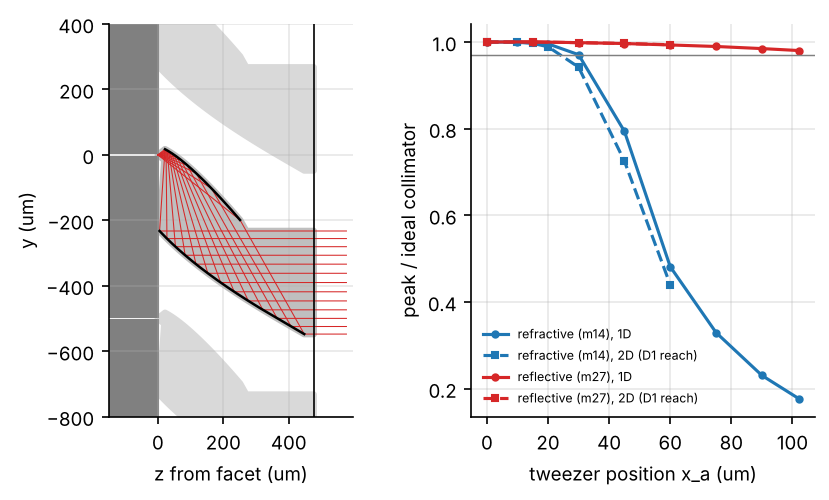
\includegraphics{../results/m27_figure.png}

\emph{Left: y-z section of the adopted block, from the facet (origin) to
the flat exit face, with rays every 6.4 deg in the glass. Grey: the
light regions, with 10 um margin, of the blocks of the neighbouring
chips at +/-0.5 mm. Dark grey: the chips (z \textless{} 0). Right: peak
of a tweezer at x\_a relative to an ideal collimator at the same s\_x,
for the refractive (m26) and reflective (m27) designs; 1D to the slit
edge, 2D within the 67 um reach of the D1 engine of the 2D model.}

\hypertarget{103-the-independent-check}{%
\subsection{10.3 The independent
check}\label{collimator-103-the-independent-check}}

We traced the adopted design through spline fits of the two mirror
curves:

\begin{itemize}
\tightlist
\item
  in 3D, with rays launched with k\_x (not with the effective index);
\item
  with the vector law of reflection;
\item
  with the optical path taken as n times the 3D length.
\end{itemize}

The phase of the k\_x = k0 s\_x component (path minus s\_x x\_exit) is
flat to below 2e-12 waves at s\_x = 0, 0.1, 0.2, 0.312 and 0.355. The
exit height equals f s n / n\_eff to 2e-10, the exit tilt is below 5e-11
rad, and the 2D effective-index lens map used by the wave model agrees
with the 3D trace to 1e-12 waves (\texttt{m27\_trace}). The refractive
design, by contrast, carries 0.30 / 1.18 / 2.86 / 3.67 waves p-v at the
same s\_x. Unit tests cover the same checks.

\hypertarget{104-performance}{%
\subsection{10.4 Performance}\label{collimator-104-performance}}

\textbf{On axis (s\_x = 0)} (\texttt{m27\_wave}):

\begin{itemize}
\tightlist
\item
  The design reproduces the ideal lens in glass and the refractive
  design to four digits: peak per guided power 1.10 relative to the
  ideal lens in air at beta = 0.7 um, y FWHM 1.35 um, crosstalk 4.0e-4 /
  8e-5 at 3 / 4 um.
\item
  With the mirror losses of real coatings, computed from the Johnson \&
  Christy constants of silver and gold (SOURCE, interpolated to 1064.4
  nm: Ag 0.04 + 7.61i, Au 0.26 + 6.97i), the mirror pair reflects:

  \begin{itemize}
  \tightlist
  \item
    99.6\% with M1 silvered and M2 used in TIR;
  \item
    98.2\% with M1 gold.
  \end{itemize}
\item
  The power per 1.2 mK tweezer is 57.7 mW (silver) or 58.5 mW (gold),
  against 57.4 mW for the refractive design with ideal AR coatings.
\item
  Real silver films reflect less than the bulk-quality constants imply
  {[}REF?{]}.
\end{itemize}

\textbf{Across the row} (\texttt{m27\_skew}, effective-index trace
verified above, downstream relay ideal):

{\footnotesize
\begin{longtable}[]{@{}>{\raggedright\arraybackslash}p{0.152\dimexpr(\linewidth-10\tabcolsep)\relax}>{\raggedright\arraybackslash}p{0.183\dimexpr(\linewidth-10\tabcolsep)\relax}>{\raggedright\arraybackslash}p{0.183\dimexpr(\linewidth-10\tabcolsep)\relax}>{\raggedright\arraybackslash}p{0.256\dimexpr(\linewidth-10\tabcolsep)\relax}>{\raggedright\arraybackslash}p{0.226\dimexpr(\linewidth-10\tabcolsep)\relax}@{}}
\toprule\noalign{}
x\_a (s\_x) & peak, reflective: 1D (2D) & peak, refractive: 1D (2D) &
crosstalk at 4 um, reflective / refractive & comb at the far row: loss,
reflective \\
\midrule\noalign{}
\endhead
\bottomrule\noalign{}
\endlastfoot
0 & 1.000 (1.000) & 1.000 (1.000) & 8.4e-5 / 8.4e-5 & 4.8e-3 \\
30 um (0.104) & 0.999 (0.999) & 0.971 (0.942) & 8.4e-5 / 3.0e-3 &
4.9e-3 \\
45 um (0.156) & 0.997 (0.997) & 0.794 (0.725) & 8.6e-5 / 8.2e-3 &
5.0e-3 \\
60 um (0.208) & 0.993 (0.994) & 0.481 (0.440) & 9.0e-5 / 6.9e-3 &
5.1e-3 \\
90 um (0.312) & 0.985 & 0.231 & 9.7e-5 / 9.0e-3 & 5.4e-3 \\
102 um (0.355, slit edge) & 0.980 & 0.177 & 1.0e-4 / 8.6e-3 & 5.5e-3 \\
\end{longtable}
}

Peaks are relative to an ideal collimator of focal length 175 um at the
same s\_x. The remaining 1.5\% at 90 um is the 2.4\% longer focal length
(a slightly wider stripe at S); relative to its own centre the
reflective tweezer keeps 0.990 at 90 um. The y centroid does not move
(below 1e-11 nm), because the mapping stays antisymmetric.

The 2D model covers \textbar x\_a\textbar{} \textless= 60 um only. Its
engine (D1, 128 ports) cannot place a tweezer beyond about 67 um for any
collimator; the 2D values m26 reported at 75 and 90 um are outside the
model (Corrected in \texttt{docs/megascale.md}, Sec. 12).

Hence one engine serves its whole segment: \textbar x\_a\textbar{}
\textless= 90 um, and in 1D to the slit edge. No common focus offset is
needed.

\textbf{Tolerances} (\texttt{m27\_tolerance}):

\begin{itemize}
\tightlist
\item
  Facet decentre and focus behave as for the refractive design: 0.973 at
  0.1 um decentre, 0.995 at 0.5 um focus and 0.977 at 1 um. The decentre
  tolerance remains a property of the facet.
\item
  Exact traces of a displaced source agree with the first-order model of
  the wave model to 1e-4 waves rms (0.2 um decentre) and 3e-4 waves rms
  (0.5 um focus).
\item
  The mirrors are about twice as sensitive to form error as the
  refractive surfaces.
\end{itemize}

{\small
\begin{longtable}[]{@{}>{\raggedright\arraybackslash}p{0.358\dimexpr(\linewidth-6\tabcolsep)\relax}>{\raggedright\arraybackslash}p{0.400\dimexpr(\linewidth-6\tabcolsep)\relax}>{\raggedright\arraybackslash}p{0.242\dimexpr(\linewidth-6\tabcolsep)\relax}@{}}
\toprule\noalign{}
form error, rms (correlation 20 um / 60 um) & reflective, adopted: mean
peak (10th percentile) & refractive (m14) \\
\midrule\noalign{}
\endhead
\bottomrule\noalign{}
\endlastfoot
5 nm & 0.996 (0.993) / 0.998 (0.996) & \\
10 nm & 0.988 (0.983) / 0.989 (0.981) & 0.995 (0.992) / 0.997 (0.994) \\
20 nm & 0.936 (0.902) / 0.957 (0.921) & 0.984 (0.970) / 0.987 (0.968) \\
50 nm & 0.70 (0.54) / 0.79 (0.67) & 0.916 (0.880) / 0.920 (0.823) \\
\end{longtable}
}

Hence the two mirrors need \textless= 10 nm rms for \textless= 2\% loss,
against about 20 nm for the refractive surfaces. The TIR variant, with
lower sensitivity, gives 0.989 / 0.956 at 10 / 20 nm (20 um
correlation).

\textbf{x axis} (\texttt{m27\_xaxis}). The folded glass path changes the
x geometry, but the effect is small.

\begin{itemize}
\tightlist
\item
  \textbf{Geometry.} The glass path of the axial ray is 749 um. The x
  slit plane lies 6.72 mm from the facet, and the virtual plane S lies
  0.29 mm behind it (the chief-ray construction of a folded system).
\item
  \textbf{Comb.} The comb therefore starts 7.51 mm from S, and the far
  row of a 32-row comb sits at 23.5 mm (23.0 mm with the refractive
  collimator). There the comb loses 4.8e-3 at x\_a = 0 and 5.5e-3 at the
  slit edge, with crosstalk at 4 um of 1.1e-4.
\item
  \textbf{Slab phase.} After its defocus is absorbed by placing the x
  lens, the glass slab adds 0.47 waves p-v of higher-order phase in s\_x
  (refractive: 0.17). Before recalibration it costs D1 tweezers at +/-60
  um less than 3e-4 in peak and 1.4 nm in position; after recalibration,
  nothing measurable.
\end{itemize}

\hypertarget{105-polarisation}{%
\subsection{10.5 Polarisation}\label{collimator-105-polarisation}}

The refractive collimator works below total internal reflection, with
real Fresnel coefficients, so it adds no s-p phase and no circular
polarisation (DERIVED). Mirrors do add one. The TE field of the chip (E
along x) is pure s-polarisation for s\_x = 0, so nothing happens on
axis. For s\_x != 0 the plane of incidence tilts, the field gains a p
component, and the s-p phase of the reflection mixes the two.

We traced the field through both mirrors in 3D (\texttt{m27\_pol}):

\begin{itemize}
\tightlist
\item
  launch: TE, the x unit vector projected transverse to each ray;
\item
  reflection: Fresnel coefficients of each coating, in a convention
  checked against a perfect conductor;
\item
  metric 1, the cross-polarised power at the centre of the tweezer: the
  coherent pupil sum, weighted by the facet far field;
\item
  metric 2, its degree of circular polarisation V.
\end{itemize}

Perfect mirrors give neither (below 1e-26). The coatings do. Their s-p
phase departs from that of a perfect mirror (the excess retardance) as
follows:

\begin{itemize}
\tightlist
\item
  silver in fused silica: 6 deg at 30 deg incidence, 31 deg at 60 deg,
  68 deg at 75 deg;
\item
  TIR: 142 to 159 deg between 45 and 75 deg, close to a half-wave.
\end{itemize}

{\small
\begin{longtable}[]{@{}>{\raggedright\arraybackslash}p{0.395\dimexpr(\linewidth-10\tabcolsep)\relax}>{\raggedright\arraybackslash}p{0.218\dimexpr(\linewidth-10\tabcolsep)\relax}>{\raggedright\arraybackslash}p{0.129\dimexpr(\linewidth-10\tabcolsep)\relax}>{\raggedright\arraybackslash}p{0.129\dimexpr(\linewidth-10\tabcolsep)\relax}>{\raggedright\arraybackslash}p{0.129\dimexpr(\linewidth-10\tabcolsep)\relax}@{}}
\toprule\noalign{}
coating (adopted layout unless stated) & x\_a = 30 um: cross-pol / V &
60 um & 90 um & 102 um \\
\midrule\noalign{}
\endhead
\bottomrule\noalign{}
\endlastfoot
perfect mirrors & 0 / 0 & 0 / 0 & 0 / 0 & 0 / 0 \\
M1 silver, M2 TIR & 1.0e-2 / -0.013 & 4.2e-2 / -0.026 & 9.6e-2 / -0.039
& 0.12 / -0.045 \\
M1 gold, M2 TIR & 1.0e-2 / -0.009 & 4.2e-2 / -0.018 & 9.5e-2 / -0.027 &
0.12 / -0.031 \\
both silver & 1.6e-3 / -0.072 & 6.7e-3 / -0.146 & 1.6e-2 / -0.223 &
2.1e-2 / -0.256 \\
TIR variant, both TIR & 3.3e-3 / +0.093 & 1.3e-2 / +0.185 & 2.9e-2 /
+0.277 & 3.8e-2 / +0.313 \\
lossless coating, excess retardance 2 deg on both & 1.5e-5 / -0.008 &
5.8e-5 / -0.015 & 1.3e-4 / -0.023 & 1.6e-4 / -0.026 \\
same, 5 deg & 9.2e-5 / -0.019 & 3.6e-4 / -0.038 & 8.0e-4 / -0.056 &
1.0e-3 / -0.064 \\
same, 10 deg & 3.7e-4 / -0.038 & 1.4e-3 / -0.075 & 3.2e-3 / -0.111 &
4.1e-3 / -0.125 \\
\end{longtable}
}

Three points follow.

(i) The circular component grows linearly with x\_a and with the excess
retardance, by about 0.011 per degree at x\_a = 90 um (two mirrors).

(ii) The layout does not help. With two silver mirrors, all 290 passing
layouts give \textbar V\textbar{} = 0.20 to 0.23 at 90 um
(\texttt{m27\_poltrade}). The least form-sensitive layouts have the
larger incidence angles, so polarisation and form tolerance do not trade
usefully.

(iii) The coating does. Using M2 in TIR, its near half-wave retardance
largely cancels the ellipticity of the silver or gold on M1. The
circular component falls to \textbar V\textbar{} \textless= 0.04
(silver) or 0.03 (gold) at 90 um, but the polarisation is then rotated
as a whole, by about 18 deg at 90 um (cross-polarised power 0.096). This
is the adopted configuration.

For alkali ground states (J = 1/2) the light shift depends on the
circular component (vector shift, proportional to V m\_F) but, apart
from a small hyperfine-induced tensor part, not on the direction of
linear polarisation. The rotation is therefore benign to first order,
and V is the figure that matters. For m\_F = 0 clock states the
first-order vector shift vanishes. We have not set a criterion for V for
the qubit encoding and bias field used in transport {[}VALUE?{]}.

If a lower V is needed, there are two options:

\begin{itemize}
\tightlist
\item
  a coating with an excess retardance of about 2 deg or less over 28 to
  77 deg on both mirrors, giving \textbar V\textbar{} \textless= 0.023
  and almost no rotation;
\item
  a compensating retarder at the x slit plane, where x encodes s\_x.
\end{itemize}

Neither is designed here. The comb teeth add a further reflection at 45
deg for half of the stacks, which we did not include.

\hypertarget{106-limits-and-next-steps}{%
\subsection{10.6 Limits and next
steps}\label{collimator-106-limits-and-next-steps}}

The trace is exact for cylindrical mirrors, and the wave model is 1D,
with 2D checks to 60 um. Coatings and TIR enter through their Fresnel
coefficients only, with no thin-film stack designed. The downstream
relay, the comb teeth (another reflection at 45 deg) and the objective
are ideal or not modelled for s\_x != 0. Polarisation is evaluated at
the pupil, before the objective.

Next steps:

\begin{itemize}
\tightlist
\item
  (i) a coating with small s-p retardance over 28 to 77 deg on M1, or a
  layout with smaller incidence angles (Sec. 10.5);
\item
  (ii) a fabrication route for a 0.48 mm fused-silica block with two
  freeform mirrors at \textless= 10 nm rms (diamond- turned moulds,
  grey-scale lithography or two-photon printing followed by reflow
  {[}REF?{]}), registered to each other to the precision the
  construction assumes;
\item
  (iii) a tolerance Monte Carlo of the block with all errors combined;
\item
  (iv) the polarisation criterion for the qubit encoding used in
  transport.
\end{itemize}

\hypertarget{verification-notes}{%
\section{Verification notes}\label{collimator-verification-notes}}

{\footnotesize
\begin{longtable}[]{@{}>{\raggedright\arraybackslash}p{0.230\dimexpr(\linewidth-8\tabcolsep)\relax}>{\raggedright\arraybackslash}p{0.129\dimexpr(\linewidth-8\tabcolsep)\relax}>{\raggedright\arraybackslash}p{0.101\dimexpr(\linewidth-8\tabcolsep)\relax}>{\raggedright\arraybackslash}p{0.539\dimexpr(\linewidth-8\tabcolsep)\relax}@{}}
\toprule\noalign{}
value & location & type & pointer \\
\midrule\noalign{}
\endhead
\bottomrule\noalign{}
\endlastfoot
designs, limits, geometry & Sec. 1, 2 & SIM & results/m14\_designs.json
(review) \\
facet R, T, capture & Sec. 1, 3 & SIM &
results/m14\_facet\_meep\_\{air,glass\}.json (review) \\
wave-model table & Sec. 1, 4 & SIM & results/m14\_wave.json (review) \\
tolerances, exact checks & Sec. 1, 5 & SIM & results/m14\_tolerance.json
(review) \\
form Monte Carlo & Sec. 5 & SIM & results/m14\_form.json (24 samples per
point; review) \\
x lens & Sec. 6 & SIM & results/m14\_xlens.json (review) \\
power plan, fibres, offsets & Sec. 1, 8 & DERIVED &
results/m14\_plan.json \\
parameter scan of the Weierstrass design & Sec. 2 & SIM &
results/m14\_scan.json \\
2D check of the adopted design (1.107) & Sec. 1 & SIM & run in session,
not stored \\
n(SiO2) 1.4496 & throughout & SOURCE & Malitson (picsim/materials.py) \\
n = 1.8, R 80 um, gap 10 um, T 250 um, AR coatings & Sec. 2, 4 & CHOICE
& design choices \\
CTE Si 2.6e-6/K, fused silica 0.55e-6/K & Sec. 7 & RECALLED & verify \\
20 MW/cm\^{}2 facet cap & Sec. 8 & CHOICE & m6 (no damage threshold
found) \\
\end{longtable}
}

\textbar{} reflective collimator: scan, construction, selection
\textbar{} Sec. 10.2 \textbar{} SIM \textbar{} results/m27\_scan.json
(review) \textbar{} \textbar{} 3D trace: W, mapping, effective-index
check \textbar{} Sec. 10.3 \textbar{} SIM \textbar{}
results/m27\_trace.json \textbar{} \textbar{} wave model, mirror
reflectance, power \textbar{} Sec. 10.4 \textbar{} SIM \textbar{}
results/m27\_wave.json (review) \textbar{} \textbar{} skew, comb at the
far row \textbar{} Sec. 10.4 \textbar{} SIM \textbar{}
results/m27\_skew.json, results/m27\_skew\_summary.json (review)
\textbar{} \textbar{} tolerances, form Monte Carlo \textbar{} Sec. 10.4
\textbar{} SIM \textbar{} results/m27\_tolerance.json (24 samples per
point; review) \textbar{} \textbar{} x geometry, slab phase \textbar{}
Sec. 10.4 \textbar{} SIM \textbar{} results/m27\_xaxis.json (review)
\textbar{} \textbar{} polarisation, coating trade \textbar{} Sec. 10.5
\textbar{} SIM \textbar{} results/m27\_pol.json,
results/m27\_poltrade.json (review) \textbar{} \textbar{} n(Ag), n(Au)
at 1064.4 nm \textbar{} Sec. 10.4, 10.5 \textbar{} SOURCE \textbar{}
Johnson \& Christy, Phys. Rev. B 6, 4370 (1972),
doi:10.1103/PhysRevB.6.4370; refractiveindex.info tables retrieved
2026-11-09, interpolated \textbar{} \textbar{} 0.5 mm length limit, 10
um clearance, 20 um radius limit \textbar{} Sec. 10.2 \textbar{} CHOICE
\textbar{} design choices \textbar{}

Open placeholders: {[}REF?{]} UV-adhesive shrinkage and creep at the 0.1
um level; {[}REF?{]} placement accuracy of two-photon-printed
micro-optics on chip facets; {[}VALUE?{]} CW power handling of
acousto-optic shifters at 3 W, 1064 nm; {[}VALUE?{]} available
single-frequency 1064 nm power at 40 to 55 W; {[}REF?{]} reflectance of
deposited silver on fused silica at 1064 nm; {[}REF?{]} fabrication of
freeform glass micro-mirrors at \textless= 10 nm rms; {[}VALUE?{]}
tolerable circular polarisation of the transport tweezers.

\hypertarget{independent-rows-without-acousto-optic-frequency-offsets}{%
\chapter{Independent rows without acousto-optic frequency
offsets}\label{row_coherence-independent-rows-without-acousto-optic-frequency-offsets}}

Follow-up to \texttt{docs/stacked\_relay.md} (Sec. 5) and
\texttt{docs/collimator.md} (Sec. 8), which proposed one acousto-optic
frequency shifter per chip. Code: \texttt{scripts/m15\_coherence.py}
(vector focusing in \texttt{picsim/opa/stack.py},
\texttt{Focus2D.field\_vector}); results \texttt{results/m15\_*.json}.
Values are SIM or DERIVED, valid in the regime stated, and should be
reviewed before they are quoted.

\hypertarget{1-result}{%
\section{Result}\label{row_coherence-1-result}}

Per-chip frequency offsets are not needed. The same decoupling is
obtained with one electro-optic phase modulator on the seed laser,
driven with Gaussian noise of about 3 rad rms and 1 to 2 GHz bandwidth,
ahead of the 1:16 split. Each chip\textquotesingle s feed is then given
a different fibre length, in steps of at least three correlation lengths
(about 0.3 m at 2 GHz, at most 5 m in total). Within one chip all paths
agree to better than a millimetre, so the light stays coherent and route
E is unaffected. Between chips the relative phase becomes a random
process with correlation time below 1 ns, so the atoms see the time
average.

A fully passive alternative, orthogonal linear polarisation on alternate
chips, meets the dynamic criteria. It leaves a slow depth wander of
0.4\% rms and needs a polarisation-insensitive objective.

Perturbation of a tweezer by all other rows within +/-16 um (both sides;
rms over drifting relative phases, pairs in quadrature; 4 um rows, full
rows of 41 tweezers):

{\footnotesize
\begin{longtable}[]{@{}>{\raggedright\arraybackslash}p{0.192\dimexpr(\linewidth-10\tabcolsep)\relax}>{\raggedright\arraybackslash}p{0.256\dimexpr(\linewidth-10\tabcolsep)\relax}>{\raggedright\arraybackslash}p{0.081\dimexpr(\linewidth-10\tabcolsep)\relax}>{\raggedright\arraybackslash}p{0.169\dimexpr(\linewidth-10\tabcolsep)\relax}>{\raggedright\arraybackslash}p{0.302\dimexpr(\linewidth-10\tabcolsep)\relax}@{}}
\toprule\noalign{}
option & added hardware & power & static depth / position (rms) & when a
tweezer moves 0.25 um: depth / position (rms) \\
\midrule\noalign{}
\endhead
\bottomrule\noalign{}
\endlastfoot
all chips coherent, no measure & none & 1 & 2.3\% / 9.2 nm & 2.3e-3 /
5.1 nm \\
per-chip AOM offsets & 16 AOMs at 2.6 to 3.4 W & 1 (+ AOM loss) & 1.8e-4
/ 0.09 nm & 2e-5 / 0.05 nm \\
\textbf{common phase noise + fibre delays} & \textbf{1 EOM on the seed,
noise source, \textless= 5 m fibre} & \textbf{1} & \textbf{1.6e-4 / 0.07
nm} & \textbf{2e-5 / 0.04 nm} \\
alternating x / y polarisation & half-wave-plate strips (passive) & 1 &
4.2e-3 / 2.5 nm & 1.1e-3 / 1.6 nm \\
y apodiser a = 0.65 & graded mirror (passive) & 1.84 & 5.2e-3 / 4.1 nm &
1.0e-3 / 1.8 nm \\
polarisation + apodiser a = 0.8 & passive & 1.55 & 2.8e-3 / 1.8 nm &
5.7e-4 / 0.7 nm \\
\end{longtable}
}

(Criteria used for the rows within a chip: others\textquotesingle{}
depth change \textless{} 3e-3 and position change \textless{} 5 nm when
a tweezer moves; proposal budget 10 nm rms position noise.) Leaving all
chips coherent breaks the position budget: 9.2 nm rms of slow wander
plus 5.1 nm when neighbours move.

\hypertarget{2-what-the-frequency-offset-actually-does}{%
\section{What the frequency offset actually
does}\label{row_coherence-2-what-the-frequency-offset-actually-does}}

Light from chip m reaches row m+1 at about 1e-4 of the peak intensity
(module 13). If the two chips are mutually coherent, this field
interferes with the neighbour\textquotesingle s own field, and the depth
changes by about 2 sqrt(epsilon) cos(phi), where phi is the relative
optical phase of the two feeds. Separate fibres let phi drift with
temperature and acoustics. A frequency offset delta f makes phi advance
at 2 pi delta f. When delta f is far above the trap frequencies, the
atom sees only the time average, and the interference term vanishes. Any
process that randomises phi on time scales much shorter than the trap
period does the same. A frequency offset is one such process; a common
random phase seen with different delays is another.

\hypertarget{3-common-phase-modulation-with-fibre-delays}{%
\section{Common phase modulation with fibre
delays}\label{row_coherence-3-common-phase-modulation-with-fibre-delays}}

If the seed carries a phase phi(t) and chip m receives it after a delay
tau\_m, the relative phase of chips m and n is phi(t - tau\_m) - phi(t -
tau\_n). Its mean contribution to the interference is the field
coherence \textbar\textless exp(i {[}phi(t) - phi(t -
tau){]})\textgreater\textbar{} at tau = tau\_m - tau\_n.

{\footnotesize
\begin{longtable}[]{@{}>{\raggedright\arraybackslash}p{0.186\dimexpr(\linewidth-8\tabcolsep)\relax}>{\raggedright\arraybackslash}p{0.291\dimexpr(\linewidth-8\tabcolsep)\relax}>{\raggedright\arraybackslash}p{0.314\dimexpr(\linewidth-8\tabcolsep)\relax}>{\raggedright\arraybackslash}p{0.209\dimexpr(\linewidth-8\tabcolsep)\relax}@{}}
\toprule\noalign{}
modulation & residual coherence, delays 2 to 15 bits & with finite
modulator bandwidth (10-90\% rise 0.3 bit) & at arbitrary (non-integer)
delays \\
\midrule\noalign{}
\endhead
\bottomrule\noalign{}
\endlastfoot
binary 0/pi m-sequence, N = 1023 & 9.8e-4 (= 1/N) & 4.1e-2 (carrier
0.12) & as integer \\
same, depth error +5\% / +10\% & 5.2e-3 / 2.4e-2 & & \\
Zadoff-Chu polyphase, N = 1021 & \textless{} 1e-13 & 4.7e-3 & 6.2e-2 \\
\textbf{Gaussian phase noise, 3 rad rms} & 4.2e-3 (record-limited;
ensemble exp(-9) = 1.2e-4) & inherent & 7.2e-3 \\
Gaussian phase noise, 4 rad rms & 5.6e-3 (record-limited) & inherent &
8.2e-3 \\
\end{longtable}
}

Binary modulation is fragile. Every 0-to-pi and pi-to-0 transition
passes through +pi/2, so a band-limited modulator leaves a carrier (0.12
at 0.3-bit rise), and the delays must be exact multiples of the bit
length. Polyphase codes have perfect autocorrelation but also need exact
delays. Gaussian phase noise of 3 rad rms needs neither: the carrier is
exp(-sigma\^{}2/2), and any delay longer than about three correlation
times decorrelates. The 4e-3 to 8e-3 above is the statistical floor of a
32,768-bit record. What the atom sees is set by the low-frequency
density of the interference term, 0.40/B. For the coherent term of
module 13 (2 sqrt(epsilon) = 2.1e-2), this gives S\_I(2 nu\_trap) =
8.8e-14/Hz at B = 2 GHz. The parametric heating rate Gamma = pi\^{}2
nu\^{}2 S\_I(2 nu) (O\textquotesingle Hara et al.,
arXiv:physics/0003049, used in module 3) is then 6e-3 s\^{}-1 at nu = 84
kHz, an energy e-folding time above 2 minutes. At B = 0.5 GHz it is
2.4e-2 s\^{}-1.

\textbf{Spectral width.} With 3 rad of noise at correlation rate B, the
optical spectrum is Gaussian with rms width 0.67 B (1.35 GHz, 5 pm, at B
= 2 GHz). Its effect on the tweezers comes through the diffractive
objective\textquotesingle s axial chromatic shift (16 um/nm, DERIVED for
f = 17.3 mm with f proportional to 1/lambda) and the lateral scaling x
proportional to lambda:

{\small
\begin{longtable}[]{@{}>{\raggedright\arraybackslash}p{0.092\dimexpr(\linewidth-10\tabcolsep)\relax}>{\raggedright\arraybackslash}p{0.218\dimexpr(\linewidth-10\tabcolsep)\relax}>{\raggedright\arraybackslash}p{0.172\dimexpr(\linewidth-10\tabcolsep)\relax}>{\raggedright\arraybackslash}p{0.218\dimexpr(\linewidth-10\tabcolsep)\relax}>{\raggedright\arraybackslash}p{0.299\dimexpr(\linewidth-10\tabcolsep)\relax}@{}}
\toprule\noalign{}
B & optical rms width & axial rms smear & peak & lateral rms smear at 60
um \\
\midrule\noalign{}
\endhead
\bottomrule\noalign{}
\endlastfoot
0.5 GHz & 0.34 GHz & 0.02 um & 0.99997 & 0.07 nm \\
2 GHz & 1.35 GHz & 0.08 um & 0.9998 & 0.29 nm \\
10 GHz & 6.7 GHz & 0.41 um & 0.995 & 1.4 nm \\
\end{longtable}
}

The spectrum is symmetric about the carrier, so the mean light shift at
the double-magic wavelength is unchanged to first order. The
second-order term needs the curvature of the differential polarisability
{[}VALUE?{]}.

\textbf{Coherence inside a chip.} Path differences within a chip and its
relay are at most about 1 mm (about 5 ps). With a 0.5 ns correlation
time (B = 2 GHz) and sigma = 3 rad, the coherence loss is sigma\^{}2
(tau/tau\_c)\^{}2 / 2 \textasciitilde{} 5e-4. The least-squares
synthesis of route E therefore sees an essentially coherent source.

\textbf{Hardware.} A fibre-coupled LiNbO3 phase modulator on the
low-power seed and a Gaussian noise source amplified to about 1 V\_pi
rms (3 rad) over 1 to 2 GHz. Extra fibre is 0, 0.3, 0.6 ... 4.5 m on the
16 chip feeds, before or after the amplifiers. A seed broadened to about
1 GHz also raises the stimulated-Brillouin threshold of the high-power
amplifier and delivery fibres, which carry 3 W each {[}REF?, RECALLED:
SBS suppression by phase modulation is standard in high-power
single-frequency fibre amplifiers{]}. If the chosen amplifier already
broadens its seed for this reason, the only addition is the fibre
delays. Compared with 16 AOMs, this removes 16 RF drivers and the AOM
insertion loss (about 15\% each {[}VALUE?{]}).

\hypertarget{4-passive-options}{%
\section{Passive options}\label{row_coherence-4-passive-options}}

\textbf{Orthogonal polarisation on alternate chips.} A half-wave-plate
strip in front of every other chip, in the collimated region after the
collimators, rotates its light to y. We computed vector focal fields
(Richards-Wolf, aplanatic NA 0.5 objective) and summed the intensity
over Ex, Ey and Ez (scalar light shift):

{\small
\begin{longtable}[]{@{}>{\raggedright\arraybackslash}p{0.222\dimexpr(\linewidth-8\tabcolsep)\relax}>{\raggedright\arraybackslash}p{0.286\dimexpr(\linewidth-8\tabcolsep)\relax}>{\raggedright\arraybackslash}p{0.302\dimexpr(\linewidth-8\tabcolsep)\relax}>{\raggedright\arraybackslash}p{0.190\dimexpr(\linewidth-8\tabcolsep)\relax}@{}}
\toprule\noalign{}
separation & polarisations & static: depth / position (worst phase) &
moving: depth / position \\
\midrule\noalign{}
\endhead
\bottomrule\noalign{}
\endlastfoot
4 um & orthogonal & 8.4e-4 / 1.2 nm & 1.6e-4 / 0.3 nm \\
8 um & parallel & 3.3e-3 / 2.1 nm & 1.1e-3 / 1.4 nm \\
12 um & orthogonal & 5.0e-5 / 0.3 nm & 4.4e-5 / 0.1 nm \\
16 um & parallel & 2.4e-3 / 0.4 nm & 3.5e-4 / 0.6 nm \\
\end{longtable}
}

At NA 0.5 the orthogonal neighbours\textquotesingle{} interference falls
by a factor of 26 (the residual comes from the depolarisation of
high-angle rays, mainly via Ez). The rows two apart (8 um) share a
polarisation and then dominate. The moving-tweezer criteria are met, and
the position budget too (2.5 nm rms). The static depth wanders by 0.4\%
rms with the fibre phases, at Hz to kHz rates, far below twice the trap
frequencies.

Three costs follow. (i) The meta-objective must be
polarisation-insensitive (propagation-phase meta-atoms with fourfold
symmetry rather than geometric phase). (ii) Where the orthogonal fields
overlap, the polarisation becomes elliptical in proportion to their
relative phase, which produces a vector light shift. Our estimate, from
the far-detuned alkali formula for Cs at 1064 nm, is a vector-to-scalar
ratio of about 0.09 g\_F m\_F per unit ellipticity (RECALLED, verify).
With an ellipticity of up to about 2e-2 at 4 um, this is about 2e-3 g\_F
m\_F of the trap depth: up to tens of kHz for stretched states, zero to
first order for clock states (m\_F = 0). (iii) Only two orthogonal
states exist, so rows two apart stay coherent.

\textbf{Passive y apodiser.} A Gaussian graded-transmission (or
graded-reflectivity) filter at the plane of the y telescope conjugate to
the pupil apodises all chips at once. It lowers the 1D crosstalk at 4 um
from 8.4e-5 to 3.5e-6 (a = 0.65 pupil radii, beta = 0.7 um). However, it
costs a factor 1.84 in power and widens the y spot from 1.35 to 1.73 um.
In 2D, the coherent sum of a full row, with the circular pupil, still
leaves 4.7e-3 of static depth change at 4 um. It is not competitive.

\hypertarget{5-recommendation}{%
\section{Recommendation}\label{row_coherence-5-recommendation}}

Use common phase modulation with fibre delays in place of per-chip AOMs:
one modulator, no power penalty, and the same row independence as
frequency offsets. Alternating polarisation costs nothing to add, and it
gives a second, independent factor of about 26 on the nearest rows if
the modulation fails or is switched off.

Next step (i) is simulated in \texttt{docs/pm\_am.md} (filters narrower
than about 100 pm and reflection pairs with R1 R2 \textgreater{} 1.7e-3
must be avoided; a representative chain gives -134.5 dB/Hz). Next steps:
(i) measure the delayed self-coherence of the modulated seed after the
amplifier (PM-to-AM conversion by any spectral filtering adds intensity
noise at GHz; its density at 2 nu\_trap should be checked); (ii) choose
the noise drive (or a deterministic multi-tone drive with the same
autocorrelation); (iii) obtain the second-order differential light shift
of the 1064.4350 nm double-magic condition over +/-5 pm.

\hypertarget{verification-notes}{%
\section{Verification notes}\label{row_coherence-verification-notes}}

{\footnotesize
\begin{longtable}[]{@{}>{\raggedright\arraybackslash}p{0.262\dimexpr(\linewidth-8\tabcolsep)\relax}>{\raggedright\arraybackslash}p{0.131\dimexpr(\linewidth-8\tabcolsep)\relax}>{\raggedright\arraybackslash}p{0.179\dimexpr(\linewidth-8\tabcolsep)\relax}>{\raggedright\arraybackslash}p{0.429\dimexpr(\linewidth-8\tabcolsep)\relax}@{}}
\toprule\noalign{}
value & location & type & pointer \\
\midrule\noalign{}
\endhead
\bottomrule\noalign{}
\endlastfoot
option table & Sec. 1 & SIM/DERIVED & results/m15\_summary.json from
m15\_coherent and m15\_prbs (review) \\
2D coherent / incoherent, vector fields & Sec. 1, 4 & SIM &
results/m15\_coherent.json (review) \\
residual coherence, spectra, chromatic smear & Sec. 3 & SIM &
results/m15\_prbs.json (review) \\
apodiser scan & Sec. 4 & SIM & results/m15\_apod.json (review) \\
heating rates & Sec. 3 & DERIVED & O\textquotesingle Hara et al.,
arXiv:physics/0003049 (used and checked in module 3), density from
m15\_prbs \\
16 um/nm axial chromatic shift & Sec. 3 & DERIVED & f/lambda for a
diffractive objective, f = 17.3 mm \\
vector-to-scalar ratio 0.09 g\_F m\_F & Sec. 4 & RECALLED & far-detuned
formula (Grimm et al., arXiv:physics/9902072), not read this session;
counter-rotating terms neglected \\
3 rad rms, B 1-2 GHz, 0.3 m delay steps & Sec. 1, 3 & CHOICE & design
choices \\
\end{longtable}
}

Open placeholders: {[}REF?{]} SBS suppression by phase modulation in
high-power 1064 nm fibre amplifiers; {[}VALUE?{]} AOM insertion loss at
3 W; {[}VALUE?{]} second-order differential light shift of the
double-magic condition over a 5 pm spectrum; vector polarisability of Cs
at 1064 nm from a primary source.

\hypertarget{phase-to-intensity-conversion-of-the-decorrelating-phase-noise}{%
\chapter{Phase-to-intensity conversion of the decorrelating phase
noise}\label{pm_am-phase-to-intensity-conversion-of-the-decorrelating-phase-noise}}

Follow-up to \texttt{docs/row\_coherence.md}, which replaces per-chip
frequency shifters by common Gaussian phase noise (3 rad rms,
correlation rate B = 2 GHz) on the seed. Code:
\texttt{scripts/m16\_pm\_am.py}; results
\texttt{results/m16\_pm\_am.json} (+ .png). Values are SIM, valid for
the element models and parameter ranges stated (CHOICE ranges, not
measured components), and should be reviewed before they are quoted.

\hypertarget{1-result}{%
\section{Result}\label{pm_am-1-result}}

Phase noise alone leaves the intensity constant: the simulated control
gives -376 dB/Hz, the numerical floor. Intensity noise appears only
where an element filters the spectrum. Two elements matter: narrow
band-pass filters and multipath (any delayed copy, from two
reflections). Gain tilt, fibre dispersion and polarisation crosstalk in
PM fibre are harmless. The criterion is a parametric heating rate Gamma
= pi\^{}2 nu\^{}2 S(2 nu) of at most 0.1 s\^{}-1 at nu = 84 kHz, i.e. a
relative intensity noise (RIN) density at 168 kHz of S \textless=
1.4e-12/Hz (-118 dB/Hz). A representative chain gives -134.5 dB/Hz
(Gamma = 2.5e-3 s\^{}-1), 16 dB inside the criterion. The design rules
that follow are: (i) no filter narrower than about 100 pm (20 times the
1.35 GHz rms modulation width) in the light path; (ii) the product of
any two reflections in the chain, R1 R2, below 1.7e-3 (amplitude r
\textless= 0.042), i.e. no pair of uncoated glass surfaces in series.

\hypertarget{2-elements}{%
\section{Elements}\label{pm_am-2-elements}}

RIN density in the 100-300 kHz band, record 131 us at 16 GS/s, worse of
two relative phases for copies:

{\footnotesize
\begin{longtable}[]{@{}>{\raggedright\arraybackslash}p{0.293\dimexpr(\linewidth-10\tabcolsep)\relax}>{\raggedright\arraybackslash}p{0.223\dimexpr(\linewidth-10\tabcolsep)\relax}>{\raggedright\arraybackslash}p{0.210\dimexpr(\linewidth-10\tabcolsep)\relax}>{\raggedright\arraybackslash}p{0.153\dimexpr(\linewidth-10\tabcolsep)\relax}>{\raggedright\arraybackslash}p{0.121\dimexpr(\linewidth-10\tabcolsep)\relax}@{}}
\toprule\noalign{}
element & case & RIN rms (all frequencies) & RIN at 168 kHz & heating
rate \\
\midrule\noalign{}
\endhead
\bottomrule\noalign{}
\endlastfoot
amplifier gain tilt & 0.05 / 0.5 / 5 dB/nm & 6e-5 / 6e-4 / 6e-3 & -237 /
-216 / -182 dB/Hz & \textless{} 1e-6 s\^{}-1 \\
band-pass, FWHM 1 nm, offset 250 pm & ASE filter & 7e-3 & -173 dB/Hz &
\textless{} 1e-6 s\^{}-1 \\
band-pass, FWHM 100 pm, centred / offset 25 pm & & 1.0e-2 / 7.0e-2 &
-130 / -133 dB/Hz & 7e-3 / 3e-3 s\^{}-1 \\
band-pass, FWHM 30 pm, centred / offset 7.5 pm & & 9.6e-2 / 0.21 &
\textbf{-110 / -113 dB/Hz} & \textbf{0.70 / 0.37 s\^{}-1} \\
multipath, R1 = R2 = 1e-2, delay \textgreater= 0.3 ns & two -20 dB
reflections & 1.4e-2 & -130 dB/Hz & 7e-3 s\^{}-1 \\
multipath, R1 = R2 = 1e-2, delay 0.1 / 0.01 ns & on chip, mm scale &
7e-3 / 1e-4 & -133 / -171 dB/Hz & 3e-3 / 1e-6 s\^{}-1 \\
multipath, R1 = R2 = 1e-3 or 1e-4, any delay & & \textless= 1.4e-3 &
\textless= -149 dB/Hz & \textless= 8e-5 s\^{}-1 \\
PM fibre, PER -20 dB, 5 / 20 m (DGD 1.2 ps/m) & then the chip TE guide
as polariser & 3e-4 / 5e-3 & -161 / -137 dB/Hz & 6e-6 / 1.4e-3
s\^{}-1 \\
dispersion, 20 ps\^{}2/km, 5 m to 1 km & & \textless= 8e-4 & \textless{}
-280 dB/Hz & 0 \\
chain (Sec. 3) & & 6.9e-3 & -134.5 dB/Hz & 2.5e-3 s\^{}-1 \\
\end{longtable}
}

The structure follows from the physics. Gain tilt and dispersion respond
to the instantaneous frequency, the time derivative of the phase, whose
spectrum vanishes towards low frequency. So their intensity noise lies
at GHz, not at 168 kHz. A delayed copy of amplitude r produces an
intensity term 2 r cos(phi(t) - phi(t - tau)). Once tau exceeds the
correlation time (about 0.3 ns), this term is a random telegraph-like
signal of variance 2 r\^{}2 spread over about B, so S \textasciitilde{}
4 r\^{}2 x 0.40 / B (the 0.40/B is the low-frequency density found in
module 15). For tau far below the correlation time the term is quadratic
in the phase increment and much smaller. A band-pass narrower than the
spectrum is the multipath effect again: it is a delay distributed over
its impulse response, about 1/(pi x FWHM) = 40 ps for 30 pm.

\textbf{Dependence on B} (r = 1e-2): at tau = 1 ns, S is -125, -130 and
-138 dB/Hz for B = 0.5, 2 and 8 GHz, because the noise spreads as 1/B.
At tau = 0.1 ns, B = 0.5 GHz is the quietest (-170 dB/Hz): there the
copy is still inside the correlation time. A higher B therefore helps
against long-delay reflections and hurts against short ones. B = 2 GHz
is a reasonable middle.

\hypertarget{3-representative-chain}{%
\section{Representative chain}\label{pm_am-3-representative-chain}}

Amplifier tilt 0.5 dB/nm; ASE filter of 1 nm FWHM, offset 250 pm; PM
fibre 5 m with -20 dB polarisation crosstalk; two -30 dB connector
reflections 5 m apart (tau = 25 ns); an on-chip etalon between a -30 dB
input facet and the 2.3\% glued emitter facet (module 14), 190 ps round
trip; 5 m of dispersion. Result: RIN rms 6.9e-3 (at GHz), -134.5 dB/Hz
at 168 kHz, Gamma = 2.5e-3 s\^{}-1 (energy e-folding about 7 min). The
on-chip etalon and the connector pair dominate.

\hypertarget{4-comparison-with-no-modulation}{%
\section{Comparison with no
modulation}\label{pm_am-4-comparison-with-no-modulation}}

Without phase modulation, the same reflections do not produce noise at
168 kHz. Instead they give a slow intensity offset 2 r cos(Phi) that
follows the drift of the path phase Phi: 2\% for r = 1e-2, at Hz to kHz
rates. The modulation converts this slow, uncontrolled offset into
broadband noise of the same rms. Spread over GHz, it deposits only 1e-13
to 1e-12 /Hz near the trap frequencies. Phase noise therefore helps
against parasitic etalons as well as against row crosstalk, provided
rule (ii) holds.

\hypertarget{5-limits-and-what-to-measure}{%
\section{Limits and what to
measure}\label{pm_am-5-limits-and-what-to-measure}}

The elements are linear and treated separately. Gain dynamics of the
amplifier (which can suppress or shape slow intensity noise) and
nonlinear effects (self-phase modulation, stimulated Brillouin
scattering) are not modelled. The criterion uses the radial frequency;
the axial frequency is lower and its parametric resonance lies where the
RIN density is the same, so the conclusion holds. Measurement: delayed
self-heterodyne or direct RIN of the modulated, amplified light after
the full chain, with the modulation on and off, at 10 kHz to 1 MHz. The
prediction to test is a floor below -130 dB/Hz with a 1 nm ASE filter
and AR-coated components.

\hypertarget{verification-notes}{%
\section{Verification notes}\label{pm_am-verification-notes}}

{\footnotesize
\begin{longtable}[]{@{}>{\raggedright\arraybackslash}p{0.265\dimexpr(\linewidth-8\tabcolsep)\relax}>{\raggedright\arraybackslash}p{0.146\dimexpr(\linewidth-8\tabcolsep)\relax}>{\raggedright\arraybackslash}p{0.146\dimexpr(\linewidth-8\tabcolsep)\relax}>{\raggedright\arraybackslash}p{0.444\dimexpr(\linewidth-8\tabcolsep)\relax}@{}}
\toprule\noalign{}
value & location & type & pointer \\
\midrule\noalign{}
\endhead
\bottomrule\noalign{}
\endlastfoot
all RIN densities, heating rates & Sec. 1-4 & SIM &
results/m16\_pm\_am.json (review) \\
element parameter ranges & Sec. 2, 3 & CHOICE & stated ranges, not
component data \\
PM-fibre DGD 1.2 ps/m, beta2 20 ps\^{}2/km & Sec. 2 & RECALLED & verify
for the chosen fibre \\
Gamma = pi\^{}2 nu\^{}2 S(2 nu) & Sec. 1 & SOURCE &
O\textquotesingle Hara et al., arXiv:physics/0003049 (module 3) \\
0.1 s\^{}-1 criterion & Sec. 1 & CHOICE & energy doubling time
\textasciitilde7 s \\
\end{longtable}
}

\hypertarget{3d-transport-with-handoff-between-the-static-array-and-the-moving-tweezers}{%
\chapter{3D transport with handoff between the static array and the
moving
tweezers}\label{transport3d-3d-transport-with-handoff-between-the-static-array-and-the-moving-tweezers}}

\begin{quote}
Follow-up (\texttt{docs/rearrangement.md}): slower handoff steps (200 us
ramps, 400 us lane steps) cut the heating per handoff to 0.12 uK at 0.1
/ 0.3 mK (1D quantum, handoff and lane axis); with the x move it is
about 0.3 uK per move (quantum, 0.12 + 0.17 uK), and the 3D classical
run gives 0.16 uK. The shallow 0.3 mK point is then also the low-heating
point. The static array\textquotesingle s depth uniformity is not a
constraint.
\end{quote}

Follow-up to \texttt{docs/scaling\_beyond.md}, whose 1D model left out
handoff, the static array and the third dimension. Code:
\texttt{picsim/transport3d.py}, \texttt{scripts/m18\_transport3d.py};
results \texttt{results/m18\_*.json}, \texttt{results/m18\_trap.npz};
tests \texttt{tests/test\_transport3d.py}. Values are SIM (classical
Monte Carlo) and valid in the regime stated. They should be reviewed
before they are quoted.

\hypertarget{1-result}{%
\section{Result}\label{transport3d-1-result}}

A moving tweezer of the adopted design picks an atom out of a static
1075 nm trap, carries it 12 or 40 um and drops it into an empty static
trap. With the right depths and path, it delivers 3,000 of 3,000
simulated atoms (loss \textless{} 1e-3 at 95\% confidence) and heats
them by 1 to 2 uK per move. Three conditions are needed:

(i) \textbf{Move along lanes between the rows, not along the rows.} A
tweezer that crosses empty static sites on its row loses 45 to 95\% of
atoms at most settings. Only a moving trap five times deeper than the
static traps, moving slowly (400 us), recovers 99.1 to 99.7\%. Along a
lane 2 um off the row, reached with the row-select y tilt, the static
traps are 1.6e-5 of their depth away and transport is clean. All
tweezers of a stack enter and leave the lanes together.

(ii) \textbf{Moving depth at least three times the static hold depth.}
At a ratio of 1.5, 5\% of atoms stay behind; at 2, 3 to 5\% are lost; at
3, 99.5 to 99.9\% are delivered with about 10 uK of heating per move; at
5, 99.6 to 100\% with 1 to 2.6 uK.

(iii) \textbf{Hold depth of about 20 kT.} Atoms waiting next to a lane
feel the passing tweezer\textquotesingle s out-of-focus light (6 to 15\%
of its peak at 1.5 to 2.5 um, a few um from focus). At a hold depth of
10 kT, 1 to 2\% of them are lost from the hot tail; at 20 kT, none of
3,000.

Operating points (12 um move in 400 us, 100 us ramps, 200 kHz updates,
lane 2 um):

{\footnotesize
\begin{longtable}[]{@{}>{\raggedright\arraybackslash}p{0.097\dimexpr(\linewidth-16\tabcolsep)\relax}>{\raggedright\arraybackslash}p{0.076\dimexpr(\linewidth-16\tabcolsep)\relax}>{\raggedright\arraybackslash}p{0.110\dimexpr(\linewidth-16\tabcolsep)\relax}>{\raggedright\arraybackslash}p{0.172\dimexpr(\linewidth-16\tabcolsep)\relax}>{\raggedright\arraybackslash}p{0.131\dimexpr(\linewidth-16\tabcolsep)\relax}>{\raggedright\arraybackslash}p{0.131\dimexpr(\linewidth-16\tabcolsep)\relax}>{\raggedright\arraybackslash}p{0.131\dimexpr(\linewidth-16\tabcolsep)\relax}>{\raggedright\arraybackslash}p{0.152\dimexpr(\linewidth-16\tabcolsep)\relax}@{}}
\toprule\noalign{}
atoms & hold & moving & delivered & heating per move & waiting atoms
lost & power per tweezer & 720 tweezers \\
\midrule\noalign{}
\endhead
\bottomrule\noalign{}
\endlastfoot
5 uK & 0.1 mK & 0.3 mK & 3000/3000 & 9.9 uK & 0/3000 & 14 mW & 10 W \\
5 uK & 0.1 mK & 0.5 mK & 3000/3000 & 1.8 uK & \textless= 2/3000 & 24 mW
& 17 W \\
10 uK & 0.2 mK & 0.6 mK & 3000/3000 & 10.0 uK & 0/3000 & 29 mW & 21 W \\
10 uK & 0.2 mK & 1.0 mK & 3000/3000 & 0.9 uK & \textless= 3/3000 & 48 mW
& 34 W \\
\end{longtable}
}

(Power scales from 57 mW at 1.2 mK, \texttt{docs/collimator.md}.) Hence
the required depth is set by the atom temperature, not by the move:
about 60 kT for the moving trap, or 100 kT for low heating. Cooling the
atoms to 5 uK halves the laser power. The 1D estimate of 0.2 mK in
\texttt{docs/scaling\_beyond.md} is too optimistic once handoff and
waiting atoms are included.

\hypertarget{2-model}{%
\section{Model}\label{transport3d-2-model}}

\textbf{Moving tweezer.} The intensity of one tweezer of design D1 (BPM
response, least-squares synthesis), through the Weierstrass + aplanat
collimator and the circular NA 0.5 pupil, computed by scalar focusing
with defocus on a grid of 7 x 6 x 20 um (\texttt{m18\_field}). FWHM 1.73
um (x, along the row), 1.37 um (y), 9.8 um (z); trap frequencies at 1 mK
54, 67 and 22 kHz. Its shape is held fixed while it moves; positions and
depth are sampled and held at 200 kHz.

\textbf{Static array.} Gaussian beams at 1075 nm, waist 0.85 um
(CHOICE), Rayleigh range 2.1 um, 4 um pitch, three rows of 15 sites, all
at one global hold depth (a fixed meta-optic array cannot switch single
sites). The two wavelengths add incoherently.

\textbf{Atoms.} Cs, classical, velocity Verlet with 0.25 us steps,
gravity along y, 1,500 to 3,000 atoms per case. Each starts in a thermal
distribution (harmonic sampling), truncated to atoms bound in the real
Gaussian site.

\textbf{Sequence.} Ramp the moving trap up on the source site (sin\^{}2,
100 us); move 2 um in y to the lane (100 us); move in x (minimum jerk);
move back to the row (100 us); ramp down on the target (100 us); hold
100 us. An atom counts as delivered if it is bound in the target static
trap after the moving trap is off.

\hypertarget{3-tolerances}{%
\section{Tolerances}\label{transport3d-3-tolerances}}

Hold 0.1 mK, moving 0.3 / 0.5 mK, 10 uK, lane, 12 um in 400 us (fraction
delivered):

{\small
\begin{longtable}[]{@{}>{\raggedright\arraybackslash}p{0.331\dimexpr(\linewidth-8\tabcolsep)\relax}>{\raggedright\arraybackslash}p{0.202\dimexpr(\linewidth-8\tabcolsep)\relax}>{\raggedright\arraybackslash}p{0.234\dimexpr(\linewidth-8\tabcolsep)\relax}>{\raggedright\arraybackslash}p{0.234\dimexpr(\linewidth-8\tabcolsep)\relax}@{}}
\toprule\noalign{}
parameter & value & moving 0.3 mK & moving 0.5 mK \\
\midrule\noalign{}
\endhead
\bottomrule\noalign{}
\endlastfoot
none & & 0.9993 & 0.9993 \\
axial offset of the 1064 and 1075 nm foci & 0.5 / 1 / 2 / 4 um & 0.998 /
0.995 / 0.939 / 0.455 & 0.995 / 0.997 / 0.957 / 0.902 \\
lateral offset, y & 0.1 / 0.2 / 0.4 um & 1.000 / 0.998 / 0.999 & 1.000 /
1.000 / 0.998 \\
lateral offset, x & 0.1 / 0.2 / 0.4 um & 0.998 / 1.000 / 0.998 & 1.000 /
1.000 / 0.999 \\
ramp time & 25 / 200 us & 0.994 / 0.998 & 0.993 / 1.000 \\
move & 40 um in 400 / 800 us & 0.998 / 0.998 & 0.998 / 1.000 \\
updates & smooth instead of 200 kHz & 0.999 & 0.999 \\
gravity & off & 0.999 & 0.999 \\
\end{longtable}
}

Three points follow. (i) \textbf{Axial registration} of the two foci is
the one tight alignment, to about +/-1 um. A diffractive objective
shifts focus by about 170 um between 1064.4 and 1075 nm (16 um/nm,
DERIVED), so the two paths must be focused independently before they are
combined, and held to 1 um. (ii) \textbf{Lateral registration} is loose:
0.4 um costs nothing. The 16 nm row-placement budget of the stacked
relay is therefore not a constraint for transport. (iii) \textbf{Speed}
is not limiting in this regime: 40 um in 400 us is as safe as 12 um.

\hypertarget{4-on-the-row-versus-along-a-lane}{%
\section{On the row versus along a
lane}\label{transport3d-4-on-the-row-versus-along-a-lane}}

Along the row, the moving trap passes over empty static sites. The total
potential then develops a dip that moves with it and kicks the atom.
Losses depend strongly on the move time, with resonances where the
transit time over a site matches the trap period:

{\small
\begin{longtable}[]{@{}lll@{}}
\toprule\noalign{}
hold / moving & 200 us & 400 us \\
\midrule\noalign{}
\endhead
\bottomrule\noalign{}
\endlastfoot
0.1 / 0.3 mK & 5 to 7\% delivered & 54 to 57\% \\
0.1 / 0.5 mK & 42 to 48\% & 99.1 to 99.7\% (heating 14 uK) \\
0.2 / 0.5 mK & 11\% & 99.3 to 99.6\% (heating 24 uK) \\
\end{longtable}
}

The lane removes this entirely. It costs one shared y tilt per pass (100
us each way), which the row-select mirror already provides.

\hypertarget{5-limits-and-next-steps}{%
\section{Limits and next steps}\label{transport3d-5-limits-and-next-steps}}

The model is classical. Quantum ground-state effects matter when the
energy gain is near one trap quantum (about 1 to 3 uK here), so the 1 to
2 uK operating points should be checked quantum-mechanically.
Light-assisted processes, photon scattering (a few per second at 0.5 mK,
estimated from the far-detuned rate, not simulated) and the vector light
shift are not included. The moving trap\textquotesingle s shape is
assumed invariant along the row; least-squares synthesis keeps it within
0.1\% (module 10). Its neighbours in the same row (independent tweezers
4 um away) are not included. The static traps are ideal Gaussian beams.

Next steps: (i) a rearrangement scheduler using lanes and passes, to
count moves per atom (heating accumulates at 1 to 10 uK per move); (ii)
a quantum check of the lowest-heating points; (iii) the tolerance of the
static array\textquotesingle s own depth uniformity.

\hypertarget{verification-notes}{%
\section{Verification notes}\label{transport3d-verification-notes}}

{\footnotesize
\begin{longtable}[]{@{}>{\raggedright\arraybackslash}p{0.300\dimexpr(\linewidth-8\tabcolsep)\relax}>{\raggedright\arraybackslash}p{0.129\dimexpr(\linewidth-8\tabcolsep)\relax}>{\raggedright\arraybackslash}p{0.112\dimexpr(\linewidth-8\tabcolsep)\relax}>{\raggedright\arraybackslash}p{0.459\dimexpr(\linewidth-8\tabcolsep)\relax}@{}}
\toprule\noalign{}
value & location & type & pointer \\
\midrule\noalign{}
\endhead
\bottomrule\noalign{}
\endlastfoot
moving-trap field, widths, frequencies & Sec. 2 & SIM &
results/m18\_field.json, m18\_trap.npz \\
scan (hold, moving, ramp, move, path) & Sec. 1, 4 & SIM &
results/m18\_scan.json (1,500 atoms; review) \\
tolerances & Sec. 3 & SIM & results/m18\_tol.json (review) \\
temperature rule & Sec. 1 & SIM & results/m18\_temp.json \\
waiting atoms, hold margin, operating points & Sec. 1 & SIM &
results/m18\_bystander.json, m18\_margin.json (3,000 atoms) \\
power per tweezer & Sec. 1 & DERIVED & 57 mW at 1.2 mK (m14\_plan)
scaled with depth \\
static waist 0.85 um, ramps, lane 2 um, 5 and 10 uK & Sec. 2 & CHOICE &
stated assumptions \\
170 um chromatic focal shift & Sec. 3 & DERIVED & 16 um/nm x 10.6 nm,
diffractive objective \\
\end{longtable}
}

\hypertarget{rearrangement-cycles-quantum-check-of-the-handoff-and-static-array-uniformity}{%
\chapter{Rearrangement cycles, quantum check of the handoff, and
static-array
uniformity}\label{rearrangement-rearrangement-cycles-quantum-check-of-the-handoff-and-static-array-uniformity}}

Follow-up to \texttt{docs/transport3d.md}. Code:
\texttt{picsim/rearrange.py}, \texttt{scripts/m20\_rearrange.py}
(scheduler), \texttt{scripts/m19\_quantum.py} (quantum check),
\texttt{scripts/m18\_transport3d.py} parts \texttt{uniformity} and
\texttt{slowlane}; results \texttt{results/m20\_rearrange.json},
\texttt{m19\_quantum.json}, \texttt{m18\_uniformity.json},
\texttt{m18\_slowlane.json}. Values are SIM and valid in the regime
stated. They should be reviewed before they are quoted.

\hypertarget{1-result}{%
\section{Result}\label{rearrangement-1-result}}

A 16-chip stack with row select assembles a defect-free 32 x 32 block
from a 50 x 45 array loaded at 50\% in 17 ms (mean of 40 loadings; worst
23 ms), using about 8 passes. Every loading succeeded before losses. The
average atom in the block moves 1.12 times; none moves more than twice.
With slower handoff steps (200 us ramps, 400 us lane steps), each move
heats the atom by 0.2 to 0.3 uK at a moving depth of only 0.3 mK. The
quantum and 3D classical models agree on this. The finished block is
therefore no hotter than about 0.6 uK above its starting temperature.
Loss sets the outcome: at 1e-3 loss per move, a cycle leaves 1.15
defects on average; at 1e-4, 0.12. Vacuum loss during the 17 ms adds
0.59 defects for a 30 s lifetime and 0.06 for 300 s. The static
array\textquotesingle s depth uniformity is not a constraint: 20\% rms
random depth errors cost nothing.

{\footnotesize
\begin{longtable}[]{@{}>{\raggedright\arraybackslash}p{0.091\dimexpr(\linewidth-14\tabcolsep)\relax}>{\raggedright\arraybackslash}p{0.086\dimexpr(\linewidth-14\tabcolsep)\relax}>{\raggedright\arraybackslash}p{0.171\dimexpr(\linewidth-14\tabcolsep)\relax}>{\raggedright\arraybackslash}p{0.126\dimexpr(\linewidth-14\tabcolsep)\relax}>{\raggedright\arraybackslash}p{0.149\dimexpr(\linewidth-14\tabcolsep)\relax}>{\raggedright\arraybackslash}p{0.189\dimexpr(\linewidth-14\tabcolsep)\relax}>{\raggedright\arraybackslash}p{0.189\dimexpr(\linewidth-14\tabcolsep)\relax}@{}}
\toprule\noalign{}
target (loading) & addressed rows & passes (vertical + horizontal) &
cycle time, mean / max & moves per atom, mean / max & defects from moves
at 1e-3 / 1e-4 & defects from vacuum at 30 / 300 s \\
\midrule\noalign{}
\endhead
\bottomrule\noalign{}
\endlastfoot
30 x 30 (50\%) & 16 & 4.3 + 2 & 13.3 / 17.1 ms & 1.11 / 2 & 1.00 / 0.10
& 0.40 / 0.04 \\
\textbf{32 x 32 (50\%)} & \textbf{16} & \textbf{5.8 + 2} & \textbf{17.2
/ 23.0 ms} & \textbf{1.12 / 2} & \textbf{1.15 / 0.12} & \textbf{0.59 /
0.06} \\
32 x 32 (60\%) & 16 & 5.0 + 2 & 14.8 / 17.1 ms & 1.03 / 2 & 1.06 / 0.11
& 0.50 / 0.05 \\
36 x 36 (60\%) & 16 & 8.3 + 3 & 25.1 / 35.6 ms & 1.07 / 2 & 1.38 / 0.14
& 1.08 / 0.11 \\
32 x 32 (50\%) & 32 (two stacks) & 5.8 + 1 & 15.5 / 21.3 ms & 1.12 / 2 &
1.15 / 0.12 & 0.53 / 0.05 \\
\end{longtable}
}

The probability that a 32 x 32 block is defect-free after one cycle is
0.84 at 1e-4 loss per move and a 300 s lifetime. Reaching 0.99 in one
cycle would need about 5e-6 loss per move and a vacuum lifetime above
about an hour; a repair round after imaging is the realistic route.

\hypertarget{2-scheduler}{%
\section{Scheduler}\label{rearrangement-2-scheduler}}

The hardware sets the rules: (i) a stack addresses 16 consecutive rows
at a time; (ii) every tweezer of the stack shares the y motion (into the
lane 2 um off the row, optionally along mid-column lanes by j rows, and
back), while each moves independently in x; (iii) tweezers in one row
keep their order and so stay at least 4 um apart.

\textbf{Vertical balancing.} Each pass chooses a stack position k and a
common row shift j that move the most surplus atoms into target rows
lacking atoms. Arriving atoms go straight to empty target columns where
possible. Atoms that arrive in a pass are not picked again in the same
pass.

\textbf{Horizontal compaction.} One pass per group of 16 target rows.
Each row\textquotesingle s atoms are matched in order to the target
columns, with extras pushed just outside the block.

A pass takes two ramps, two lane steps, the x moves (min-jerk; 400 us
per 40 um, scaled as sqrt(d), at least 200 us), the y travel for j rows,
and 0.3 ms of scanner settling (CHOICE). This greedy schedule is not
optimal. A planner that combines balancing and compaction, or shares
passes between stack positions, would need fewer passes.

\textbf{Sensitivity of the cycle time} (32 x 32, 50\%, one stack):

{\small
\begin{longtable}[]{@{}ll@{}}
\toprule\noalign{}
timing & cycle time \\
\midrule\noalign{}
\endhead
\bottomrule\noalign{}
\endlastfoot
base (ramps 100 us, lane steps 400 us) & 17.2 ms \\
low-heating (ramps 200 us, lane steps 400 us) & 18.8 ms \\
fast lane steps (100 us) & 12.5 ms \\
all fast (ramps 50, lanes 100, x 200 us per 40 um) & 8.2 ms \\
scanner settling 1 ms instead of 0.3 ms & 22.7 ms \\
\end{longtable}
}

Because vacuum loss grows with cycle time, the fast setting halves it
(0.28 defects at 30 s). It costs heating: about 10 uK per move at 0.3
mK, or 1.2 uK at 0.5 mK (Sec. 3). Hence two regimes: slow and cold at
0.3 mK (low power), or fast at 0.5 mK.

\hypertarget{3-quantum-check-of-the-handoff}{%
\section{Quantum check of the
handoff}\label{rearrangement-3-quantum-check-of-the-handoff}}

A 1D split-step propagation along y (the handoff and lane axis) starts
the atom in the ground state of the static site. The y profile is the
moving tweezer\textquotesingle s, taken from the 3D grid, with gravity
included. The x move is treated separately. Results are compared with
classical trajectories from a Wigner sample of the same ground state:

{\small
\begin{longtable}[]{@{}>{\raggedright\arraybackslash}p{0.148\dimexpr(\linewidth-10\tabcolsep)\relax}>{\raggedright\arraybackslash}p{0.182\dimexpr(\linewidth-10\tabcolsep)\relax}>{\raggedright\arraybackslash}p{0.227\dimexpr(\linewidth-10\tabcolsep)\relax}>{\raggedright\arraybackslash}p{0.193\dimexpr(\linewidth-10\tabcolsep)\relax}>{\raggedright\arraybackslash}p{0.250\dimexpr(\linewidth-10\tabcolsep)\relax}@{}}
\toprule\noalign{}
hold / moving & ramp / lane step & energy gain, quantum & ground state
kept & energy gain, classical \\
\midrule\noalign{}
\endhead
\bottomrule\noalign{}
\endlastfoot
0.1 / 0.3 mK & 100 / 100 us & 9.7 uK & 0.08 & 11.6 uK \\
0.1 / 0.3 mK & 100 / 200 us & 2.0 uK & 0.21 & 1.4 uK \\
0.1 / 0.3 mK & \textbf{200 / 400 us} & \textbf{0.12 uK} & \textbf{0.98}
& 0.94 uK \\
0.1 / 0.5 mK & 100 / 100 us & 0.84 uK & 0.84 & 1.53 uK \\
0.1 / 0.5 mK & 200 / 400 us & 0.13 uK & 0.99 & 0.87 uK \\
0.2 / 0.6 mK & 200 / 400 us & 0.15 uK & 0.99 & 1.72 uK \\
0.2 / 1.0 mK & 100 / 100 us & 1.58 uK & 0.66 & 1.58 uK \\
\end{longtable}
}

(Trap quantum of the static site: 1.4 uK at 0.1 mK, 2.0 uK at 0.2 mK.)
The x move adds 0.08 to 0.37 uK in both models (ground state kept 0.98
to 0.99). Two findings follow. (i) The lane step, not the x move, sets
the heating, and it falls steeply with its duration: from 100 to 400 us,
the gain at 0.1 / 0.3 mK drops 80-fold. (ii) Above about one trap
quantum the classical model agrees with the quantum one to within a
factor of 2, on the pessimistic side. Below it, classical Wigner
sampling overstates the heating by a factor of up to 10, as expected for
zero-point motion. A 3D classical run with the slow steps confirms the
delivery: 3,000 of 3,000 atoms, with 0.16 uK (5 uK atoms, 0.1 / 0.3 mK)
and 0.59 uK (10 uK, 0.2 / 0.6 mK) of heating, and no loss of waiting
atoms.

\hypertarget{4-static-array-depth-uniformity}{%
\section{Static-array depth
uniformity}\label{rearrangement-4-static-array-depth-uniformity}}

2,000 atoms per case, lane transport, three operating points
(results/m18\_uniformity.json):

{\small
\begin{longtable}[]{@{}>{\raggedright\arraybackslash}p{0.434\dimexpr(\linewidth-8\tabcolsep)\relax}>{\raggedright\arraybackslash}p{0.186\dimexpr(\linewidth-8\tabcolsep)\relax}>{\raggedright\arraybackslash}p{0.186\dimexpr(\linewidth-8\tabcolsep)\relax}>{\raggedright\arraybackslash}p{0.195\dimexpr(\linewidth-8\tabcolsep)\relax}@{}}
\toprule\noalign{}
non-uniformity & 5 uK, 0.1 / 0.3 mK & 5 uK, 0.1 / 0.5 mK & 10 uK, 0.2 /
0.6 mK \\
\midrule\noalign{}
\endhead
\bottomrule\noalign{}
\endlastfoot
source site deeper by 20 / 40 / 60\% & 1.000 / 1.000 / 0.996 & 1.000 /
1.000 / 1.000 & 1.000 / 1.000 / 1.000 \\
target site shallower, x 0.8 / 0.6 / 0.4 & 1.000 / 0.999 / 0.998 & 1.000
/ 1.000 / 1.000 & 1.000 / 1.000 / 0.9995 \\
random depth errors 5 / 10 / 20\% rms (two draws) & 1.000 all & 1.000
all & 1.000 all \\
\end{longtable}
}

The handoff tolerates the static array\textquotesingle s depth errors
far beyond what a meta-optic or SLM array would show. The energy figures
in \texttt{m18\_uniformity.json} include the adiabatic change between
unequal source and target depths and should not be read as heating.

\hypertarget{5-limits-and-next-steps}{%
\section{Limits and next steps}\label{rearrangement-5-limits-and-next-steps}}

The scheduler is greedy and uses one rearrangement cycle without repair.
The loss per move is not computed: the simulations bound it below about
1e-3 (0 of 3,000 atoms), and 1e-4 is an assumption. The quantum model is
1D per axis. Photon scattering by the trapping light (estimated at a few
per second at 0.3 to 0.5 mK) and imaging are not included; neither are
moves of atoms whose heating would make them leave the target sites
during later moves.

Next steps: (i) a repair round after imaging, with its own pass count
and time; (ii) an optimised schedule (passes shared across stack
positions); (iii) a 3D quantum or semiclassical check of the axial
motion during the handoff.

\hypertarget{verification-notes}{%
\section{Verification notes}\label{rearrangement-verification-notes}}

{\small
\begin{longtable}[]{@{}>{\raggedright\arraybackslash}p{0.462\dimexpr(\linewidth-8\tabcolsep)\relax}>{\raggedright\arraybackslash}p{0.092\dimexpr(\linewidth-8\tabcolsep)\relax}>{\raggedright\arraybackslash}p{0.069\dimexpr(\linewidth-8\tabcolsep)\relax}>{\raggedright\arraybackslash}p{0.377\dimexpr(\linewidth-8\tabcolsep)\relax}@{}}
\toprule\noalign{}
value & location & type & pointer \\
\midrule\noalign{}
\endhead
\bottomrule\noalign{}
\endlastfoot
passes, times, moves, defect estimates & Sec. 1, 2 & SIM &
results/m20\_rearrange.json (40 loadings; review) \\
quantum and Wigner energy gains & Sec. 3 & SIM &
results/m19\_quantum.json (review) \\
slow-lane 3D check & Sec. 3 & SIM & results/m18\_slowlane.json (3,000
atoms) \\
uniformity table & Sec. 4 & SIM & results/m18\_uniformity.json (2,000
atoms) \\
per-move loss 1e-3 / 3e-4 / 1e-4, vacuum lifetimes 30 / 300 s, scanner
settling 0.3 ms & Sec. 1, 2 & CHOICE & assumptions \\
\end{longtable}
}

\hypertarget{repair-rounds-scheduler-variants-and-the-axial-handoff}{%
\chapter{Repair rounds, scheduler variants and the axial
handoff}\label{repair-repair-rounds-scheduler-variants-and-the-axial-handoff}}

\begin{quote}
Follow-up (\texttt{docs/megascale.md}): scaling to 1e4, 1e5 and 1e6
sites. A 32 x 4 engine block assembles 1e6 sites in 1.5 s and holds them
at the loss-limited floor rho \textasciitilde{} 1.5-1.8 (eps\_img +
T\_img/tau); static trapping power, the objective\textquotesingle s
field and the 3 um lane distance are the walls.
\end{quote}

Follow-up to \texttt{docs/rearrangement.md}. Code:
\texttt{picsim/rearrange.py} (\texttt{repair},
\texttt{cycle\_with\_repair}, selection modes),
\texttt{scripts/m21\_repair.py},
\texttt{scripts/m19\_quantum.py\ axial}; results
\texttt{results/m21\_*.json}, \texttt{results/m19\_axial.json}. Values
are SIM and valid in the regime stated. They should be reviewed before
they are quoted.

\hypertarget{1-result}{%
\section{Result}\label{repair-1-result}}

After the rearrangement cycle (32 x 32 block from a 50 x 45 array at
50\% loading, 17 ms), one round of imaging and direct repair takes 10 to
13 ms: a 10 ms image and 0.1 to 1.3 repair passes. Each repair moves a
single reservoir atom through the lanes into a hole. The repair works,
but it cannot get below a floor set by the image itself. Atoms lost
because of the image are not seen by it, and every atom is also exposed
to vacuum loss for the round\textquotesingle s duration. The floor is

\begin{verbatim}
defects ~ N (eps_img + t_round / tau) + p_move x (repairs),   N = 1024,
\end{verbatim}

about 0.14 defects for eps\_img = 1e-4 and tau = 300 s. A second round
does not lower it. Hence the probability of a defect-free 32 x 32 block
is set by the imaging loss and the vacuum lifetime, not by the
transport, once the per-move loss is about 1e-4 or less:

{\small
\begin{longtable}[]{@{}>{\raggedright\arraybackslash}p{0.112\dimexpr(\linewidth-10\tabcolsep)\relax}>{\raggedright\arraybackslash}p{0.129\dimexpr(\linewidth-10\tabcolsep)\relax}>{\raggedright\arraybackslash}p{0.103\dimexpr(\linewidth-10\tabcolsep)\relax}>{\raggedright\arraybackslash}p{0.466\dimexpr(\linewidth-10\tabcolsep)\relax}>{\raggedright\arraybackslash}p{0.190\dimexpr(\linewidth-10\tabcolsep)\relax}@{}}
\toprule\noalign{}
per-move loss & vacuum lifetime & imaging loss & P(defect-free): after
cycle / after 1 repair / after 2 & defects after 1 repair \\
\midrule\noalign{}
\endhead
\bottomrule\noalign{}
\endlastfoot
1e-3 & 300 s & 1e-4 & 0.27 / \textbf{0.87} / 0.87 & 0.14 \\
1e-4 & 300 s & 1e-4 & \textbf{0.84} / 0.87 / 0.87 & 0.14 \\
1e-3 & 300 s & 1e-3 & 0.27 / 0.35 / 0.33 & 1.04 \\
1e-4 & 300 s & 1e-3 & \textbf{0.84 / 0.35} / 0.33 & 1.03 \\
1e-3 & 30 s & 1e-4 & 0.14 / 0.59 / 0.62 & 0.53 \\
1e-4 & 30 s & 1e-4 & 0.48 / 0.62 / 0.63 & 0.48 \\
\end{longtable}
}

(40 loadings x 25 loss draws per row.) With good transport (1e-4) and an
imaging loss of 1e-3, a repair round makes things worse: 0.84 becomes
0.35, because the image costs about one atom of the block. Imaging
should then be skipped, or used only to post-select. For a 99\%
defect-free block one needs roughly 1e-5 for each term: per-move loss,
imaging loss per image, and t\_round / tau. These are properties of the
platform, not of the photonic chip. The chip\textquotesingle s
contribution is 1.1 moves per atom and 17 ms per cycle.

\hypertarget{2-scheduler-variants}{%
\section{Scheduler variants}\label{repair-2-scheduler-variants}}

Balancing-pass selection on 40 loadings (32 x 32, 50\%, one stack):

{\small
\begin{longtable}[]{@{}>{\raggedright\arraybackslash}p{0.638\dimexpr(\linewidth-6\tabcolsep)\relax}>{\raggedright\arraybackslash}p{0.128\dimexpr(\linewidth-6\tabcolsep)\relax}>{\raggedright\arraybackslash}p{0.234\dimexpr(\linewidth-6\tabcolsep)\relax}@{}}
\toprule\noalign{}
mode & passes (all) & cycle time, mean / max \\
\midrule\noalign{}
\endhead
\bottomrule\noalign{}
\endlastfoot
greedy (most atoms per pass) & 8.05 & 17.8 / 23.1 ms \\
rate (most atoms per unit pass time) & 8.05 & 17.6 / 22.8 ms \\
lookahead (best two-pass sequence among the 8 best first passes) & 7.98
& 17.6 / 22.9 ms \\
\end{longtable}
}

The three modes agree to within 1\%. The balancing stage has a floor of
about four passes, set by the geometry. In one pass the 16-row window
can hold at most 9 non-target rows above or below the 32-row target
band, so it can feed at most 9 target rows. Feeding all 32 therefore
takes at least four passes, plus two compaction passes. The greedy
schedule (5.8 + 2) is within about 30\% of that floor. Further gains
would come from shorter passes, not fewer: ramps, lane steps and scanner
settling make up 1.3 of the 2.2 ms per pass.

\hypertarget{3-axial-motion-during-the-handoff}{%
\section{Axial motion during the
handoff}\label{repair-3-axial-motion-during-the-handoff}}

1D split-step propagation along the optical axis from the ground state
of the static site (axial trap quantum 0.40 uK at 0.1 mK). The static
site\textquotesingle s depth follows the lateral separation of the
moving-trap centre, which carries the atom 2 um into the lane and back,
and the moving trap\textquotesingle s axial profile comes from the 3D
grid. The parameter is the axial offset dz between the 1075 nm and 1064
nm foci (results/m19\_axial.json):

{\footnotesize
\begin{longtable}[]{@{}llllll@{}}
\toprule\noalign{}
hold / moving & ramp / lane step & dz = 0 & 0.5 um & 1 um & 2 um \\
\midrule\noalign{}
\endhead
\bottomrule\noalign{}
\endlastfoot
0.1 / 0.3 mK & 100 / 100 us & 0.06 uK & 4.1 uK & 16.6 uK & 40.7 uK \\
0.1 / 0.3 mK & 200 / 400 us & \textless{} 0.01 uK & \textbf{0.19 uK} &
2.0 uK & 8.3 uK \\
0.1 / 0.5 mK & 100 / 100 us & 0.02 uK & 6.4 uK & 31.0 uK & 28.3 uK \\
0.1 / 0.5 mK & 200 / 400 us & \textless{} 0.01 uK & \textbf{0.22 uK} &
1.8 uK & 4.4 uK \\
\end{longtable}
}

(Quantum energy gain; the classical Wigner values agree to within 20\%
above 1 uK and are pessimistic below.) With the foci coincident, the
axial motion is not excited: the change of axial trap frequency during
the handoff is adiabatic. A focus offset displaces the axial equilibrium
twice per move, and that is what heats. With the slow handoff, keeping
the heating per move below the lateral 0.12 to 0.15 uK of
\texttt{docs/rearrangement.md} needs dz \textless= 0.5 um. A 1 um offset
costs about 2 uK per move, and 2 um costs 4 to 8 uK. This tightens the
+/-1 um delivery tolerance of \texttt{docs/transport3d.md} into a
heating tolerance of +/-0.5 um. Since a diffractive objective puts the
two foci about 170 um apart, the 1064 nm path needs a focus adjustment
that holds 0.5 um (0.3\% of the chromatic offset), for example a slow
stage on the relay\textquotesingle s last y and x lenses, calibrated on
the atoms.

\hypertarget{4-limits-and-next-steps}{%
\section{Limits and next steps}\label{repair-4-limits-and-next-steps}}

The repair model moves one reservoir atom per hole, through the lanes;
repaired atoms come from the nearest rows under the pass rules.
Detection is assumed perfect apart from the imaging-induced loss, with
no false positives or negatives. The imaging time (10 ms) and losses are
CHOICE values, not measured. The axial check is 1D, with the atom
assumed to sit at the moving-trap centre laterally.

Next steps: (i) image-free or low-loss detection (the floor of Sec. 1);
(ii) shorter passes (Sec. 2); (iii) an active focus lock between the
1064 and 1075 nm paths to 0.5 um (Sec. 3).

\hypertarget{verification-notes}{%
\section{Verification notes}\label{repair-verification-notes}}

{\small
\begin{longtable}[]{@{}>{\raggedright\arraybackslash}p{0.504\dimexpr(\linewidth-8\tabcolsep)\relax}>{\raggedright\arraybackslash}p{0.101\dimexpr(\linewidth-8\tabcolsep)\relax}>{\raggedright\arraybackslash}p{0.076\dimexpr(\linewidth-8\tabcolsep)\relax}>{\raggedright\arraybackslash}p{0.319\dimexpr(\linewidth-8\tabcolsep)\relax}@{}}
\toprule\noalign{}
value & location & type & pointer \\
\midrule\noalign{}
\endhead
\bottomrule\noalign{}
\endlastfoot
repair table & Sec. 1 & SIM & results/m21\_repair.json (review) \\
scheduler modes & Sec. 2 & SIM & results/m21\_modes.json \\
axial quantum and Wigner results & Sec. 3 & SIM &
results/m19\_axial.json (review) \\
eps\_img 1e-3 / 1e-4, t\_img 10 ms, tau 30 / 300 s, p\_move 1e-3 / 1e-4
& Sec. 1 & CHOICE & assumptions \\
\end{longtable}
}

\hypertarget{rearranging-104-105-and-106-atom-arrays-at-3-4-um-pitch}{%
\chapter{Rearranging 10\^{}\label{doc:megascale}4, 10\^{}5 and 10\^{}6-atom arrays at 3-4 um
pitch}\label{megascale-rearranging-104-105-and-106-atom-arrays-at-3-4-um-pitch}}

\begin{quote}
Follow-up (Sec. 9): a 3 x 4 um lattice (3 um along the rows, rows 4 um
apart) transports as cleanly as 4 x 4 um and has 33\% more sites. This
supersedes the corridor conclusion of Sec. 5. A free-space lattice needs
more power than tweezers; only a cavity lattice (buildup
\textasciitilde100) needs less. At 10\^{}6 sites, fast handoff steps are
needed in steady state as well, at a cost of at most 10 uK per refilled
atom.

Follow-up (Sec. 10): engines tiled along x can sit at 3.0 mm pitch
(ghost below 2e-7 of a tweezer peak), so six fit on an 18 mm chip edge.
The 3 x 4 um floor of 8e-4 in Sec. 9 was an edge artefact; it is 2.4e-4
at image, as on 4 x 4 um. The defect fractions quoted in Sec. 1-9 are
sampled just after an image and count imaging losses twice; the time
average is about 25\% lower (1.8e-4 against 2.4e-4 at the nominal
point). Intermediate steps (2 uK per move) reach a time average of
2.2e-4 at 10\^{}6 sites with the 128-engine block if the imaging period
is raised from 0.1 to 0.3 s.

Follow-up (Sec. 11): stacks combine in space as well as by polarisation.
A slotted 45 deg comb mirror in the 184 um gaps between chip beams at
the collimator plane interleaves two 16-chip stacks built at 1.0 mm
pitch, at a worst-row cost of 0.45\% in power and, in 2D, a full-row
crosstalk of 2.3e-4 at 4 um (1.8e-4 without the comb). Two such pairs
and a PBS form a 64-row block, so the 64 x 4 block (256 engines on 12 mm
chip edges) is buildable.

Follow-up (Sec. 12): with the real (glued, traced) collimator the comb
results hold. But a cylindrical collimator at NA 0.9 defocuses the light
of tweezers away from the row centre (equivalent facet focus error -99
s\_x\^{}2 um, s\_x = x\_a / 288 um). With the best common focus offset a
row is usable over \textbar x\_a\textbar{} \textless= 45 um, half of the
180 um segment. Earlier power and crosstalk figures hold near the row
centre only; a collimator that is insensitive to the x angle (for
example all-reflective) is needed for full segments.

Follow-up (Sec. 13): such a collimator is now designed. Two mirrors in
one glued fused-silica block (0.48 mm long) collimate exactly at every x
angle and obey the sine condition. In 1D the peak stays at or above 0.98
out to the slit edge, and the crosstalk at 4 um stays at or below
1.0e-4. Full 180 um segments are therefore usable, and the engine count
of Secs. 4 to 10 stands. The costs are a mirror form tolerance of about
10 nm rms and a coating-dependent circular polarisation
(\textbar V\textbar{} \textless= 0.04 at 90 um with the adopted
coatings).
\end{quote}

Follow-up to \texttt{docs/scaling\_beyond.md},
\texttt{docs/transport3d.md}, \texttt{docs/rearrangement.md} and
\texttt{docs/repair.md}. Code: \texttt{scripts/m22\_megascale.py}
(budget, tiling), \texttt{picsim/megasort.py} and
\texttt{scripts/m23\_steady.py} (assembly and steady state),
\texttt{scripts/m18\_transport3d.py\ pitch3} (3 um pitch);
\texttt{picsim/abcd.py}; results \texttt{results/m22\_*.json},
\texttt{results/m23\_steady.json}, \texttt{results/m18\_pitch3.json};
tests \texttt{tests/test\_megascale.py}. Values are SIM, DERIVED or
CHOICE as marked, and valid in the regime stated. They should be
reviewed before they are quoted.

\hypertarget{1-result}{%
\section{Result}\label{megascale-1-result}}

At 4 um pitch the transport side scales to 10\^{}6 sites. One engine
block of 32 rows x 4 engines (two 16-chip stacks, 128 engines) assembles
10\^{}6 sites from 85\% loading in 0.8 s to 1e-2 defects and 1.1 s to
1e-3, with fast handoff steps. It then holds the array at 2.4e-4 defects
per site in steady state (sampled just after each image; 1.8 to 2.0e-4
time-averaged, Sec. 10). Smaller arrays reach the same floor faster:
10\^{}4 and 10\^{}5 sites in 0.1 to 0.5 s with the same block.
(Corrected: these figures were first computed with a simulator that
skipped block positions, Sec. 10, and read 1.1 s, 1.5 s and 2.3e-4.) The
steady-state floor is not set by the transport. It follows the loss
rates and the imaging cadence,

\begin{verbatim}
rho ~ (1.4 to 1.8) x (eps_img + T_img / tau),
\end{verbatim}

where eps\_img is the loss per image, T\_img the imaging period and tau
the vacuum lifetime. With eps\_img = 1e-4, T\_img = 0.1 s and tau = 3000
s this gives 2.4e-4, at every array size.

Three walls come before the transport does:

(i) \textbf{Static trapping power.} 4.5 mW per site per mK at the atoms
(w0 0.85 um, 1075 nm). 10\^{}6 sites plus reservoir need 0.5 to 0.9 kW
at the atoms at a 0.1 mK hold, and 5 to 9 kW at a 1 mK loading or
imaging depth (18 to 30 kW of laser at 30\% delivery).

(ii) \textbf{The objective\textquotesingle s field.} A single objective
needs a corrected field of radius 0.2 to 0.3 mm for 10\^{}4 sites, 0.7
to 0.9 mm for 10\^{}5, and 2.1 to 2.8 mm for 10\^{}6 (about 1.4e7
resolution cells). Zones of +/-250 um would need 2, 8 to 13, or 72 to
127 separate objectives.

(iii) \textbf{Pitch.} At 3 um pitch the lane between rows is 1.5 um from
the waiting atoms. The moving tweezer then pulls 55 to 99\% of them out,
so 3 um needs empty corridor rows, and these cost most of the density
gain.

{\small
\begin{longtable}[]{@{}>{\raggedright\arraybackslash}p{0.469\dimexpr(\linewidth-8\tabcolsep)\relax}>{\raggedright\arraybackslash}p{0.125\dimexpr(\linewidth-8\tabcolsep)\relax}>{\raggedright\arraybackslash}p{0.125\dimexpr(\linewidth-8\tabcolsep)\relax}>{\raggedright\arraybackslash}p{0.281\dimexpr(\linewidth-8\tabcolsep)\relax}@{}}
\toprule\noalign{}
& 10\^{}4 sites & 10\^{}5 sites & 10\^{}6 sites \\
\midrule\noalign{}
\endhead
\bottomrule\noalign{}
\endlastfoot
side at 4 / 3 um & 0.40 / 0.30 mm & 1.26 / 0.95 mm & 4.0 / 3.0 mm \\
single objective: field radius & 0.28 mm & 0.89 mm & 2.8 mm \\
zones of +/-250 um (objectives) & 2 & 13 & 127 \\
static power at the atoms, 0.1 mK hold / 1 mK (85\% loading, incl.
reservoir) & 5.3 / 53 W & 53 / 530 W & 0.53 / 5.3 kW \\
engine block (32 x 4): field positions & 10 & 28 & 252 \\
assembly to 1e-3 (85\% loading, 32 x 4) & 0.12 s & 0.12 to 0.24 s & 1.1
s (fast steps) \\
steady-state defects at image, tau 3000 / 300 s & 1.8e-4 / 5.7e-4 &
2.5e-4 / 5.8e-4 & 2.4e-4 (fast) / 3.8e-3 (slow, 300 s) \\
refills needed per second (tau 3000 s, eps 1e-4 at 10 Hz) & 13 & 134 &
1,335 \\
\end{longtable}
}

\hypertarget{2-optics-one-large-field-or-many-zones}{%
\section{Optics: one large field or many
zones}\label{megascale-2-optics-one-large-field-or-many-zones}}

A square array of side L needs a corrected field of radius L/sqrt(2). In
units of the resolution cell (1.06 um at NA 0.5) that is 372, 1,187 and
3,754 cells per side at 4 um pitch. The proposal\textquotesingle s
+/-100 um field covers none of these. 10\^{}4 sites need +/-0.28 mm;
10\^{}5 sites need +/-0.9 mm, which is within the range of refractive NA
0.5 objectives (RECALLED, verify); 10\^{}6 sites need a
lithography-class field of +/-2.8 mm at NA 0.5.

Zones (independent arrays, each with its own objective, static array and
engine block) avoid the large field. They behave like the smaller
arrays: a +/-250 um zone holds 7,700 sites at 4 um and assembles like
the 10\^{}4 case. But each needs its own objective, about 25 to 30 mm
across at a 15 mm working distance, so 127 zones for 10\^{}6 are
impractical. Zones suit 10\^{}4 (2 zones) to 10\^{}5 (13). For 10\^{}6,
a single large-field objective, or a few large zones, is unavoidable.

\hypertarget{3-static-trapping-power}{%
\section{Static trapping power}\label{megascale-3-static-trapping-power}}

From \texttt{trap\_depth\_K} with alpha(1075 nm) = 1120 au and a 0.85 um
waist: 4.5 mW per site per mK at the atoms. The reservoir sites must be
counted too. The budget uses the minimum reservoir fraction, 1 - f: 50\%
of all sites at 50\% loading and 15\% at 85\%. The simulated 3:1 layout
at 85\% uses 25\%, which adds 13\% to these powers. At the 0.1 mK hold
of \texttt{docs/transport3d.md}, 10\^{}6 sites take 0.53 kW at the atoms
with 85\% loading; at a 1 mK loading or imaging depth, 5.3 kW. With 30\%
delivery (CHOICE) the laser must supply 1.8 to 3 kW at the hold and 18
to 30 kW at 1 mK. This is the first wall at 10\^{}6. Three levers bear
on it, all outside this study: (i) loading and imaging at lower depth
(power scales with depth); (ii) a smaller static waist; (iii) an optical
lattice in an enhancement cavity for the static potential (as in the
continuously operated lattice array of Gyger et al., arXiv:2402.04994,
search summary only).

\hypertarget{4-transport-hardware-engines-tiling-and-blocks}{%
\section{Transport hardware: engines, tiling and
blocks}\label{megascale-4-transport-hardware-engines-tiling-and-blocks}}

One engine (192 ports, 383 fast actuators) serves a 180 um row segment:
46 site centres at 4 um (spanning 45 x 4 = 180 um), 61 at 3 um. Engines
can be tiled in two directions.

\textbf{Along y, by stacking chips} (\texttt{docs/stacked\_relay.md}).
One chip per row, with a collimator per chip.

\textbf{Along x, several engines on one chip edge.} Each gets its own x
lenslet; a common Fourier lens overlaps all of them in the pupil and
maps their offsets to adjacent atom segments. The ABCD check
(\texttt{m22\_tiling}) gives magnification -60.1 for every engine and
all chief rays at the pupil centre. The grating lobes are the catch:
with 1.5 um emitter pitch, each engine\textquotesingle s first lobe
lands 204 um from its spot at the atoms, inside the neighbouring
segment. A shared slit plane must therefore have opaque gaps at least as
wide as the slit zones to absorb the lobes. That sets an engine pitch of
at least 4.4 mm on the chip (four engines per 18 mm edge) and lets one
block position address every other segment (Sec. 10 supersedes this
pitch: the wave-optics check allows 3.0 mm, six engines per edge). Two
scanner positions cover a row; baffles between the lenslet channels are
needed against stray lobe light.

\textbf{Block.} 32 rows (two polarisation-combined 16-chip stacks, or
comb-interleaved, Sec. 11) x 4 engines per row = 128 engines, 49,024
fast actuators. It holds 5,888 simultaneous tweezers, which need 85 W at
0.3 mK if all are lit (at most during assembly). In steady state only
the few refilling tweezers are lit. A 16 x 1 block (one stack) is too
small for 10\^{}6 sites: it never finishes assembling (Sec. 6).

\hypertarget{5-3-um-pitch-needs-corridors}{%
\section{3 um pitch needs
corridors}\label{megascale-5-3-um-pitch-needs-corridors}}

The 3D transport model at 3 um pitch, with a 1.5 um lane, 200 us ramps
and 400 us lane steps (\texttt{results/m18\_pitch3.json}, 3,000 atoms):

{\small
\begin{longtable}[]{@{}>{\raggedright\arraybackslash}p{0.128\dimexpr(\linewidth-8\tabcolsep)\relax}>{\raggedright\arraybackslash}p{0.240\dimexpr(\linewidth-8\tabcolsep)\relax}>{\raggedright\arraybackslash}p{0.320\dimexpr(\linewidth-8\tabcolsep)\relax}>{\raggedright\arraybackslash}p{0.312\dimexpr(\linewidth-8\tabcolsep)\relax}@{}}
\toprule\noalign{}
hold / moving & transported atom & waiting atom, same row, lane 1.5 um
away & waiting atom, next row, beside the drop \\
\midrule\noalign{}
\endhead
\bottomrule\noalign{}
\endlastfoot
0.1 / 0.3 mK & 1.000 delivered & 0.335 stay, 0.584 lost & 0.149 stay,
0.851 lost \\
0.1 / 0.5 mK & 1.000 & 0.001 stay & 0.006 stay \\
0.2 / 0.6 mK & 1.000 & 0.225 stay & 0.117 stay \\
0.2 / 1.0 mK & 1.000 & 0.014 stay & 0.012 stay \\
\end{longtable}
}

The moving tweezer (1.37 um FWHM across the row, with strong
out-of-focus light) captures atoms 1.5 um away. At 4 um pitch the lane
is 2 um away, and there waiting atoms are safe at a hold of about 20 kT.
Transport at 3 um pitch must therefore run in empty corridor rows.
Consider a repeating layout of computation row, corridor, reservoir row,
at 3 um. Every transport path is then 3 um from occupied sites, but the
computation-site density, (1/3)/9 um\^{}-2 = 0.037 um\^{}-2, is only
about 20\% above that at 4 um with a 1:1 reservoir layout (0.031
um\^{}-2). Moves across columns would need corridor columns too. Hence 3
um pitch gains little with this spot size. The \texttt{m23} runs at 3 um
pitch use the 4 um lane model and are geometry-only for that reason.

\hypertarget{6-assembly-and-steady-state}{%
\section{Assembly and steady
state}\label{megascale-6-assembly-and-steady-state}}

The simulation (\texttt{picsim/megasort.py}, \texttt{m23\_steady}) works
as follows:

\begin{itemize}
\tightlist
\item
  \textbf{Layout:} computation rows interleaved with reservoir rows, 1:2
  at 50\% loading and 3:1 at 85\%.
\item
  \textbf{Imaging:} every 0.1 s (10 ms each); 1e-4 loss per image and
  1e-4 per move; the reservoir is refreshed every 1 s.
\item
  \textbf{Visits:} the engine block goes round-robin to tiles with known
  holes. Each visit runs up to four repair passes (common row shift,
  order-preserving x, one move per refill).
\end{itemize}

At 4 um pitch:

{\footnotesize
\begin{longtable}[]{@{}>{\raggedright\arraybackslash}p{0.095\dimexpr(\linewidth-14\tabcolsep)\relax}>{\raggedright\arraybackslash}p{0.129\dimexpr(\linewidth-14\tabcolsep)\relax}>{\raggedright\arraybackslash}p{0.102\dimexpr(\linewidth-14\tabcolsep)\relax}>{\raggedright\arraybackslash}p{0.109\dimexpr(\linewidth-14\tabcolsep)\relax}>{\raggedright\arraybackslash}p{0.102\dimexpr(\linewidth-14\tabcolsep)\relax}>{\raggedright\arraybackslash}p{0.259\dimexpr(\linewidth-14\tabcolsep)\relax}>{\raggedright\arraybackslash}p{0.204\dimexpr(\linewidth-14\tabcolsep)\relax}@{}}
\toprule\noalign{}
sites & loading & block & timing & to 1e-2 & to 1e-3 & steady state, tau
3000 / 300 s \\
\midrule\noalign{}
\endhead
\bottomrule\noalign{}
\endlastfoot
10\^{}4 & 50\% & 16 x 1 / 32 x 4 & slow & 0.34 / 0.12 s & same & 2.7e-4
/ 5.6e-4 (16 x 1) \\
10\^{}4 & 85\% & 32 x 4 & slow & 0.12 s & 0.12 s & 1.8e-4 / 5.7e-4 \\
10\^{}5 & 50\% & 16 x 1 / 32 x 4 & slow & 1.8 / 0.46 s & 1.8-2.8 / 0.46
s & 2.3e-4 / 6.0e-4 (16 x 1) \\
10\^{}5 & 85\% & 32 x 4 & slow / fast & 0.24 / 0.12 s & 0.24 / 0.12 s &
2.5e-4 / 5.8e-4 \\
10\^{}6 & 50\% & 32 x 4 & slow & 2.2 s & 2.8 s (tau 3000; not reached at
300 s) & 8.6e-4 / 3.2e-3 \\
10\^{}6 & 85\% & 32 x 4 & slow & 1.9 s & 3.1 s (tau 3000; not reached at
300 s) & 9.3e-4 / 3.8e-3 \\
10\^{}6 & 85\% & 32 x 4 & \textbf{fast} & \textbf{0.79 s} & \textbf{1.1
s} & \textbf{2.4e-4} (tau 3000) \\
10\^{}6 & 50\% / 85\% & 16 x 1 & slow & 14 s (tau 3000) & never &
0.7-2.9\% \\
\end{longtable}
}

(Steady state sampled just after each image, as in all tables up to Sec.
9; the time average is about 25\% lower, Sec. 10. Corrected for the
cursor fix of Sec. 10.)

(Slow: 200 us ramps, 400 us lane steps, 0.2 to 0.3 uK per move. Fast: 50
us ramps, 100 us lane steps, 200 us per 40 um, about 1 to 10 uK per move
from \texttt{docs/rearrangement.md}.)

Three findings:

(i) \textbf{Up to 10\^{}5 sites, the floor is set by losses.} It is
nearly the same for every block and timing: 1.7 to 2.7e-4 (tau 3000 s)
and 5.6 to 6.1e-4 (tau 300 s), the spread being run-to-run noise.

(ii) \textbf{At 10\^{}6, latency matters.} With slow steps, a sweep of
252 block positions takes longer than the imaging period. New holes then
wait several sweeps, and the floor rises about four-fold (8.6 to
9.3e-4). Fast steps restore the loss-limited floor; they cost heating
(about 1 to 10 uK per move, but each atom moves once).

(iii) \textbf{Each refill is one move}, from a nearby reservoir row into
the hole, so heating does not accumulate.

\textbf{The floor.} A loss becomes visible only at the next image, and
an image itself loses eps\_img per atom. Hence rho \textasciitilde{} k
(eps\_img + T\_img / tau), with k = 1.4 to 1.8 from the simulations.
Imaging more often shortens the latency but costs more imaging loss, so
the eps\_img term is a floor of its own:

\begin{itemize}
\tightlist
\item
  1e-3 defects: eps\_img + T\_img/tau \textless= 6e-4, met by eps\_img =
  1e-4 and tau \textgreater= 200 s at 10 Hz imaging;
\item
  1e-4 defects: eps\_img \textless= 3e-5 and tau \textgreater= 3,300 s
  at 10 Hz.
\end{itemize}

For comparison, Manetsch et al. (arXiv:2403.12021, abstract read
2026-11-06) report a 23 min lifetime in a room-temperature apparatus and
99.98952\% imaging survival (eps\_img = 1.05e-4) for a 6,100-atom Cs
tweezer array. That places current technology at the 1e-3 to 3e-4 level.

\textbf{Supply.} In steady state at 10\^{}6 sites the reservoir is
consumed at about 1,300 atoms/s (tau 3000 s). Chiu et al.
(arXiv:2506.20660, abstract read 2026-11-06) report 30,000 initialized
qubits per second from lattice conveyor belts, maintaining more than
3,000 atoms for over 2 hours. That rate would cover the steady-state
demand with a margin of 20.

\hypertarget{7-walls-in-order-and-what-removes-each}{%
\section{Walls in order, and what removes
each}\label{megascale-7-walls-in-order-and-what-removes-each}}

{\footnotesize
\begin{longtable}[]{@{}>{\raggedright\arraybackslash}p{0.080\dimexpr(\linewidth-10\tabcolsep)\relax}>{\raggedright\arraybackslash}p{0.167\dimexpr(\linewidth-10\tabcolsep)\relax}>{\raggedright\arraybackslash}p{0.155\dimexpr(\linewidth-10\tabcolsep)\relax}>{\raggedright\arraybackslash}p{0.345\dimexpr(\linewidth-10\tabcolsep)\relax}>{\raggedright\arraybackslash}p{0.253\dimexpr(\linewidth-10\tabcolsep)\relax}@{}}
\toprule\noalign{}
scale & first wall & second & third & transport (this design) \\
\midrule\noalign{}
\endhead
\bottomrule\noalign{}
\endlastfoot
10\^{}4 & field +/-0.28 mm (or 2 zones) & static power 50 W at 1 mK &
losses: 2-6e-4 floor & 1 stack is enough; \textless{} 0.4 s assembly \\
10\^{}5 & field +/-0.9 mm or 13 zones & static power 0.5 kW at 1 mK &
losses & 32 x 4 block: 0.1-0.6 s assembly \\
10\^{}6 & static power 5 kW at 1 mK & field +/-2.8 mm (SBP 1.4e7) &
vacuum and imaging loss (rho \textgreater= 2e-4 now); supply 1.3k
atoms/s & 32 x 4 block with fast steps; 1.1 s assembly \\
\end{longtable}
}

\textbf{Recommendations.}

\begin{itemize}
\tightlist
\item
  \textbf{10\^{}4:} one large-field objective or two zones, one 16-chip
  stack, 4 um pitch.
\item
  \textbf{10\^{}5:} a 32 x 4 engine block, 4 um pitch, a field of +/-0.9
  mm or about 13 zones, and about 85\% loading (it cuts the reservoir
  from two thirds of the sites to a quarter, and the static power by
  40\%).
\item
  \textbf{10\^{}6:} feasible on the transport side with the 32 x 4 block
  and fast steps. The static potential needs a different source (lattice
  or much lower depths) and a lithography-class objective, and the loss
  rates must improve to reach 1e-4 defects.
\end{itemize}

\hypertarget{8-limits-and-next-steps}{%
\section{Limits and next steps}\label{megascale-8-limits-and-next-steps}}

The steady-state model assumes perfect detection apart from imaging
loss, an external reservoir supply, a single objective whose field
reaches every site, and one move per refill. It does not schedule the
reservoir refresh physically (conveyor timing) or include photon
scattering. Heating per move for the fast steps is taken from the 1D
quantum and 3D classical results (1 to 10 uK) and is not tracked per
atom here. The x-tiling optics is first order (no baffle or lenslet
aberration design). The 3 um corridor layouts are argued from the 4 um
transport results, not simulated.

Next steps: (i) a corridor layout at 3 um pitch in the 3D and
steady-state models; (ii) a lattice-based static potential and its power
budget at 10\^{}6; (iii) an optical design of the large-field objective
or of the zone layout; (iv) per-atom heating in the steady-state model,
with fast and slow steps mixed (slow for refills, fast for assembly).

\hypertarget{9-follow-up-denser-lattice-static-potential-and-step-timing}{%
\section{Follow-up: denser lattice, static potential and step
timing}\label{megascale-9-follow-up-denser-lattice-static-potential-and-step-timing}}

\textbf{3 um along the rows, 4 um across
(\texttt{results/m18\_aniso.json}, 3,000 atoms per case, 200 us ramps
and 400 us lane steps).} Only the closest approach to waiting atoms
matters, and that is set by the lane (2 um from the rows), not by the
pitch along the row. Hence a 3 x 4 um lattice transports as cleanly as 4
x 4 um:

{\footnotesize
\begin{longtable}[]{@{}>{\raggedright\arraybackslash}p{0.241\dimexpr(\linewidth-10\tabcolsep)\relax}>{\raggedright\arraybackslash}p{0.118\dimexpr(\linewidth-10\tabcolsep)\relax}>{\raggedright\arraybackslash}p{0.176\dimexpr(\linewidth-10\tabcolsep)\relax}>{\raggedright\arraybackslash}p{0.112\dimexpr(\linewidth-10\tabcolsep)\relax}>{\raggedright\arraybackslash}p{0.353\dimexpr(\linewidth-10\tabcolsep)\relax}@{}}
\toprule\noalign{}
layout & hold / moving & transported & heating & waiting atoms lost:
in-row neighbour at 3 um, passed by the lane, next row beside the
drop \\
\midrule\noalign{}
\endhead
\bottomrule\noalign{}
\endlastfoot
3 x 4 um, lane 2 um & 0.1 / 0.3 mK (5 uK) & 3000/3000 & 0.16 uK & 0 / 0
/ 0 \\
3 x 4 um, lane 2 um & 0.1 / 0.5 mK (5 uK) & 3000/3000 & 0.05 uK & 0 / 0
/ 3 of 3000 \\
3 x 4 um, lane 2 um & 0.2 / 0.6 mK (10 uK) & 3000/3000 & 0.59 uK & 0 / 0
/ 0 \\
3 um, corridor rows 6 um apart, lane 3 um & all three & 3000/3000 &
0.3-1.5 uK & 0 / 0 / 0 \\
\end{longtable}
}

The 3 x 4 um lattice has 33\% more sites per area than 4 x 4 um (0.063
against 0.047 computation sites per um\^{}2 with a 3:1 reservoir
layout), at no transport cost. The corridor layout is safe but less
dense. This replaces the conclusion of Sec. 5: 3 um pitch works along
the rows. Only the row spacing must stay at 4 um.

\textbf{Static potential: tweezers or a lattice
(\texttt{results/m22\_lattice.json}, DERIVED).} The figures are laser
power at 30\% delivery, for N sites plus a 25\% reservoir at 4 x 4 um,
at depths of 0.1 / 1 mK. The lattice uses two orthogonal retro-reflected
beams (incoherent sum, peak 8 I per beam; coherent four-beam: 16), held
within -20\% of the peak over the array.

{\small
\begin{longtable}[]{@{}>{\raggedright\arraybackslash}p{0.439\dimexpr(\linewidth-8\tabcolsep)\relax}>{\raggedright\arraybackslash}p{0.197\dimexpr(\linewidth-8\tabcolsep)\relax}>{\raggedright\arraybackslash}p{0.197\dimexpr(\linewidth-8\tabcolsep)\relax}>{\raggedright\arraybackslash}p{0.167\dimexpr(\linewidth-8\tabcolsep)\relax}@{}}
\toprule\noalign{}
static potential & 10\^{}4 sites & 10\^{}5 sites & 10\^{}6 sites \\
\midrule\noalign{}
\endhead
\bottomrule\noalign{}
\endlastfoot
tweezer array (w0 0.85 um) & 20 / 200 W & 0.2 / 2.0 kW & 2.0 / 20 kW \\
free-space lattice, Gaussian beams & 0.5 / 5.0 kW & 5 / 50 kW & 50 / 500
kW \\
free-space lattice, flat-top beams (incoherent / coherent) & 85 / 42 W ;
0.85 / 0.42 kW & 0.85 / 0.42 ; 8.5 / 4.2 kW & 8.5 / 4.2 ; 85 / 42 kW \\
cavity lattice, Gaussian, buildup 10 / 100 & 50 / 5 W ; 0.5 / 0.05 kW &
0.5 / 0.05 ; 5 / 0.5 kW & 5 / 0.5 ; 50 / 5 kW \\
\end{longtable}
}

(Each pair is 10 / 100 buildup or incoherent / coherent; then ";"
separates 0.1 mK and 1 mK.) A tweezer puts its power into about pi
w0\^{}2/2 = 1.1 um\^{}2 per site. A Gaussian lattice beam that keeps the
corners within 20\% spreads it over about 15 a\^{}2 / G = 31 um\^{}2.
Hence a free-space lattice loses by about 25 with Gaussian beams and by
2 to 4 with flat-top beams. Only a cavity with a buildup near 100 wins,
by a factor of about 4. That cavity would need a waist near 10 mm for
10\^{}6 sites, which is demanding. Two levers do more than the choice of
potential: depth (a factor of 10 between 1 and 0.1 mK), and a higher
delivery efficiency for the simpler lattice optics (up to about 2.7 if
0.8 instead of 0.3). For 10\^{}6 sites, the static potential needs about
2 kW at the hold depth with tweezers, or about 0.5 kW with a buildup-100
cavity lattice. Loading and imaging must happen at a lower depth, or in
a smaller zone.

\textbf{Step timing in steady state, with heating per atom
(\texttt{results/m23\_mixed.json}, 32 x 4 block, 85\% loading, tau 3000
s).} Heating per move: 0.3 uK with slow steps and 10 uK with fast steps
(Sec. 6).

{\footnotesize
\begin{longtable}[]{@{}>{\raggedright\arraybackslash}p{0.120\dimexpr(\linewidth-12\tabcolsep)\relax}>{\raggedright\arraybackslash}p{0.278\dimexpr(\linewidth-12\tabcolsep)\relax}>{\raggedright\arraybackslash}p{0.083\dimexpr(\linewidth-12\tabcolsep)\relax}>{\raggedright\arraybackslash}p{0.248\dimexpr(\linewidth-12\tabcolsep)\relax}>{\raggedright\arraybackslash}p{0.105\dimexpr(\linewidth-12\tabcolsep)\relax}>{\raggedright\arraybackslash}p{0.165\dimexpr(\linewidth-12\tabcolsep)\relax}@{}}
\toprule\noalign{}
sites, pitch & timing & to 1e-3 & steady-state defects (at image) &
atoms moved & heating: mean / max \\
\midrule\noalign{}
\endhead
\bottomrule\noalign{}
\endlastfoot
10\^{}5, 4 x 4 & slow & 0.24 s & 2.3e-4 & 16\% & 0.05 / 0.3 uK \\
10\^{}5, 3 x 4 & slow & 0.24 s & 2.4e-4 & 16\% & 0.05 / 0.3 uK \\
10\^{}6, 4 x 4 & slow & 3.3 s & 8.9e-4 & 17\% & 0.05 / 0.3 uK \\
10\^{}6, 4 x 4 & fast & 1.0 s & 2.4e-4 & 17\% & 1.7 / 10 uK \\
10\^{}6, 4 x 4 & adaptive (fast until 1e-2, then slow) & 2.1 s & 9.0e-4
& 17\% & 1.5 / 10 uK \\
10\^{}6, 3 x 4 & fast & 0.79 s & 2.4e-4 & 17\% & 1.7 / 10 uK \\
10\^{}6, 3 x 4 & slow & 2.3 s & 7.9e-4 & 17\% & 0.05 / 0.3 uK \\
\end{longtable}
}

Every atom moves at most once (refills come straight from a reservoir
row), so no atom gains more than one move\textquotesingle s heating. Up
to 10\^{}5 sites, the slow, cold steps reach the loss-limited floor. At
10\^{}6 sites the refill load is too high for slow steps: they hold 8e-4
to 9e-4, and switching to them after assembly brings that floor back.
Fast steps reach the loss floor (2.4e-4) at a cost of at most 10 uK per
refilled atom; a larger block or intermediate steps (Sec. 10) close most
of the gap at lower heating. The 3 x 4 um lattice behaves as 4 x 4 um.
(Corrected: this table was first computed with a simulator that skipped
block positions and with an edge artefact of the block placement, which
gave "not in 20 s" and 1.2e-3 for slow steps and 8.1e-4 for 3 x 4 um;
see Sec. 10.)

\hypertarget{10-follow-up-tiling-wave-optics-remedies-at-106-sites-imaging-cadence}{%
\section{Follow-up: tiling wave optics, remedies at 10\^{}6 sites,
imaging
cadence}\label{megascale-10-follow-up-tiling-wave-optics-remedies-at-106-sites-imaging-cadence}}

\textbf{Engines tiled along x: wave optics
(\texttt{results/m24\_tiling\_wave.json}).} Sec. 4 required opaque gaps
as wide as the slit zones, from a first-order lobe argument, and hence
an engine pitch Pe \textgreater= 4.4 mm. We now propagate the emitter
near field of one engine (D1, LinearSynth tweezer at x\_a = 0, 60 and 90
um, i.e. up to the segment edge) over f1 = 3.12 mm to its lenslet (clear
aperture = fill x Pe), apply an ideal lens phase, propagate over f1 to
the shared slit plane Sigma and measure the intensity in the
neighbouring engine\textquotesingle s slit zone. Sigma is conjugate to
the atoms, so this is the ghost a neighbour segment sees. We keep only
directions inside the pupil acceptance A/(2 f1), since steeper light
misses the objective; an exact ray trace through the neighbouring
lenslets (all angles that miss the engine\textquotesingle s own lenslet)
checks the same question geometrically.

{\small
\begin{longtable}[]{@{}>{\raggedright\arraybackslash}p{0.119\dimexpr(\linewidth-8\tabcolsep)\relax}>{\raggedright\arraybackslash}p{0.351\dimexpr(\linewidth-8\tabcolsep)\relax}>{\raggedright\arraybackslash}p{0.209\dimexpr(\linewidth-8\tabcolsep)\relax}>{\raggedright\arraybackslash}p{0.321\dimexpr(\linewidth-8\tabcolsep)\relax}@{}}
\toprule\noalign{}
engine pitch Pe & worst ghost peak / tweezer peak (accepted; raw) &
ghost power / own slit power & accepted rays through neighbouring
lenslets \\
\midrule\noalign{}
\endhead
\bottomrule\noalign{}
\endlastfoot
8.0 mm & 4.5e-13 ; 1.7e-9 & 2.6e-13 & none \\
4.43 mm & 3.6e-10 ; 2.5e-7 & 1.4e-10 & none \\
3.5 mm & 1.7e-8 ; 3.1e-6 & 1.0e-8 & none \\
3.0 mm & 1.7e-7 ; 7.7e-6 & 6.3e-8 & none \\
2.6 mm & 1.6e-6 ; 1.3e-5 & 7.5e-7 & none \\
2.4 mm & 6.7e-5 ; 5.6e-5 & 7.2e-5 & none \\
\end{longtable}
}

(Worst case over x\_a = 0, 60, 90 um at fill 1; it is the segment-edge
tweezer, x\_a = 90 um, except at 3.5 mm, where x\_a = 60 um is
marginally worse. A lenslet fill of 0.8 at 4.43 mm raises the accepted
ghost to 2e-9.) The first-order lobes are not the limit: the lenslet
aperture and the pupil acceptance remove them, and no accepted ray
reaches another slit zone at any pitch scanned. What sets the pitch is
the lenslet aperture needed to pass the engine\textquotesingle s own
slit zone, 2 f1 tan(asin s\_cut) = 2.37 mm. Below 2.6 mm the lenslet
clips the own beam and its diffraction tail enters the neighbour zone.
At Pe = 3.0 mm the accepted ghost is below 2e-7 of a tweezer peak, under
the coherent criterion of 1e-6 (\texttt{docs/row\_coherence.md}). Hence
six engines fit on an 18 mm chip edge instead of four. Two scanner
positions per row are still needed: the segment pitch at the atoms, Pe
f\_obj / f\_c = 0.092 Pe = 277 um at Pe = 3.0 mm (m22 combiner, f\_c 188
mm, f\_obj 17.3 mm), exceeds the 180 um segment, so one block position
addresses every other segment. The model is 1D (x only), uses an ideal
thin lens and no surface scatter; baffles between lenslet channels
remain the defence against scattered light, which this calculation does
not include.

\textbf{Intermediate steps on 3 x 4 um
(\texttt{results/m18\_midlane.json}, 3,000 atoms per case).} Ramps 100
us, lane steps 200 us, 300 us moves along the lane, transport over 9 um:

{\small
\begin{longtable}[]{@{}>{\raggedright\arraybackslash}p{0.271\dimexpr(\linewidth-8\tabcolsep)\relax}>{\raggedright\arraybackslash}p{0.214\dimexpr(\linewidth-8\tabcolsep)\relax}>{\raggedright\arraybackslash}p{0.136\dimexpr(\linewidth-8\tabcolsep)\relax}>{\raggedright\arraybackslash}p{0.379\dimexpr(\linewidth-8\tabcolsep)\relax}@{}}
\toprule\noalign{}
hold / moving depth (atom temperature) & transported & heating per move
& bystanders at 3 um, 6 um, next row (lost / displaced) \\
\midrule\noalign{}
\endhead
\bottomrule\noalign{}
\endlastfoot
0.1 / 0.3 mK (5 uK) & 3000/3000 & 3.0 uK & 0 / 0 / 0 \\
0.2 / 0.6 mK (10 uK) & 3000/3000 & 0.8 uK & 0 / 0 / 0 \\
\end{longtable}
}

Hence intermediate steps are clean on the dense lattice, at 1 to 3 uK
per move. We use 2 uK per move below (the quantum check gave a similar
figure).

\textbf{Three defect fractions.} Until now we quoted the defect fraction
sampled just after each image. That value counts imaging losses twice:
the image removes a fraction eps\_img of the atoms after detecting them,
so those holes stay unseen for a full period, and at the next image they
are still there when the new losses are added. The simulator now also
records the value just before each image and the time average
(\texttt{Sim.mean\_defect}, a trapezoid sum over visit, image and idle
intervals; vacuum losses are uniform in time, so the rule is exact for
them in expectation, while each visit\textquotesingle s fills are booked
at its start, which biases the average low by at most one visit time, 1
to 2 ms against T\_img = 100 ms). The time average is what a computation
started at a random moment sees. With fast steps at 10\^{}6 sites the
three are 2.4e-4 (at image), 1.4e-4 (before image) and 1.8e-4 (average):
the at-image value is close to 2 eps\_img + (T\_img + t\_img)/tau =
2.4e-4, and the average is close to eps\_img + (T\_img + t\_img)/(2 tau)
= 1.2e-4 plus the repair latency.

\textbf{Remedies at 10\^{}6 sites (\texttt{results/m23\_remedy.json},
85\% loading, tau 3000 s, eps\_img 1e-4, T\_img 100 ms, rows 4 um
apart).} Blocks of 128 to 256 engines, three step timings, heating per
move 10 / 2 / 0.3 uK (fast / intermediate / slow). Defect fraction at
image / time average over the last 3 s of a 20 s run, and the time from
the first image to 1e-3 (at image):

{\small
\begin{longtable}[]{@{}>{\raggedright\arraybackslash}p{0.208\dimexpr(\linewidth-10\tabcolsep)\relax}>{\raggedright\arraybackslash}p{0.133\dimexpr(\linewidth-10\tabcolsep)\relax}>{\raggedright\arraybackslash}p{0.192\dimexpr(\linewidth-10\tabcolsep)\relax}>{\raggedright\arraybackslash}p{0.275\dimexpr(\linewidth-10\tabcolsep)\relax}>{\raggedright\arraybackslash}p{0.192\dimexpr(\linewidth-10\tabcolsep)\relax}@{}}
\toprule\noalign{}
block (engines) & pitch along rows & fast & intermediate & slow \\
\midrule\noalign{}
\endhead
\bottomrule\noalign{}
\endlastfoot
32 x 4 (128) & 4 um & 2.5e-4 / 2.0e-4, 1.01 s & 4.6e-4 / 4.1e-4, 1.25 s
& 9.1e-4 / 8.6e-4, 3.56 s \\
32 x 8 (256) & 4 um & 2.4e-4 / 1.8e-4, 0.68 s & 3.4e-4 / 2.9e-4, 0.92 s
& 6.4e-4 / 5.9e-4, 1.39 s \\
48 x 4 (192) & 4 um & 2.5e-4 / 1.9e-4, 0.68 s & 3.6e-4 / 3.1e-4, 0.92 s
& 6.7e-4 / 6.2e-4, 1.40 s \\
64 x 4 (256) & 4 um & 2.4e-4 / 1.8e-4, 0.45 s & 3.2e-4 / 2.7e-4, 0.69 s
& 5.5e-4 / 4.9e-4, 1.05 s \\
32 x 4 (128) & 3 um & 2.4e-4 / 1.9e-4, 0.79 s & 4.1e-4 / 3.6e-4, 1.14 s
& 7.9e-4 / 7.4e-4, 2.31 s \\
32 x 8 (256) & 3 um & 2.4e-4 / 1.8e-4, 0.56 s & 3.0e-4 / 2.5e-4, 0.80 s
& 5.0e-4 / 4.5e-4, 1.17 s \\
48 x 4 (192) & 3 um & 2.4e-4 / 1.8e-4, 0.56 s & 3.5e-4 / 2.9e-4, 0.80 s
& 5.9e-4 / 5.3e-4, 1.17 s \\
64 x 4 (256) & 3 um & 2.4e-4 / 1.8e-4, 0.46 s & 2.9e-4 / 2.4e-4, 0.58 s
& 4.9e-4 / 4.4e-4, 0.94 s \\
\end{longtable}
}

(Corrected: an earlier version of the simulator advanced its round-robin
cursor wrongly and skipped block positions after every visit, which
inflated all assembly times and the slow-step floors at 10\^{}6 sites;
fast steps now also carry the 4e-3 loss per move that m18 finds for 50
us ramps.)

Four results follow. First, the 8.1e-4 reported in Sec. 9 for 3 x 4 um
was an artefact. The last row of block positions ended short of the
array edge, and the holes in rows below it had no reservoir row in any
block that reached them (563 of 716 remaining holes sat there).
\texttt{Block.positions} now places the last block flush with the edge,
and 3 x 4 um holds 2.4e-4 with the 32 x 4 block and fast steps, as 4 x 4
um does. Second, fast steps reach the loss floor (time average 1.8 to
2.0e-4) with any block from 128 engines; more engines only shorten
assembly (1.01 to 0.45 s at 4 um). Third, intermediate steps (2 uK per
move) come within a factor of 1.3 to 1.6 of that floor with 256 engines
(time average 2.4e-4 to 2.9e-4) and a factor of 2 to 2.3 with 128.
Fourth, slow steps (0.3 uK) reach 1e-3 within 1 to 3.6 s with every
block, but hold 4.4e-4 to 8.6e-4, a factor of 2.4 to 4.8 above the
floor. The 3 um rows do slightly better than 4 um rows with the slower
timings. We attribute this to fewer block positions per sweep (a 180 um
segment holds 61 sites at 3 um against 46 at 4 um, so the 32 x 4 block
has 222 positions against 252); we did not isolate this cause.

The block shape is a hardware choice. A 32-row block is two 16-chip
stacks combined by polarisation (Sec. 4); 48 or 64 rows need three or
four stacks and a combining method beyond polarisation (designed in Sec.
11: a slotted comb mirror, combined with the PBS for 64 rows). 32 x 8
needs eight engines per chip edge: at the 3.0 mm pitch allowed above
that is a 24 mm edge. At 2.6 mm (21 mm edge) the accepted ghost rises to
1.6e-6, just above the 1e-6 criterion. Hence our preferred block for
10\^{}6 sites is 32 x 8 on a 24 mm chip edge (98,048 fast actuators),
with fast steps if the 10 uK per refilled atom is acceptable and
intermediate steps (time average 2.5e-4 on 3 x 4 um) if it is not.

\textbf{Imaging cadence and loss (\texttt{results/m25\_imaging.json},
\texttt{results/m25\_imaging\_fit.json}).} We scan the imaging period
T\_img (0.03, 0.1, 0.3, 1 s), the loss per image eps\_img (1e-5, 1e-4,
1e-3) and the vacuum lifetime tau (300, 3000, 30000 s) at 10\^{}5 sites
(4 x 4 um, 85\% loading, 32 x 4 block, intermediate steps, t\_img 10 ms,
8 s runs, averages over the second half), add t\_img = 3 and 20 ms, and
take three points at 10\^{}6 sites per timing. Selected time-averaged
defect fractions at 10\^{}5 sites:

{\small
\begin{longtable}[]{@{}>{\raggedright\arraybackslash}p{0.281\dimexpr(\linewidth-10\tabcolsep)\relax}>{\raggedright\arraybackslash}p{0.180\dimexpr(\linewidth-10\tabcolsep)\relax}>{\raggedright\arraybackslash}p{0.180\dimexpr(\linewidth-10\tabcolsep)\relax}>{\raggedright\arraybackslash}p{0.180\dimexpr(\linewidth-10\tabcolsep)\relax}>{\raggedright\arraybackslash}p{0.180\dimexpr(\linewidth-10\tabcolsep)\relax}@{}}
\toprule\noalign{}
eps\_img, tau & T\_img 0.03 s & 0.1 s & 0.3 s & 1 s \\
\midrule\noalign{}
\endhead
\bottomrule\noalign{}
\endlastfoot
1e-5, 3000 s & 2.2e-5 & 3.2e-5 & 7.0e-5 & 1.9e-4 \\
1e-4, 300 s & 2.9e-4 & 4.0e-4 & 7.6e-4 & 2.0e-3 \\
1e-4, 3000 s & 1.5e-4 & 1.4e-4 & 1.8e-4 & 2.3e-4 \\
1e-4, 30000 s & 1.3e-4 & 1.2e-4 & 0.9e-4 & 1.4e-4 \\
1e-3, 3000 s & 2.4e-3 & 1.4e-3 & 1.2e-3 & 1.2e-3 \\
\end{longtable}
}

The values at image fit rho\_image = 2.24 eps\_img + 0.98 (T\_img +
t\_img)/tau (median error 10\%, worst 40\%), close to the 2 eps\_img +
(T\_img + t\_img)/tau expected from the double counting. This replaces
the rule rho \textasciitilde{} 1.4-1.8 (eps\_img + T\_img/tau) of Sec. 1
and 6, which was fitted to at-image values over a narrower range. The
time average follows a hole-lifetime model. An imaging loss is unseen
for one period T = T\_img + t\_img and is then repaired after a mean
delay d; a vacuum loss waits T/2 on average for the next image, and then
d. Hence

rho\_mean = eps\_img (T + d)/T + (T/2 + d)/tau.

One delay, d = 22 ms, fits all 40 points at 10\^{}5 sites with a median
error of 9\% (d = 0 underestimates by a median 16\%). The worst point
(41\%) is eps\_img = 1e-3 at T\_img = 30 ms, where the repair saturates
(below). Minimising rho\_mean over T gives the optimum imaging period,
T* = (2 eps\_img d tau)\^{}(1/2) when d \textless\textless{} T. For d =
22 ms and tau = 3000 s this is 36 ms, 0.11 s and 0.36 s for eps\_img =
1e-5, 1e-4 and 1e-3, in agreement with the minima of the scan (0.03 s,
0.1 s, and a flat minimum between 0.3 and 1 s). At the optimum,
rho\_mean \textasciitilde{} eps\_img + (2 eps\_img d / tau)\^{}(1/2) +
d/tau: for eps\_img = 1e-4 and tau = 3000 s that is 1.5e-4 (simulated
1.4e-4 at T\_img = 0.1 s). Hence the loss per image dominates the floor
once tau exceeds a few thousand seconds. Lowering eps\_img, not imaging
more often, is the lever. The imaging time matters only through the dead
time at short periods: at T\_img = 30 ms, t\_img = 3 / 10 / 20 ms gives
1.28 / 1.48 / 1.66e-4.

At 10\^{}6 sites the delay is not a constant, because the block needs a
sweep over all its positions to reach a hole (252 positions for a 32 x 4
block on 4 x 4 um; a one-pass visit takes 0.9 to 1.0 ms with fast steps
and 1.35 to 1.5 ms with intermediate steps, from
\texttt{Timing.pass\_time}). Time averages for eps\_img = 1e-4 and tau =
3000 s:

{\small
\begin{longtable}[]{@{}llll@{}}
\toprule\noalign{}
timing (32 x 4 block) & T\_img 0.03 s & 0.1 s & 0.3 s \\
\midrule\noalign{}
\endhead
\bottomrule\noalign{}
\endlastfoot
fast & 8.7e-4 & 1.9e-4 & 2.0e-4 \\
intermediate & 1.5e-3 & 4.1e-4 & 2.2e-4 \\
\end{longtable}
}

At T\_img = 30 ms both timings saturate: the loss rate, eps\_img / T +
1/tau = 2.8e-3 per site per second, needs 2,800 fills/s. At rho = 2e-4 a
block position holds about 0.8 holes (2e-4 x 10\^{}6 / 252), so a sweep
of 252 visits (0.25 to 0.4 s) refills only about 200 atoms, and the
imaging dead time takes 25\% of the time. The holes therefore pile up
until each visit has enough work. By Little\textquotesingle s law, the
mean hole lifetime is rho\_mean / (eps\_img / T + 1/tau): 0.15 s for
fast steps at T\_img = 0.1 s, and 0.33 s for intermediate steps at both
0.1 and 0.3 s. Intermediate steps at T\_img = 0.3 s reach 2.2e-4, within
15\% of fast steps at 0.1 s, with the 128-engine block and at one fifth
of the heating per refilled atom (2 against 10 uK). Hence, at 10\^{}6
sites, a slower imaging cadence is an alternative to a larger block. The
imaging period should match the sweep time of the block rather than be
as short as possible.

\hypertarget{11-follow-up-combining-stacks-into-blocks-of-32-to-64-rows}{%
\section{Follow-up: combining stacks into blocks of 32 to 64
rows}\label{megascale-11-follow-up-combining-stacks-into-blocks-of-32-to-64-rows}}

\textbf{Why stacks can be combined in space.} The plane S, formed by the
back focal planes of the per-chip collimators, is conjugate to the atoms
with magnification 1/D (D = 125 at 4 um rows;
\texttt{docs/stacked\_relay.md}, Sec. 2). At S, each
chip\textquotesingle s beam is a stripe of +/- f\_FAC NA\_FAC = +/-158
um on the 0.5 mm chip pitch, so neighbouring beams leave 184 um gaps. A
slotted mirror at 45 deg (a "comb") placed in these gaps interleaves two
stacks built at twice the chip pitch. Stack A passes through the slots;
stack B, turned by 90 deg, is reflected by the teeth. Each beam then
sees a window of half-width a \textless= 250 um. The comb uses no
polarisation, and the downstream relay is the same as for a single stack
of all the rows. In addition, it doubles the chip pitch to 1.0 mm, which
leaves room for the fibre and electrical access that Sec. 7 of
\texttt{docs/stacked\_relay.md} left open (383 fast actuators per
engine, 1,532 lines per four-engine chip). Our choice of a 45 deg comb
is a compromise between two considerations. First, it keeps the optical
path of every row of stack B equal to that of stack A: with
B\textquotesingle s facets in the plane y = -z\_c, the path to any plane
z = Z is Z for all rows. However, the comb then spans the combined stack
height along z, so rows at the far end meet it farther from S.

\textbf{The penalty is set by the light the objective accepts
(\texttt{results/m26\_edge.json}).} We propagate the field of one chip
in y from the collimator exit (aperture f\_FAC before S, sine-condition
lens, beta 0.7 um, NA\_FAC 0.9) to the comb at a distance z from S,
apply the window, propagate back to S, and continue to the atoms through
the pupil (\texttt{picsim/opa/stack.RelayY}). Without a comb this
reproduces the m13 values (transmission 0.973, crosstalk at 4 um 1.09e-4
against 1.06e-4). Single tweezer, hard collimator edge, slot window of
half-width a:

{\small
\begin{longtable}[]{@{}>{\raggedright\arraybackslash}p{0.103\dimexpr(\linewidth-6\tabcolsep)\relax}>{\raggedright\arraybackslash}p{0.495\dimexpr(\linewidth-6\tabcolsep)\relax}>{\raggedright\arraybackslash}p{0.402\dimexpr(\linewidth-6\tabcolsep)\relax}@{}}
\toprule\noalign{}
z from S & a = 250 um: loss / peak / crosstalk at 4 um / at 3 um & a =
225 um: loss / peak / crosstalk at 4 um \\
\midrule\noalign{}
\endhead
\bottomrule\noalign{}
\endlastfoot
no comb & 0 / 1 / 1.1e-4 / 2.9e-4 & 0 / 1 / 1.1e-4 \\
10 mm & \textless{} 1e-3 / 0.998 / 1.0e-4 / 2.8e-4 & 6e-4 / 0.992 /
1.1e-4 \\
20 mm & 2.5e-3 / 0.992 / 1.5e-4 / 4.0e-4 & 7.2e-3 / 0.985 / 1.8e-4 \\
30 mm & 8.5e-3 / 0.987 / 2.7e-4 / 7.1e-4 & 1.6e-2 / 0.981 / 3.1e-4 \\
45 mm & 1.9e-2 / 0.973 / 6.0e-4 / 1.7e-3 & 3.4e-2 / 0.956 / 7.9e-4 \\
60 mm & 3.6e-2 / 0.953 / 1.3e-3 / 2.9e-3 & 5.3e-2 / 0.931 / 1.6e-3 \\
\end{longtable}
}

The hard edge of the collimator is not the problem. Its Fresnel tail
spreads into the gap, but it consists of directions steeper than the
pupil accepts, and clipping it costs nothing. A graded collimator edge
(raised cosine 0.8-0.9) therefore does not help: it raises the baseline
crosstalk to 1.5e-4 and gains no distance. (A Fresnel-tail estimate that
ignores the pupil predicts 0.36\% loss at 10 mm; the simulated loss
there is below 0.1\%.) What matters is the light inside the pupil
acceptance, which leaves S at half-angle NA/D = 4 mrad. It reaches the
window edge at

z\_max = (a - f\_FAC NA\_FAC) D / NA,

which is 23 mm for a = 250 um and 17 mm for a = 225 um. This agrees with
the scan: at z = 20 mm and a = 250 um the worst row loses 0.25\% and the
crosstalk at 4 um rises from 1.1e-4 to 1.5e-4, while at 30 mm it reaches
2.7e-4. A single edge (block combining, rows 0-15 from one stack and
16-31 from the other) behaves similarly. It also shifts the boundary row
by 1.7 nm at z = 20 mm (a = 250 um) and by 12 nm at a = 200 um, a static
offset to calibrate. The rows are mutually incoherent
(\texttt{docs/row\_coherence.md}), so this crosstalk adds in intensity.

\textbf{2D check (\texttt{results/m26\_twod.json}).} The 1D model leaves
out the circular pupil, which couples x and y, and the full rows. We
therefore pass the comb-windowed y pupil of both chips through the 2D
model of \texttt{docs/stacked\_relay.md} (D1 x response, circular NA 0.5
pupil). Chip m forms a full row of 41 tweezers at 3 um, and chip m+1
forms 11 tweezers offset by 1.5 um; one tweezer of chip m then moves by
0.25 um. Without a comb this reproduces the m13 values. Rows incoherent,
neighbour row at 4 um (at 3 um in brackets):

{\footnotesize
\begin{longtable}[]{@{}>{\raggedright\arraybackslash}p{0.230\dimexpr(\linewidth-10\tabcolsep)\relax}>{\raggedright\arraybackslash}p{0.196\dimexpr(\linewidth-10\tabcolsep)\relax}>{\raggedright\arraybackslash}p{0.191\dimexpr(\linewidth-10\tabcolsep)\relax}>{\raggedright\arraybackslash}p{0.172\dimexpr(\linewidth-10\tabcolsep)\relax}>{\raggedright\arraybackslash}p{0.211\dimexpr(\linewidth-10\tabcolsep)\relax}@{}}
\toprule\noalign{}
comb (both chips windowed) & single tweezer: peak / crosstalk at 4 um &
full row: crosstalk at 4 um, max over x & neighbour, static: depth /
position & neighbour, moving tweezer: depth / position \\
\midrule\noalign{}
\endhead
\bottomrule\noalign{}
\endlastfoot
none & 1 / 1.1e-4 & 1.8e-4 & 1.7e-4 / 0.002 nm (2.0e-4) & 2.4e-5 / 0.04
nm (6.2e-5) \\
z 15 mm, a 250 um & 0.995 / 1.1e-4 & 1.8e-4 & 1.8e-4 / 0.02 nm (2.2e-4)
& 2.9e-5 / 0.03 nm (7.4e-5) \\
z 23 mm, a 250 um (worst row, bold layouts) & 0.990 / 1.5e-4 & 2.3e-4 &
2.1e-4 / 0.08 nm (2.6e-4) & 3.9e-5 / 0.03 nm (9.6e-5) \\
z 23 mm, a 225 um & 0.982 / 1.6e-4 & 2.4e-4 & 2.2e-4 / 0.12 nm (2.2e-4)
& 3.9e-5 / 0.03 nm (8.0e-5) \\
z 30 mm, a 250 um (beyond z\_max) & 0.984 / 2.1e-4 & 2.9e-4 & 2.5e-4 /
0.14 nm (3.1e-4) & 5.3e-5 / 0.03 nm (1.2e-4) \\
single edge, z 23 mm, a 250 um (block boundary) & 0.995 / 1.3e-4 &
2.0e-4 & 1.9e-4 / 0.07 nm (2.2e-4) & 3.4e-5 / 0.03 nm (8.4e-5) \\
\end{longtable}
}

Hence 2D does not change the conclusions. At the worst row the full-row
crosstalk rises by a factor 1.3, and the effect of a moving tweezer on
the next row by a factor 1.55 to 1.65 (to 3.9e-5 in depth at 4 um,
9.6e-5 at 3 um). This is still more than an order of magnitude below the
in-row figures of D1 (0.11\%, 3.5 nm). Tweezers at x = 0 and at the row
end (60 um) give the same values to 0.1\%, because the comb acts on y
alone and the circular pupil couples the two only weakly. The 1D
single-tweezer figure (1.8e-4 at z = 23 mm) slightly overstated the 2D
one (1.5e-4). The block-combining edge moves the boundary row by 7 nm in
2D (peak position), a static offset to calibrate. With coherent rows the
comb would raise the static depth change at 4 um from 2.6\% to 2.9\%;
rows must stay incoherent, as they must without a comb.

\textbf{Comb roll and edge straightness.} A comb edge that is not
parallel to x makes the window depend on x. Beyond the slit plane the x
relay is telecentric (chief rays leave the slit plane parallel to the
axis), so each tweezer meets the comb at its slit-plane position X = f1
s. Four engines at 3.0 mm pitch span X = +/-5.6 mm. One
tweezer\textquotesingle s footprint at the comb is at most +/-0.78 mm
(17 mm beyond the slit plane, half-angle (A/2)/f1 = 0.046). Hence, for a
roll of 2 mrad, the edge moves by only 3 um across one tweezer, against
the tens of um over which the result changes. We therefore treat each
tweezer with its local window a(X), without a non-separable propagation.
In 2D, at z = 23 mm, the peak falls from 0.989 to 0.972 as a goes from
250 to 205 um (about 0.04\% per um), while the crosstalk at 4 um stays
at 1.4 to 1.6e-4. A roll therefore mainly makes the depth vary along the
row: about +/-0.4\% for a +/-10 um change of a, which a 1.8 mrad roll
gives over +/-5.6 mm. The engines set each tweezer\textquotesingle s
power in any case, so this is a calibration, not a limit. The same holds
for edge straightness of +/-10 um over 12 mm.

\textbf{Layouts (\texttt{results/m26\_layout.json}; first comb point
z\_c = 7.0 mm, 0.5 mm (CHOICE) beyond the x slit plane of the traced x
lens and collimator, Sec. 12).} The worst row is the one at the far end
of the comb:

{\footnotesize
\begin{longtable}[]{@{}>{\raggedright\arraybackslash}p{0.060\dimexpr(\linewidth-12\tabcolsep)\relax}>{\raggedright\arraybackslash}p{0.106\dimexpr(\linewidth-12\tabcolsep)\relax}>{\raggedright\arraybackslash}p{0.116\dimexpr(\linewidth-12\tabcolsep)\relax}>{\raggedright\arraybackslash}p{0.074\dimexpr(\linewidth-12\tabcolsep)\relax}>{\raggedright\arraybackslash}p{0.290\dimexpr(\linewidth-12\tabcolsep)\relax}>{\raggedright\arraybackslash}p{0.354\dimexpr(\linewidth-12\tabcolsep)\relax}@{}}
\toprule\noalign{}
rows & layout & chips per stack, pitch & comb z range & worst row (a =
250 um): loss / peak / crosstalk at 4 um & polarisation-insensitive
objective \\
\midrule\noalign{}
\endhead
\bottomrule\noalign{}
\endlastfoot
32 & one stack & 32, 0.5 mm & & (no comb) & no \\
32 & 2 stacks, PBS & 16, 0.5 mm & & (no comb) & yes \\
32 & \textbf{2 stacks, comb} & \textbf{16, 1.0 mm} & \textbf{7-23 mm} &
\textbf{0.45\% / 0.991 / 1.8e-4} & \textbf{no} \\
48 & 4 stacks, comb + PBS & 12, 1.0 mm & 7-19 mm & 0.21\% / 0.992 /
1.4e-4 & yes \\
48 & 2 stacks, comb & 24, 1.0 mm & 7-31 mm & 0.93\% / 0.987 / 2.9e-4 &
no \\
64 & \textbf{4 stacks, comb + PBS} & \textbf{16, 1.0 mm} & \textbf{7-23
mm} & \textbf{0.45\% / 0.991 / 1.8e-4} & \textbf{yes} \\
64 & 2 stacks, comb & 32, 1.0 mm & 7-39 mm & 1.3\% / 0.984 / 3.9e-4 &
no \\
64 & 2 stacks, PBS & 32, 0.5 mm & & (no comb) & yes \\
\end{longtable}
}

With a = 225 um (about what a 50 um tooth plate, t / (2 sqrt 2) = 18 um
per edge, and +/-10 um edge placement leave) the worst rows of the two
bold layouts lose 0.86\% and reach 2.0e-4. A second comb level (stacks
at 2.0 mm, combined pairwise and then again) would put the second comb
beyond z\_max, so we do not use it. The single taller stack (32 or 64
chips at 0.5 mm) needs no combiner. In first-order optics it only
enlarges the y-relay field: +/-8 or +/-16 mm at the first telescope
lens, and 3.7 or 7.4 mrad at the pupil. Its costs are mechanical: 16 to
32 mm of facets flush to about 100 um, and all the I/O at 0.5 mm pitch.

\textbf{Tolerances (DERIVED from the m13 conjugations).} A comb tilt
theta about x deflects stack B by 2 theta at S. This shifts its facet
image in the pupil by 2 theta F\_y (F\_y = 2.17 m). Matching the shift
to the m13 decentre results gives 1\% peak loss at theta = 0.16 mrad and
3\% at 0.28 mrad. The same tilt moves B\textquotesingle s rows by 2
theta z / D: 0.32 nm per urad at z = 20 mm, and 50 nm at 0.16 mrad. This
static offset alternates between rows (A and B rows interleave), so it
must be calibrated once against the static array. Keeping the
alternating pitch error below 3 nm needs a tilt stability of about 10
urad (drift, not alignment). Moving the comb by dz along z changes
B\textquotesingle s path by dz, which tolerates 100 um (m13 chip piston,
peak \textgreater= 0.992). It also shifts the windows by dz in y, which
should stay within about +/-10 um (the a scan). Light that misses a
tooth leaves at 90 deg to a dump. Light from stack A that hits the back
of a tooth is reflected towards stack B and needs an absorbing back
face.

Hence the blocks of Sec. 10 can be built as follows. (i) 32 rows: two
16-chip stacks at 1.0 mm pitch and one comb. This needs no polarisation
optics, and it gives alternate rows from different stacks, so the
passive orthogonal-polarisation decorrelation of
\texttt{docs/row\_coherence.md} comes for free if the objective accepts
it. (ii) 64 rows: two such comb pairs, combined by a PBS. Four 16-chip
stacks with four engines per chip at 3.0 mm pitch (12 mm edge) then form
the 64 x 4 block: 256 engines, 98,048 fast actuators. With intermediate
steps at 10\^{}6 sites it reaches a time average of 2.7e-4 on 4 x 4 um
and 2.4e-4 on 3 x 4 um (Sec. 10), without the 24 mm chip edge that 32 x
8 needs. The worst rows lose 0.9 to 1.5\% of their peak depth to the
comb (a = 250 / 225 um), which is recovered by the per-tweezer power the
engines set in any case. The edge scan is 1D in y and the 2D check uses
the same windowed pupil; both assume an ideal thin collimator and the
window of each slot at one distance z; the 45 deg tilt places the two
edges of a 0.5 mm slot 0.25 mm before and after that distance, which
changes z by at most 4\% at z\_c = 7 mm. Tooth-edge roughness, scatter
from the comb, and a lens design of the larger y-relay field are not
included.

\hypertarget{12-follow-up-the-real-collimator}{%
\section{Follow-up: the real
collimator}\label{megascale-12-follow-up-the-real-collimator}}

Sec. 11 used an ideal thin collimator in air. The adopted collimator
(\texttt{docs/collimator.md}) is a fused-silica Weierstrass block glued
to the facet, followed by a 10 um gap and a 250 um aplanat of index 1.8.
We repeat the comb study with this traced lens
(\texttt{scripts/m26\_stack\_combine.py\ lens},
\texttt{results/m26\_lens.json}). We then ask how the cylindrical
collimator treats light that leaves the chip at an angle along x
(\texttt{skew}, \texttt{skew\_offset}; \texttt{results/m26\_skew.json},
\texttt{results/m26\_skew\_offset.json}). The first changes little. The
second limits the whole stacked relay.

\textbf{The comb with the real collimator.} The exit field is built from
the traced lens map (exit height, wavefront and amplitude per ray) at a
plane 60 um beyond the last vertex. S lies at the traced back focal
plane, 0.44 mm from the facet. Without a comb this reproduces the m14
wave model: crosstalk 8.0e-5 at 4 um against 8.4e-5, and 3.8e-4 against
4.0e-4 at 3 um. The real geometry also moves the comb. The traced x lens
of m14 puts the x slit plane 6.76 mm from the facet, the collimator
glass adds 0.15 mm in x (t (1 - 1/n) per section), and we keep 0.5 mm of
clearance. The comb therefore starts 7.0 mm from S, and the far row of a
32-row comb sits at 23.0 mm. (Corrected: an earlier x-lens design did
not cover the slit edge; with it the slit plane was 7.37 mm from the
facet and the far row at 23.6 mm.) Slot window a = 250 um (225 um in
brackets):

{\small
\begin{longtable}[]{@{}>{\raggedright\arraybackslash}p{0.181\dimexpr(\linewidth-6\tabcolsep)\relax}>{\raggedright\arraybackslash}p{0.521\dimexpr(\linewidth-6\tabcolsep)\relax}>{\raggedright\arraybackslash}p{0.298\dimexpr(\linewidth-6\tabcolsep)\relax}@{}}
\toprule\noalign{}
z from S & real collimator: loss / peak / crosstalk at 4 um & thin
collimator (Sec. 11) \\
\midrule\noalign{}
\endhead
\bottomrule\noalign{}
\endlastfoot
15 mm & 5e-4 / 0.994 / 7.6e-5 (3.4e-3 / 0.986 / 7.5e-5) & 5e-4 / 0.994 /
1.2e-4 \\
20 mm & 2.6e-3 / 0.991 / 9.2e-5 (7.6e-3 / 0.985 / 9.7e-5) & 2.5e-3 /
0.992 / 1.5e-4 \\
23.0 mm (far row) & 5.0e-3 / 0.991 / 1.1e-4 (9.3e-3 / 0.986 / 1.2e-4) &
4.5e-3 / 0.991 / 1.8e-4 \\
30 mm & 9.0e-3 / 0.988 / 1.9e-4 (1.7e-2 / 0.983 / 2.0e-4) & 8.5e-3 /
0.987 / 2.7e-4 \\
\end{longtable}
}

The immersed facet puts more light near the edge of the beam at S, but
loss and peak follow the thin-lens values within 12\%, and the crosstalk
is lower. The rule z\_max = (a - f\_FAC NA\_FAC) D / NA therefore still
holds. In 2D at the far row (z = 23.0 mm, a = 250 um), the full-row
crosstalk at 4 um is 1.6e-4 (1.75e-4 without the comb). A moving tweezer
changes the next row by 2.8e-5 in depth at 4 um (1.2e-5 without the
comb) and by 6.9e-5 at 3 um (3.6e-5). Hence the comb conclusions of Sec.
11 hold for the real collimator in the real geometry.

\textbf{Light that leaves the chip at an angle along x.} A tweezer at
x\_a along the row is formed by light that leaves the emitters with x
direction sine s\_x = x\_a / x\_scale (x\_scale = 288 um for D1). That
is up to 0.31 at the end of a 180 um segment and 0.355 at the slit edge.
The collimator is cylindrical. Its surface normals have no x component,
so k\_x is conserved, and the y-z problem is exactly the 2D trace with
every index n replaced by sqrt(n\^{}2 - s\_x\^{}2). A unit test checks
this against 3D vector refraction. All the earlier y models (m13, m14,
and Sec. 11 above) used s\_x = 0. For s\_x \textgreater{} 0 the
effective index ratios of the lens rise: 1.45 -\textgreater{} 1.50 for
the block and 1.80 -\textgreater{} 1.89 for the aplanat at s\_x = 0.355.
The lens is then no longer aplanatic for the facet. Peak relative to an
ideal collimator at the same s\_x (1D, 2D in brackets), equivalent facet
focus error, and crosstalk at 4 um:

{\small
\begin{longtable}[]{@{}>{\raggedright\arraybackslash}p{0.151\dimexpr(\linewidth-10\tabcolsep)\relax}>{\raggedright\arraybackslash}p{0.151\dimexpr(\linewidth-10\tabcolsep)\relax}>{\raggedright\arraybackslash}p{0.222\dimexpr(\linewidth-10\tabcolsep)\relax}>{\raggedright\arraybackslash}p{0.278\dimexpr(\linewidth-10\tabcolsep)\relax}>{\raggedright\arraybackslash}p{0.198\dimexpr(\linewidth-10\tabcolsep)\relax}@{}}
\toprule\noalign{}
x\_a (s\_x) & peak & equivalent facet defocus & residual after
refocusing the facet & crosstalk at 4 um \\
\midrule\noalign{}
\endhead
\bottomrule\noalign{}
\endlastfoot
0 & 1.000 (1.000) & 0 & 0 & 8.4e-5 \\
15 um (0.052) & 0.999 (0.997) & -0.27 um & 0.001 waves & 2.2e-4 \\
30 um (0.104) & 0.971 (0.942) & -1.10 um & 0.005 waves & 3.0e-3 \\
45 um (0.156) & 0.794 (0.725) & -2.46 um & 0.014 waves & 8.2e-3 \\
60 um (0.208) & 0.481 (0.440) & -4.36 um & 0.029 waves & 6.9e-3 \\
90 um (0.312) & 0.231 & -9.67 um & 0.096 waves & 9.0e-3 \\
\end{longtable}
}

The error is almost purely a focus shift of the facet, dz = -99
s\_x\^{}2 um. A thin glass lens in air would give -f (n + 1) s\_x\^{}2 /
(2 n) = -148 s\_x\^{}2 um, the same order. Refocusing the facet for one
tweezer restores its peak fully; the residual after refocusing stays
below 0.1 waves up to 90 um. But all tweezers of a row share the facet
and the collimator. The phase sits at S, which is conjugate to the
atoms, so refocusing the atom plane does not help either. In 2D the best
atom-plane focus recovers the peak up to x\_a = 30 um (1.02, with a 1.5
um y-focus shift, outside the +/-0.5 um axial registration of
\texttt{docs/transport3d.md}), and not beyond. (Corrected: an earlier
text read the 2D values at 75 and 90 um (peak 0.11 at 75 um) as a
break-up of the spot in the circular pupil. They are outside the model:
the D1 engine of the 2D model, with 128 ports, cannot form a tweezer
beyond about 67 um for any collimator, so its synthesis returns no
tweezer there. The 2D results are valid up to 60 um; the 1D results,
which do not involve the engine, hold to the slit edge.)

\textbf{What a common focus offset recovers.} A single facet offset for
the whole row (the length of the glued block, set at fabrication) trades
the centre against the ends. With dz = -1.25 um the peak stays at or
above 0.96 out to \textbar x\_a\textbar{} = 45 um, and the static
crosstalk at 4 um stays at or below 3.6e-3. That is within the criteria
of \texttt{docs/row\_coherence.md} (others\textquotesingle{} depth
change below 3e-3 when a tweezer moves), since for incoherent rows the
moving-tweezer effect was about 0.13 of the static crosstalk in m13. We
did not recompute it for these cases. Beyond 50 um no offset helps: 0.90
at 50 um and 0.66 at 60 um. No offset brings the worst peak over
\textbar x\_a\textbar{} \textless= 90 um above 0.43.

Hence a refractive cylindrical collimator at NA 0.9 serves about half of
the 180 um segment (\textbar x\_a\textbar{} \textless= 45 um, about 23
sites at 4 um), not all of it. Every power and crosstalk figure of m13,
m14 and Sec. 11 holds near the row centre and is optimistic for the
outer half. For the large arrays this doubles the number of engines per
row at fixed coverage: 90 um segments instead of 180 um. Alternatively,
the collimator must become insensitive to s\_x. Serving
\textbar x\_a\textbar{} \textless= 90 um within the +/-0.5 um focus
tolerance, with the best common offset, needs
\textbar dz/s\_x\^{}2\textbar{} \textless= 10 um: ten times less than
now. We see four routes. Route (i) is now designed (Sec. 13).

(i) An all-reflective collimator in one medium. The law of reflection
and a uniform medium are unchanged by the effective-index map, so W = 0
for every s\_x; a flat exit face normal to the collimated beam keeps it
so (DERIVED). It needs a folded geometry within the 0.5 mm chip pitch.
(Corrected: an earlier text said such a collimator cannot obey the sine
condition. One mirror cannot, but two mirrors designed together can,
Sec. 13.)

(ii) A cemented refractive design. Glass-glass interfaces are less
sensitive than glass-air ones (relative power change 0.41 s\_x\^{}2 for
1.45 \textbar{} 2.0 against 0.84 s\_x\^{}2 for 1.45 \textbar{} air,
DERIVED), but a factor of two is not enough on its own.

(iii) A corrector at the x slit plane, where x encodes s\_x. This fails
at large s\_x. At x\_a = 90 um the error acts at S like a y lens of 4 mm
focal length (2.9 waves at 158 um), so the beam has passed a focus
before the slit plane, 6.5 mm later.

(iv) A larger vertical facet mode (lower facet NA). This helps by less
than a factor of two, because the optimal pupil fill, and with it
f\_FAC, grows with the mode.

The downstream cylindrical lenses of the y relay see x angles below
about 0.05 and are not modelled here.

\hypertarget{13-follow-up-an-all-reflective-collimator}{%
\section{Follow-up: an all-reflective
collimator}\label{megascale-13-follow-up-an-all-reflective-collimator}}

Module 27 (\texttt{scripts/m27\_reflective\_collimator.py},
\texttt{picsim/opa/mirror\_collimator.py}; details in
\texttt{docs/collimator.md}, Sec. 10) designs route (i) of Sec. 12.

\textbf{Design.} A two-mirror aplanat in fused silica, glued to the
facet. It is constructed in 2D for exact collimation and the sine
condition, like the refractive aplanat of module 14, but with mirrors.
The adopted layout:

\begin{itemize}
\tightlist
\item
  the block is 0.48 mm long, folds the beam down and forward, and keeps
  all light inside 315 um at every z;
\item
  M2 works by total internal reflection; M1 needs a coating (silver or
  gold);
\item
  neighbouring blocks at 0.5 mm pitch clear each other by 20 um.
\end{itemize}

It was selected from 290 layouts that pass the geometric filters (no
obscuration, no light behind the facet, neighbouring blocks disjoint,
radius of curvature \textgreater= 20 um). The ranking was by form
sensitivity, at a length of at most 0.5 mm.

\textbf{Exactness.} A 3D vector trace (rays with k\_x, not the effective
index) gives a wavefront flat to 2e-12 waves at every s\_x up to the
slit edge. The focal length grows as n / sqrt(n\^{}2 - s\_x\^{}2), by
2.4\% at x\_a = 90 um.

\textbf{Row performance} (1D, relative to an ideal collimator at the
same s\_x; 2D in brackets where the model\textquotesingle s engine
reaches):

{\footnotesize
\begin{longtable}[]{@{}>{\raggedright\arraybackslash}p{0.212\dimexpr(\linewidth-14\tabcolsep)\relax}>{\raggedright\arraybackslash}p{0.144\dimexpr(\linewidth-14\tabcolsep)\relax}>{\raggedright\arraybackslash}p{0.144\dimexpr(\linewidth-14\tabcolsep)\relax}>{\raggedright\arraybackslash}p{0.144\dimexpr(\linewidth-14\tabcolsep)\relax}>{\raggedright\arraybackslash}p{0.144\dimexpr(\linewidth-14\tabcolsep)\relax}>{\raggedright\arraybackslash}p{0.106\dimexpr(\linewidth-14\tabcolsep)\relax}>{\raggedright\arraybackslash}p{0.106\dimexpr(\linewidth-14\tabcolsep)\relax}@{}}
\toprule\noalign{}
x\_a & 0 & 30 um & 45 um & 60 um & 90 um & 102 um \\
\midrule\noalign{}
\endhead
\bottomrule\noalign{}
\endlastfoot
reflective & 1.000 (1.000) & 0.999 (0.999) & 0.997 (0.997) & 0.993
(0.994) & 0.985 & 0.980 \\
refractive (Sec. 12) & 1.000 (1.000) & 0.971 (0.942) & 0.794 (0.725) &
0.481 (0.440) & 0.231 & 0.177 \\
\end{longtable}
}

With the reflective collimator:

\begin{itemize}
\tightlist
\item
  the crosstalk at 4 um stays between 8.1e-5 and 1.0e-4;
\item
  the y centroid does not move;
\item
  on axis the design equals the refractive one (peak 1.10 per guided
  power, 57.4 mW per 1.2 mK tweezer with ideal coatings, 57.7 mW with a
  silvered M1).
\end{itemize}

Hence the doubling of engines considered in Sec. 12 is not needed.

\textbf{Geometry of the comb.} The folded glass path moves S and the x
slit plane, so the comb starts 7.51 mm from S and the far row of a
32-row comb sits at 23.5 mm (23.0 mm before). There the comb loses
4.8e-3 to 5.5e-3 across the row, with crosstalk 1.1e-4 at 4 um, as
before.

\textbf{Costs.}

\begin{itemize}
\tightlist
\item
  (i) \textbf{Form tolerance.} The mirrors need \textless= 10 nm rms
  form error for \textless= 2\% loss, against about 20 nm for the
  refractive surfaces, since a back-surface mirror in glass changes the
  path by 2 n cos(i) per unit sag.
\item
  (ii) \textbf{Polarisation.} For s\_x != 0 the s-p phase of the
  coatings mixes in a cross-polarised, partly circular component. With
  M1 silvered or gilded and M2 in TIR, the circular degree at the centre
  of a tweezer at 90 um is \textbar V\textbar{} = 0.03 to 0.04 and the
  polarisation is rotated by about 18 deg. Two silvered mirrors give
  \textbar V\textbar{} = 0.22 in every passing layout. The criterion for
  V depends on the qubit encoding and has not been set; for m\_F = 0
  states the first-order vector shift vanishes.
\item
  (iii) \textbf{Fabrication.} A 0.48 mm glass block with two freeform
  mirrors at \textless= 10 nm rms, glued at +/-0.1 um, has no
  demonstrated route here {[}REF?{]}.
\end{itemize}

\textbf{Correction to Sec. 12.} The 2D values at 75 and 90 um there are
outside the model (Sec. 12, corrected).

\hypertarget{verification-notes}{%
\section{Verification notes}\label{megascale-verification-notes}}

{\footnotesize
\begin{longtable}[]{@{}>{\raggedright\arraybackslash}p{0.306\dimexpr(\linewidth-8\tabcolsep)\relax}>{\raggedright\arraybackslash}p{0.112\dimexpr(\linewidth-8\tabcolsep)\relax}>{\raggedright\arraybackslash}p{0.153\dimexpr(\linewidth-8\tabcolsep)\relax}>{\raggedright\arraybackslash}p{0.429\dimexpr(\linewidth-8\tabcolsep)\relax}@{}}
\toprule\noalign{}
value & location & type & pointer \\
\midrule\noalign{}
\endhead
\bottomrule\noalign{}
\endlastfoot
geometry, SBP, zones, static power, blocks, loss rates & Sec. 1-4 &
DERIVED & results/m22\_budget.json \\
x-tiling lobe geometry and ABCD & Sec. 4 & DERIVED &
results/m22\_tiling.json \\
3 um pitch transport & Sec. 5 & SIM & results/m18\_pitch3.json (3,000
atoms; review) \\
assembly and steady state & Sec. 1, 6 & SIM & results/m23\_steady.json
(review) \\
rho \textasciitilde{} 1.4-1.8 (eps + T\_img/tau) & Sec. 1, 6 &
SIM/DERIVED & fit to m23 floors (at-image values; superseded by Sec.
10) \\
23 min lifetime, 99.98952\% imaging survival, 6,100 atoms & Sec. 6 &
SOURCE & Manetsch et al., arXiv:2403.12021, abstract read 2026-11-06 \\
30,000 qubits/s, \textgreater{} 3,000 atoms for \textgreater{} 2 h &
Sec. 6 & SOURCE & Chiu et al., arXiv:2506.20660, abstract read
2026-11-06 \\
2,088 sites at 6 K, 828-atom rearrangement & context & SOURCE & Pichard
et al., arXiv:2405.19503, abstract read 2026-11-06 \\
continuous lattice array \textgreater{} 1,000 atoms & Sec. 3 & SEARCH
SUMMARY & Gyger et al., arXiv:2402.04994 (abstract not read) \\
eta 0.3, hold 0.1 mK, load 1 mK, w0 0.85 um, eps\_img, p\_move, T\_img,
t\_reload & Sec. 3, 6 & CHOICE & stated assumptions \\
refractive NA 0.5 objective fields & Sec. 2 & RECALLED & verify \\
anisotropic and corridor transport & Sec. 9 & SIM &
results/m18\_aniso.json (3,000 atoms; review) \\
tweezer and lattice power & Sec. 9 & DERIVED & results/m22\_lattice.json
(interference gain 8 / 16, -20\% uniformity, eta 0.3, cavity buildup
CHOICE) \\
mixed timing and heating & Sec. 9 & SIM & results/m23\_mixed.json
(review) \\
ghost in the neighbour slit zone vs engine pitch & Sec. 10 & SIM &
results/m24\_tiling\_wave.json (1D, ideal thin lenslet, no surface
scatter; review) \\
segment pitch at the atoms 0.092 Pe & Sec. 10 & DERIVED & f\_obj / f\_c
from results/m22\_tiling.json \\
intermediate-step transport on 3 x 4 um & Sec. 10 & SIM &
results/m18\_midlane.json (3,000 atoms; review) \\
remedies at 10\^{}6 sites, edge-artefact correction & Sec. 10 & SIM &
results/m23\_remedy.json (one seed per case; review) \\
imaging map, rho\_image fit, latency d = 25 ms & Sec. 10 & SIM &
results/m25\_imaging.json, results/m25\_imaging\_fit.json (one seed per
case; review) \\
T* = (2 eps d tau)\^{}(1/2), Little\textquotesingle s-law hole
lifetimes, holes per position & Sec. 10 & DERIVED & from the
hole-lifetime model and the SIM values \\
coherent ghost criterion 1e-6 & Sec. 10 & DERIVED &
docs/row\_coherence.md \\
24 mm chip edge for 32 x 8 & Sec. 10 & open & not designed \\
comb edge penalty vs distance and window & Sec. 11 & SIM &
results/m26\_edge.json (1D, thin collimator, both slot edges at one z;
review) \\
z\_max = (a - f\_FAC NA\_FAC) D / NA & Sec. 11 & DERIVED & in-band
half-angle NA/D at S \\
layouts, worst-row penalty, y-relay field & Sec. 11 & SIM/DERIVED &
results/m26\_layout.json; scripts/m13\_stack.design \\
comb tilt tolerance, row shift per urad & Sec. 11 & DERIVED & m13
decentre tolerance (results/m13\_tolerance.json) and conjugations \\
z\_c = 7 mm, tooth plate 50 um, +/-10 um edge placement & Sec. 11 &
CHOICE & stated assumptions \\
2D comb check: full row, neighbour static and moving & Sec. 11 & SIM &
results/m26\_twod.json (m13 Focus2D; review) \\
roll and straightness by a local window a(X) & Sec. 11 & DERIVED &
telecentric slit space; footprint (A/2)/f1 \\
comb fabrication, edge quality, scatter; mount stability
\textasciitilde10 urad & Sec. 11 & open & {[}REF?{]} \\
comb with the traced collimator, real slit-plane distance & Sec. 12 &
SIM & results/m26\_lens.json (1D and 2D; review) \\
skew-ray detuning of the collimator vs x\_a & Sec. 12 & SIM &
results/m26\_skew.json (effective-index trace, exact for cylindrical
surfaces; downstream relay ideal; review) \\
common facet offset & Sec. 12 & SIM & results/m26\_skew\_offset.json
(first-order focus phase, 1D; review) \\
thin-lens skew estimate, glass-glass sensitivity, corrector focal length
& Sec. 12 & DERIVED & formulas in the text \\
moving-tweezer / static crosstalk ratio 0.13 & Sec. 12 & SIM & m13
(results/m13\_crosstalk.json); not recomputed for skewed tweezers \\
skew-insensitive collimator (reflective) & Sec. 12, 13 & SIM & designed
in Sec. 13 (m27; review) \\
reflective collimator: design, trace, wave, skew, comb, tolerance,
polarisation & Sec. 13 & SIM & results/m27\_*.json (review) \\
D1 2D reach about 67 um & Sec. 12, 13 & SIM & m26 / m27 2D rows; m3
steering range \\
\end{longtable}
}


\end{document}
